\documentclass[11pt,a4paper,bibliography=totoc,listof=totoc,oneside,parskip=half]{scrartcl}

% --- Basis-Pakete ---
\usepackage[utf8]{inputenc}
\usepackage[T1]{fontenc}
\usepackage[english,ngerman]{babel}
\usepackage{lmodern}
\usepackage[scaled]{helvet}
\renewcommand{\familydefault}{\sfdefault}
\usepackage{microtype}
\usepackage[autostyle=true]{csquotes}

% --- Layout ---
\usepackage[left=3cm,right=2.5cm,top=2.5cm,bottom=2.5cm]{geometry}
\usepackage{setspace}
\setstretch{1.15}

% --- Math, Tabellen, Grafik ---
\usepackage{amsmath,amssymb}
\usepackage{graphicx}
\usepackage{float}
\usepackage{pdfpages}
\graphicspath{{00_Bilder/}}
\usepackage{subcaption}
\captionsetup{justification=raggedright, singlelinecheck=false}
\usepackage{booktabs}
\usepackage{tabularx}
\usepackage{longtable}
\usepackage{siunitx}
\sisetup{locale = DE}
\usepackage{listings}
\usepackage{xcolor}
\usepackage{pgfgantt}
\usepackage[figuresleft]{rotating}
\usepackage{tikz}
\usetikzlibrary{arrows.meta,positioning}

% --- Literaturverzeichnis: IEEE-Stil ---
\usepackage[backend=biber,style=ieee,sorting=none,isbn=true,doi=true,url=true]{biblatex}
\addbibresource{literatur.bib}
% Fette Themenüberschrift vor jedem Literatureintrag
\DeclareFieldFormat{annotation}{\textbf{#1}}
\AtEveryBibitem{%
  \iffieldundef{annotation}{}{\printfield{annotation}\newline}%
}

% --- Hyperlinks ---
\usepackage{hyperref}
\hypersetup{
    unicode=true,
    colorlinks=true,
    linkcolor=black,
    citecolor=black,
    urlcolor=black,
    pdftitle={Potenziale und Herausforderungen Digitaler Zwillinge in der Fabrikplanung mit NVIDIA Omniverse},
    pdfauthor={Tobias Küster}
}
\emergencystretch=2em
\setcounter{biburlnumpenalty}{9000}
\setcounter{biburlucpenalty}{9000}
\setcounter{biburllcpenalty}{9000}

% Abschnittsnummern: Hauptabschnitt mit Schlusspunkt (2.), Unterabschnitte ohne (2.2, 2.2.4)
\KOMAoptions{numbers=noenddot}
\renewcommand*{\thesection}{\arabic{section}.}
\renewcommand*{\thesubsection}{\arabic{section}.\arabic{subsection}}
\renewcommand*{\thesubsubsection}{\arabic{section}.\arabic{subsection}.\arabic{subsubsection}}

\setcounter{tocdepth}{3}

% =============================================================================
\begin{document}

% --- Vorspann ---
\begin{titlepage}
    \centering
    \vspace*{0pt}
    % Breite von 0.5\textwidth auf 0.25\textwidth halbiert:
    
\includegraphics[width=0.07\textwidth]{00_HsH_Logo_Fakultaet_II}\\[0.6cm]
    {\Large\bfseries Hochschule Hannover}\\[0.3cm]
    {\large Fakultät II -- Maschinenbau und Bioverfahrenstechnik}\\[0.3cm]
    {\large Labor für Produktentwicklung und Digitale Fabrik}\\[1cm]

    {\large Bachelorarbeit}\\[1cm]
    {\LARGE\bfseries\linespread{2.5}\selectfont Potenziale und Herausforderungen Digitaler Zwillinge in der Fabrikplanung mit NVIDIA Omniverse}\\[1cm]

    \vfill
    \rule{0.5\textwidth}{0.4pt}
    \vfill
    \vspace{-3cm}
    \begin{tabular}{ll}
        \textbf{Vorgelegt von:}     & Tobias Küster \\
        \textbf{Matrikelnummer:}    & 1690767 \\
        \textbf{E-Mail:}            & tobias.kuester@stud.hs-hannover.de \\
        \textbf{Studiengang:}       & Ingenieurinformatik - Maschinenbau (IIM, B.Eng.) \\[0.3cm]
        \textbf{Erstprüfer:}        & Prof. Dr.-Ing. P. Diersen \\
        \textbf{Zweitprüfer:}       & Prof. Dr.-Ing. A. Vendl \\
        \textbf{Betreuer LFP:}      & A. Ernst \\[0.3cm]
        \textbf{Abgabe:}            & 10.08.2026 \\
    \end{tabular}
\end{titlepage}
\pagenumbering{Roman}
\newpage
\section*{Kurzfassung}
\vspace*{-0.8em}
\addcontentsline{toc}{section}{Kurzfassung}
\selectlanguage{ngerman}
Die fortschreitende Digitalisierung industrieller Produktion erfordert dynamische Planungsansätze, in denen Digitale Zwillinge als Bindeglied zwischen physischer Anlage und virtuellem Modell fungieren. Die vorliegende Arbeit untersucht die Potenziale und Herausforderungen, die sich aus der Nutzung von NVIDIA Omniverse sowie der darauf aufbauenden Simulationsplattform Isaac Sim (im Folgenden: Isaac Sim) für die Fabrikplanung ergeben.

Im Labor für Produktentwicklung und Digitale Fabrik der Hochschule Hannover werden auf Basis dieser Plattformen Digitale Zwillinge zweier realer Anlagen entwickelt: ein Rundtakttisch („Maze Runner“) sowie der Gelenkarmroboter „Dobot Magician“. Die Modellierung erfolgt unter Nutzung des offenen Datenformats OpenUSD sowie der Middleware-Architekturen OPC UA, MQTT und ROS 2 in Rahmen einer Python basierten Extension für NVIDIA Omniverse.

Ergänzend wird eine methodische Anleitung zur Reproduzierbarkeit der Modellerstellung entwickelt, sodass Studierende und industrielle Anwender den Prozess eigenständig nachvollziehen können. Die Arbeit schließt mit einer kritischen Diskussion infrastruktureller, ökonomischer und qualifikatorischer Anforderungen sowie der Formulierung strategischer Handlungsempfehlungen für Industrieunternehmen und Hochschulen.\\
\textbf{Schlagworte:} Digitaler Zwilling, NVIDIA Omniverse, Isaac Sim, OpenUSD, Fabrikplanung, virtuelle Inbetriebnahme, OPC UA, ROS\,2.

\vspace{0.6em}
\section*{Abstract}
\vspace*{-0.8em}
\addcontentsline{toc}{section}{Abstract}
\selectlanguage{english}
The ongoing digitalisation of industrial production calls for dynamic planning approaches in which digital twins serve as the interface between physical assets and their virtual representation. This thesis investigates the potentials and challenges that arise from applying NVIDIA Omniverse and its simulation platform Isaac Sim (hereafter referred to as Isaac Sim) to factory planning. Within the Laboratory of Product Development and Digital Factory at Hannover University of Applied Sciences and Arts, digital twins of two real installations are developed: a rotary indexing table (\enquote{Maze Runner}), provided by Yübo Wang (Hochschule RheinMain\,/\,Mercedes-Benz), who also contributed to shaping the contents of this project, and the articulated robot arm \enquote{Dobot Magician}. Modelling is based on the open data format OpenUSD and on the middleware architectures OPC UA, MQTT and ROS\,2, implemented within a Python-based extension for NVIDIA Omniverse. A methodological guideline ensures reproducibility, enabling students and industrial users to recreate the modelling workflow autonomously. The thesis concludes with a critical discussion of infrastructural, economic, and qualificational requirements as well as strategic recommendations for industry and higher education.

\textbf{Keywords:} digital twin, NVIDIA Omniverse, Isaac Sim, OpenUSD, factory planning, virtual commissioning, OPC UA, ROS\,2.\\
\selectlanguage{ngerman}

\newpage
\section*{Aufgabenstellung}
\addcontentsline{toc}{section}{Aufgabenstellung}
\textbf{Titel:} Potenziale und Herausforderungen Digitaler Zwillinge in der Fabrikplanung mit NVIDIA Omniverse\\[0.5em]
\textbf{Bearbeiter:} Tobias Küster\\
\textbf{Erstprüfer:} Prof. Dr.-Ing. P.\ Diersen, Labor für Produktentwicklung und Digitale Fabrik\\
\textbf{Zweitprüfer:} Prof. Dr.-Ing. A.\ Vendl\\
\textbf{Betreuer LFP:} A.\ Ernst\\
\textbf{Ausgabe:} 19.06.2026\\[1em]

Industrie 4.0 und cyber-physische Produktionssysteme stellen die Fabrikplanung vor neue Anforderungen. Hohe Variantenvielfalt, kurze Produktzyklen und steigende Wandlungsfähigkeit verlangen dynamische statt statischer Planungsansätze. Digitale Zwillinge fungieren dabei als zentrale Technologie durch ihr kontinuierliches Abbild realer Systeme. Mit NVIDIA Omniverse und Isaac Sim entstehen Plattformen, die durch offene Standards, physikalische Genauigkeit und fotorealistisches Rendering neue Maßstäbe in der Simulation setzen. Daher sollen im Labor für Produktentwicklung und Digitale Fabrik (LFP) der Hochschule Hannover von zwei realen Anlagen Digitale Zwillinge erstellt werden.

\textbf{Teilziele:}
\begin{itemize}
    \item Recherche notwendiger theoretischer Grundlagen (Digitalisierungsstufen, Isaac Sim, Middleware OPC UA / MQTT / ROS\,2).
    \item Entwicklung Digitaler Zwillinge:
    \begin{enumerate}
        \item Rundtakttisch \enquote{Maze Runner} (Fertigung eines Produktes)
        \item Gelenkarmroboter \enquote{Dobot Magician} (Pick and Place Szenario)
    \end{enumerate}
    \item Inbetriebnahme und Optimierung des Maze Runner und Dobot Magician
    \item Reproduzierbarkeitsdokumentation (PowerPoint, Video, VR/AR).
    \item Ableitung von Potenzialen, Herausforderungen und Handlungsempfehlungen.
    \item Vollständige Dokumentation (max.\ 65 Seiten) und digitale Übergabe an das LFP; Open-Access-Veröffentlichung über die Bibliothek der HsH angedacht.
\end{itemize}

\newpage
\section*{Selbständigkeitserklärung}
\addcontentsline{toc}{section}{Selbständigkeitserklärung}
Hiermit versichere ich, Tobias Küster, dass ich die vorliegende Bachelorarbeit mit dem Titel \enquote{Potenziale und Herausforderungen Digitaler Zwillinge in der Fabrikplanung mit NVIDIA Omniverse} selbständig und ohne fremde Hilfe verfasst und keine anderen als die angegebenen Quellen und Hilfsmittel verwendet habe. Die aus fremden Quellen -- einschließlich elektronischer Quellen -- direkt oder indirekt übernommenen Gedanken sind ausnahmslos unter genauer Quellenangabe kenntlich gemacht. Der Einsatz von KI-basierten Werkzeugen wurde gemäß Anhang \ref{anhang:ki} dokumentiert. Die Arbeit ist in gleicher oder ähnlicher Form noch keiner anderen Prüfungsbehörde vorgelegt und auch noch nicht veröffentlicht worden.

\vspace{2cm}
\noindent\begin{tabular}{p{6cm}p{1cm}p{6cm}}
\hrulefill & & \hrulefill \\
Ort, Datum & & Unterschrift (Tobias Küster) \\
\end{tabular}


\newpage
\tableofcontents

\newpage
\listoffigures
\listoftables

\newpage
\section*{Abkürzungsverzeichnis}
\addcontentsline{toc}{section}{Abkürzungsverzeichnis}
\begin{tabularx}{\textwidth}{lX}
\toprule
\textbf{Abkürzung} & \textbf{Bedeutung} \\
\midrule
AAS    & Asset Administration Shell (Verwaltungsschale) \\
API    & Application Programming Interface \\
CAD    & Computer-Aided Design \\
CPPS   & Cyber-Physical Production System \\
DDS    & Data Distribution Service \\
DM     & Dobot Magician (Anlage~2, Kürzel dieser Arbeit) \\
DT     & Digital Twin (Digitaler Zwilling) \\
GPU    & Graphics Processing Unit \\
HsH    & Hochschule Hannover \\
HSRM   & Hochschule RheinMain \\
HTTP   & Hypertext Transfer Protocol \\
IDTA   & Industrial Digital Twin Association \\
IEC    & International Electrotechnical Commission \\
ISO    & International Organization for Standardization \\
KI     & Künstliche Intelligenz \\
LFP    & Labor für Produktentwicklung und Digitale Fabrik \\
LLM    & Large Language Model \\
MQTT   & Message Queuing Telemetry Transport \\
MR     & Maze-Runner (Anlage~1, Kürzel dieser Arbeit) \\
OPC UA & Open Platform Communications Unified Architecture \\
OpenUSD& Universal Scene Description \\
QoS    & Quality of Service \\
RAMI   & Reference Architecture Model Industrie 4.0 \\
REST   & Representational State Transfer \\
ROS\,2 & Robot Operating System 2 \\
SCARA  & Selective Compliance Assembly Robot Arm \\
SPS    & Speicherprogrammierbare Steuerung \\
TSN    & Time-Sensitive Networking \\
URDF   & Unified Robot Description Format \\
URL    & Uniform Resource Locator \\
VDI    & Verein Deutscher Ingenieure \\
VIBN   & Virtuelle Inbetriebnahme \\
VPN    & Virtual Private Network \\
VR     & Virtual Reality \\
WSL    & Windows Subsystem for Linux \\
\bottomrule
\end{tabularx}


% =============================================================================
\newpage
\pagenumbering{arabic}

% --- Kapitel ---
\section{Einleitung}
\label{sec:einleitung}

\subsection{Ausgangssituation und Motivation}
Die produzierende Industrie befindet sich in einem tiefgreifenden strukturellen Wandel. Steigende Variantenvielfalt, verkürzte Produktlebenszyklen und die Forderung nach individualisierten Erzeugnissen verlangen von Fabriken eine kontinuierlich wachsende Wandlungsfähigkeit. Klassische, statische Planungsansätze stoßen dabei an ihre Grenzen, da sie weder mit der erforderlichen Geschwindigkeit auf Marktveränderungen reagieren noch die zunehmende Komplexität verteilter Produktionssysteme adäquat abbilden können \cite{kagermann2013}. Monostori beschreibt die hieraus resultierenden cyber-physischen Produktionssysteme (CPPS) als enge \enquote{Kopplung und fundamentale Verschränkung physischer Operationen mit softwaretechnischen und kommunikationsorientierten Netzwerken} \cite{monostori2014}. Das strukturelle Pendant zu dieser Entwicklung bildet das Referenzarchitekturmodell RAMI~4.0, das in DIN~SPEC~91345 als dreidimensionales Schichtenmodell verankert ist und Kommunikationsstrukturen sowie eine gemeinsame Begriffsbasis für Industrie~4.0 definiert \cite{dinspec91345}.

\subsection{Problemstellung}
Die in CPPS anfallenden Datenmengen und die wachsende Heterogenität der eingesetzten Engineering-Werkzeuge führen zu Medienbrüchen entlang des gesamten Lebenszyklus einer Fabrik. Geometriedaten, Steuerungsinformationen und Verhaltensmodelle liegen typischerweise in proprietären Formaten verteilt vor, was den Aufbau eines konsistenten, in Echtzeit aktualisierten digitalen Abbildes erschwert. Bestehende Simulationsumgebungen bieten zwar leistungsfähige Einzelfunktionen, scheitern jedoch häufig an der Skalierbarkeit im Dauerbetrieb sowie an der Integration heterogener Datenquellen \cite{mihai2022}. Mit NVIDIA Omniverse und Isaac Sim sind Plattformen verfügbar, die durch das offene Datenformat OpenUSD, GPU-beschleunigte Physik und fotorealistisches Rendering einen alternativen, integrierten Ansatz versprechen \cite{nvidia_omniverse,nvidia_isaacsim}. Inwieweit diese Plattformen die Anforderungen der Fabrikplanung erfüllen und welche Herausforderungen sich daraus ergeben, ist bislang nur unzureichend systematisch untersucht.

\subsection{Zielsetzung und Forschungsfragen}
Ziel der vorliegenden Arbeit ist es, Potenziale und Herausforderungen der Integration Digitaler Zwillinge in die Fabrikplanung am Beispiel von NVIDIA Omniverse und Isaac Sim systematisch zu untersuchen. Hierzu werden im Labor für Produktentwicklung und Digitale Fabrik (LFP) der Hochschule Hannover Digitale Zwillinge zweier realer Anlagen entwickelt -- ein Rundtakttisch (\enquote{Maze Runner}) und der Desktop-Roboter \enquote{Dobot}. Auf dieser Basis werden folgende Forschungsfragen bearbeitet:

\begin{enumerate}
    \item Welche normativen und konzeptionellen Grundlagen sind für die Erstellung Digitaler Zwillinge in der Fabrikplanung maßgebend?
    \item Wie lassen sich reale Produktionsanlagen unter Nutzung von OpenUSD, Isaac Sim und industrieller Middleware (OPC~UA, MQTT, ROS\,2) als Digitale Zwillinge abbilden?
    \item Wie kann die Reproduzierbarkeit eines solchen Erstellungsprozesses für nachfolgende Anwender gewährleistet werden?
    \item Welche Handlungsempfehlungen lassen sich für Industrieunternehmen und Hochschulen ableiten?
\end{enumerate}

\subsection{Vorstellung des Labors für Produktentwicklung und Digitale Fabrik}
Das Labor für Produktentwicklung und Digitale Fabrik (LFP) der Fakultät II der Hochschule Hannover bündelt Forschung und Lehre in den Themenfeldern methodische Produktentwicklung, virtuelle Fabrikplanung und digitale Prozessketten. Die vorhandene Infrastruktur umfasst CAD- und Simulationsarbeitsplätze, Workstations mit RTX-GPU-Beschleunigung für den Einsatz von NVIDIA Omniverse, eine VR-/AR-Demoumgebung sowie reale Demonstrationsanlagen zur Validierung digitaler Modelle.

\subsection{Aufbau der Arbeit}
Die Arbeit gliedert sich in sieben Kapitel. Nach der Einleitung legt Kapitel~\ref{sec:grundlagen} die theoretischen Grundlagen und den normativen Rahmen dar. Kapitel~\ref{sec:methodik} beschreibt die Methodik nach VDI~2222 sowie den Zeit- und Arbeitsplan. In Kapitel~\ref{sec:entwicklung} erfolgt die Entwicklung der Digitalen Zwillinge der beiden Anlagen, Kapitel~\ref{sec:inbetriebnahme} behandelt Inbetriebnahme, Reproduzierbarkeit und Diskussion der Ergebnisse. Kapitel~\ref{sec:potenziale} fasst Potenziale, Herausforderungen und Handlungsempfehlungen zusammen, bevor Kapitel~\ref{sec:fazit} eine abschließende Bewertung und einen Ausblick gibt.

\section{Theoretische Grundlagen}
\label{sec:grundlagen}

Der Aufbau eines \emph{Digitalen Zwillings} setzt Kenntnisse aus Fabrikplanung, Virtueller Inbetriebnahme und industrieller Kommunikationstechnik voraus.
Die im Folgenden erarbeiteten Grundlagen bilden den begrifflichen Rahmen, auf den Entwicklung, Inbetriebnahme und Bewertung der in dieser Arbeit realisierten \emph{Digitalen Zwillinge} in den nachfolgenden Kapiteln aufbauen.

Das vorliegende Kapitel erarbeitet das methodische und technische Fundament dafür.
Die klassische Fabrikplanung nach VDI~5200 strukturiert den Planungsprozess in
sequenzielle Phasen, deren Grenzen durch proprietäre Datenformate und fehlende
Interoperabilität der eingesetzten Werkzeuge entstehen.
Das Konzept der Digitalen Fabrik nach VDI~4499 ergänzt dieses Modell durch ein
durchgängiges Datenmanagement, das diese Phasengrenzen überwindet und die bisher
isoliert arbeitenden Planungsabschnitte miteinander vernetzt.
Anschließend werden die Virtuelle Inbetriebnahme nach VDI/VDE~3693 sowie
Klassifikationen Digitaler Zwillinge eingeführt.
Das Referenzarchitekturmodell RAMI~4.0 (DIN~SPEC~91345) und der normative Rahmen
nach ISO~23247 verorten den \emph{Digitalen Zwilling} im industriellen Kontext,
bevor abschließend die eingesetzten Technologien und Kommunikationsstandards
vorgestellt werden.

\subsection{Fabrikplanung und Digitale Fabrik}
Die Richtlinie VDI~5200 Blatt~1 gliedert die Fabrikplanung in sieben sequenzielle Phasen,
von der \emph{Zielfestlegung} (Phase~1) über \emph{Grundlagenermittlung},
\emph{Konzeptplanung} und \emph{Detailplanung} bis hin zu
\emph{Realisierungsvorbereitung}, \emph{Realisierungsüberwachung} und
\emph{Hochlaufbetreuung} (Phase~7).
Damit liefert sie das methodische Grundgerüst für die systematische Planung von
Produktionsanlagen \cite{vdi5200}.
Sämtliche Phasen werden von einem übergreifenden Projektmanagementprozess begleitet,
wie Abbildung~\ref{fig:vdi5200_phasen} verdeutlicht.

\begin{figure}[H]
    \centering
    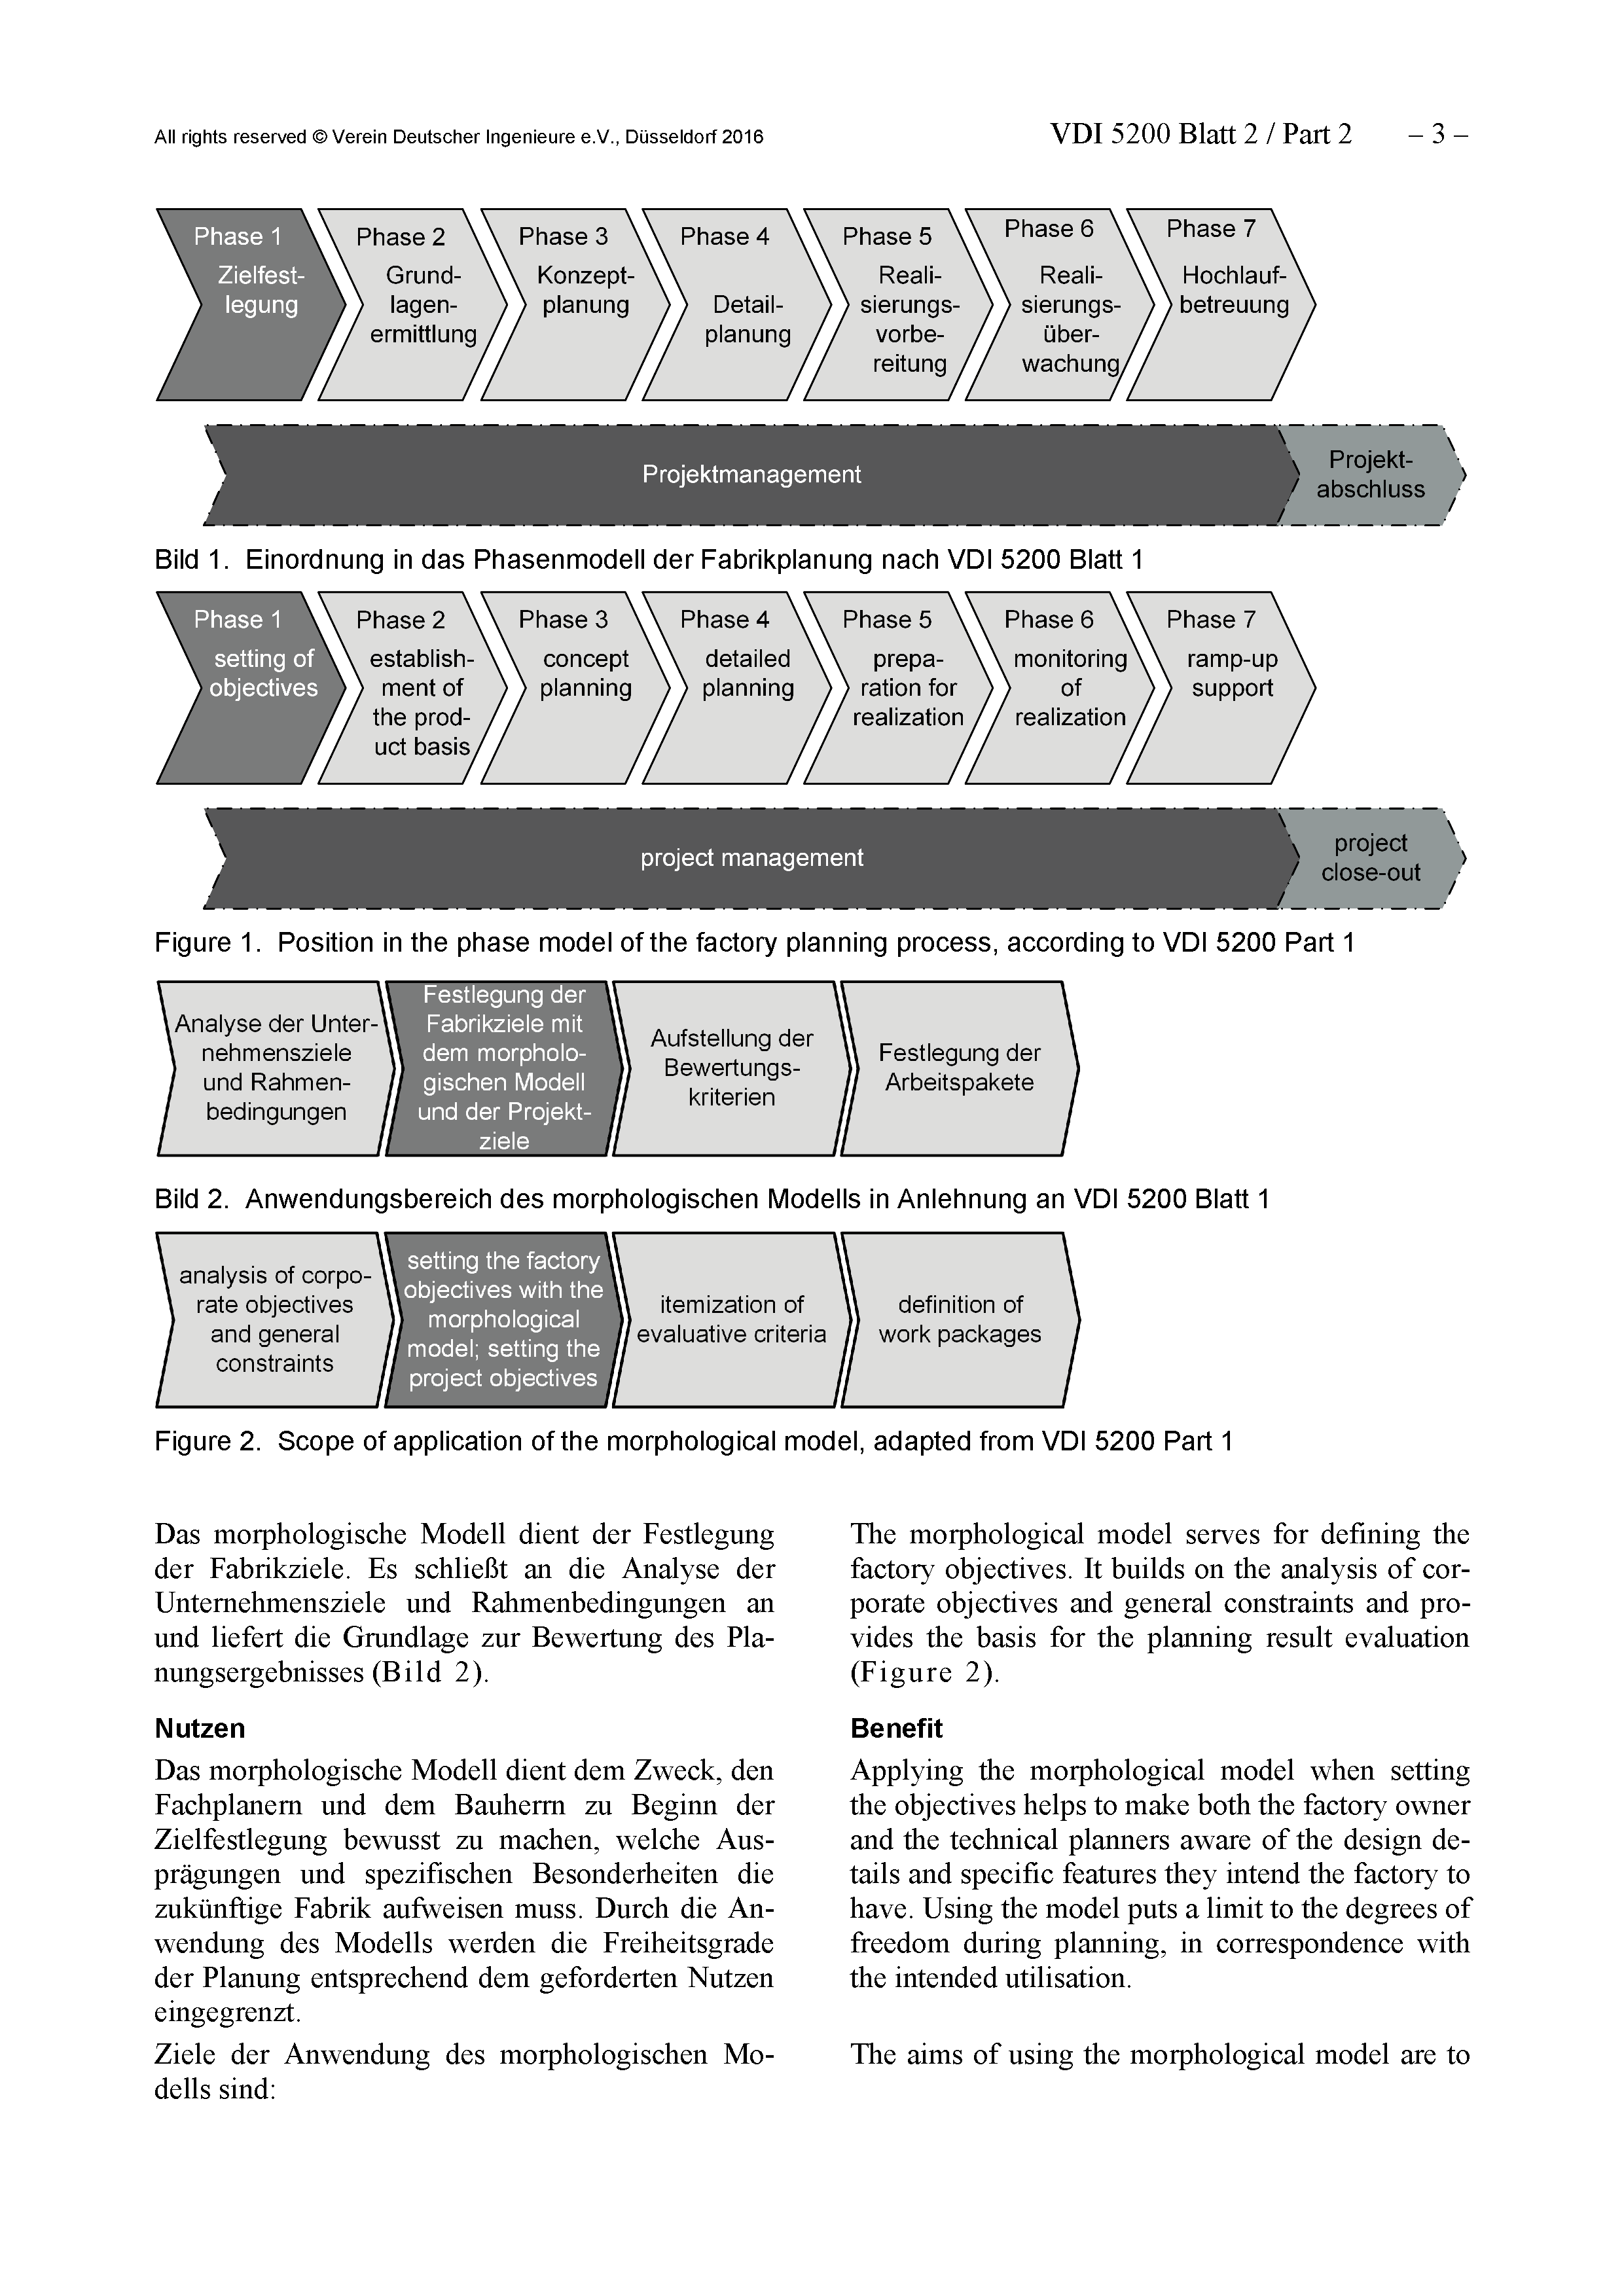
\includegraphics[trim={30pt 655pt 30pt 40pt},clip,width=\linewidth]{vdi5200_phasenmodell}
    \caption{Phasenmodell der Fabrikplanung nach VDI~5200 Blatt~1, Bild~1
        (Quelle: \cite{vdi5200}).}
    \label{fig:vdi5200_phasen}
\end{figure}

Das Phasenmodell ist dabei grundsätzlich sequenziell ausgerichtet, wobei spätere Phasen
auf den Ergebnissen früherer aufbauen. Klassischerweise werden die einzelnen Phasen
jedoch mit weitgehend eigenständigen, kaum miteinander verknüpften Modellen und
Werkzeugen bearbeitet.
Um diese Grenzen zwischen den Phasen zu überwinden, setzt die Digitale Fabrik auf ein
durchgängiges Datenmanagement, das alle Planungsphasen miteinander vernetzt.

\begin{figure}[H]
    \centering
    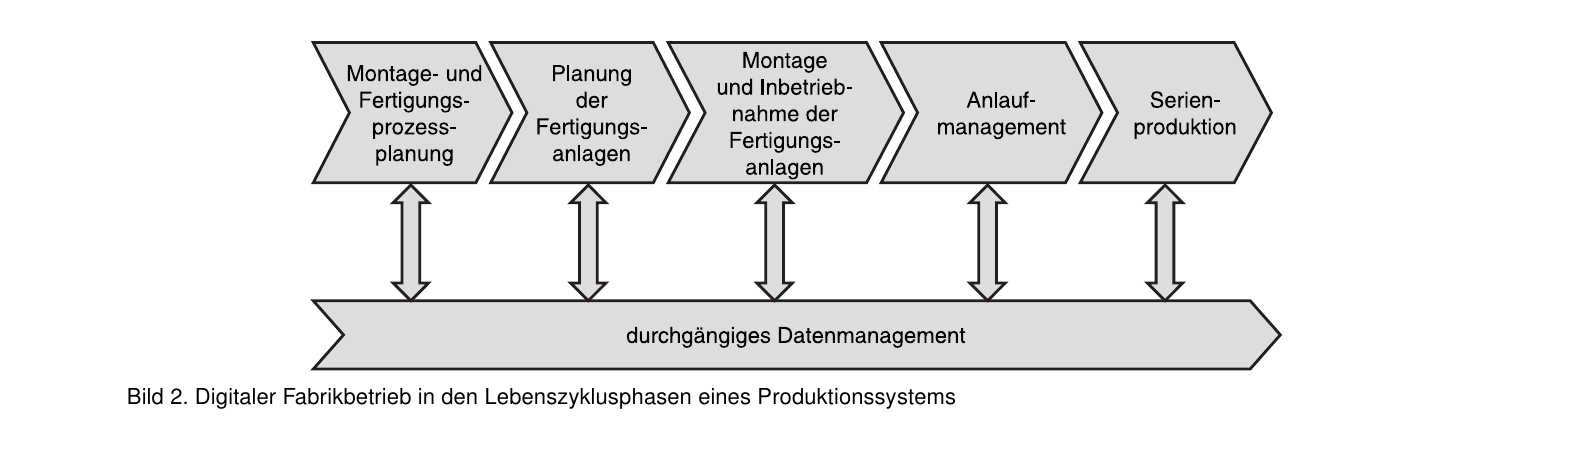
\includegraphics[width=\linewidth]{vdi4499_phasenmodell}
    \caption{Digitaler Fabrikbetrieb in den Lebenszyklusphasen eines Produktionssystems
        (Quelle: VDI~4499 Blatt~2 \cite{vdi4499b2}, Bild~2).}
    \label{fig:vdi4499_phasen}
\end{figure}

Das gezeigte Bild verdeutlicht, wie VDI~4499 Blatt~2 dieses Konzept in den
Lebenszyklusphasen eines Produktionssystems konkretisiert \cite{vdi4499b2}.
VDI~4499 Blatt~1 definiert die Digitale Fabrik als vernetztes System digitaler Modelle,
Methoden und Werkzeuge zur ganzheitlichen Planung und Steuerung von Fabrikprozessen
\cite{vdi4499} und schafft damit eine gemeinsame Datenbasis über alle Phasengrenzen hinweg.

\subsection{Virtuelle Inbetriebnahme nach VDI/VDE~3693}
\label{subsec:defizite}
Die \emph{Virtuelle Inbetriebnahme} (VIBN) setzt bereits in den Planungs- und
Realisierungsphasen an und ermöglicht es, Steuerungsprogramme und Produktionsabläufe
an einem digitalen Anlagenmodell zu erproben und zu optimieren, noch bevor die reale
Anlage fertiggestellt und die eigentliche Inbetriebnahme durchgeführt wird.
Die Richtlinie VDI/VDE~3693 Blatt~1 definiert VIBN als methodisches Vorgehen zur
frühzeitigen Absicherung der Steuerungssoftware vor der realen Inbetriebnahme einer
Anlage \cite{vdi3693} und unterscheidet dabei verschiedene Modellarten
(\emph{Software-in-the-Loop}, \emph{Hardware-in-the-Loop}).
Technische Grundlage bilden dabei cyber-physische Produktionssysteme (CPPS), die durch
bidirektionale Echtzeit-Kopplung zwischen physischer Anlage und digitalem Abbild die
Voraussetzung für Digitale Zwillinge schaffen \cite{monostori2014}.
Lechler et al.\ belegen empirisch, dass VIBN die Qualität und Effizienz im Engineering
steigert, Anlaufzeiten durch frühzeitige Fehlererkennung verkürzt und eine sicherere
Inbetriebnahme ermöglicht, indem erkannte Fehler bereits vor der realen Inbetriebnahme
behoben werden \cite{lechler2019}.

\subsection{Klassifikation Digitaler Zwillinge}
Um Digitale Zwillinge im Kontext dieser Arbeit präzise einordnen zu können, wird die
in der Literatur am weitesten verbreitete Klassifikation nach Kritzinger et al.
herangezogen.
Sie unterscheidet anhand des Datenflusses zwischen physischem Objekt und digitalem Abbild
drei Reifegrade \cite{kritzinger2018}.
\begin{itemize}
    \item \textbf{Digitales Modell:} Keine automatisierte Datenkopplung. Jegliche
        Aktualisierung zwischen physischem und digitalem Objekt erfolgt manuell.
    \item \textbf{Digitaler Schatten:} Ein automatisierter, unidirektionaler Datenfluss
        vom physischen zum digitalen Objekt. Das digitale Objekt spiegelt den Zustand
        des physischen wider, wirkt aber nicht auf dieses zurück.
    \item \textbf{Digitaler Zwilling:} Ein vollständig integrierter, in beide
        Richtungen automatisierter Datenfluss zwischen dem physischen und dem digitalen
        Objekt \cite{kritzinger2018}. Veränderungen am physischen Objekt führen
        unmittelbar zu Anpassungen des digitalen Abbildes und umgekehrt.
\end{itemize}
Diese Klassifikation bildet den Bewertungsmaßstab für den in den nachfolgenden Kapiteln
beschriebenen Umsetzungsgrad.

\iffalse
\subsubsection{Definition nach Stark und Damerau}
Stark und Damerau halten in der CIRP Encyclopedia of Production Engineering fest,
dass trotz intensiver Forschung bis heute keine einheitlich akzeptierte
wissenschaftliche Definition des Begriffs Digitaler Zwilling existiert.
Ihre Arbeit dokumentiert allein 19 verschiedene Definitionen aus der Literatur
\cite{stark2019}.
Den Ursprung des Konzepts führen sie auf Grieves zurück, der es 2002 an der University
of Michigan als \enquote{Mirrored Spaces Model} eingeführt hat.
Ihre eigene Definition lautet: Ein Digitaler Zwilling ist \enquote{ein digitales Abbild
eines aktiven, einzigartigen Produkts oder Produktionssystems, das durch ausgewählte
Eigenschaften, Bedingungen und Verhaltensweisen mittels Modellen, Informationen und
Daten charakterisiert wird} \cite{stark2019}.

Um zu verstehen, was das konkret bedeutet, unterscheiden Stark und Damerau drei
Bestandteile, die erst zusammen einen echten Digitalen Zwilling ergeben:

\textbf{(1) Digital Master:} Der \emph{Digital Master} ist das in der Entwicklungsphase
erstellte virtuelle Modell einer Anlage, das Geometrie, Kinematik und
Materialeigenschaften beschreibt.
Für den Maze Runner ist dies das aus CAD-Daten exportierte 3D-Modell in Isaac Sim,
das alle Bauteile originalgetreu abbildet.
Für den Dobot Magician ist es die kinematische Beschreibung des Roboterarms mit seinen
Gelenken, Drehachsen und Gelenklimits.

\textbf{(2) Digital Shadow:} Der \emph{Digital Shadow} sind die Echtzeitdaten, die die
physische Anlage laufend erzeugt: Sensorwerte, Schaltstellungen und Positionen.
Die Steuerungseinheit der physischen Anlage übermittelt diese Daten kontinuierlich an
das digitale Modell, sodass der aktuelle Betriebszustand stets im digitalen Abbild
sichtbar ist.

\textbf{(3) Verknüpfung:} Erst die Verbindung zwischen Konstruktionsmodell und
Livedaten erzeugt den eigentlichen Digitalen Zwilling.
Eine Middleware-Schicht liest die Betriebsdaten der physischen Anlage aus und setzt sie
in Bewegungsänderungen des digitalen Modells um, sodass beide Instanzen synchron laufen.

Besonders betonen Stark und Damerau den Aspekt der \emph{Einzigartigkeit}: Ein
Digitaler Zwilling bildet stets eine bestimmte physische Instanz ab, nicht ein
generisches Produktionslinienmodell.
\fi

\subsection{Digitale Zwillinge im Fertigungskontext}
Die Klassifikation nach Kritzinger et al.\ beschreibt, in welchem Maß der Datenfluss
zwischen physischem Objekt und digitalem Abbild automatisiert ist.
Sie beantwortet damit die Frage nach dem Kopplungsgrad, beschreibt aber nicht, welche
physischen Elemente beobachtet werden können und wie das Gesamtsystem dabei strukturiert ist.
Die Normenreihe ISO~23247 schließt diese Lücke und beschreibt das Digital-Twin-Framework
für die Fertigung als schichtbasiertes IoT-Rahmenwerk, das Abbildung~\ref{fig:dt_manufacturing}
veranschaulicht.

\begin{figure}[H]
    \centering
    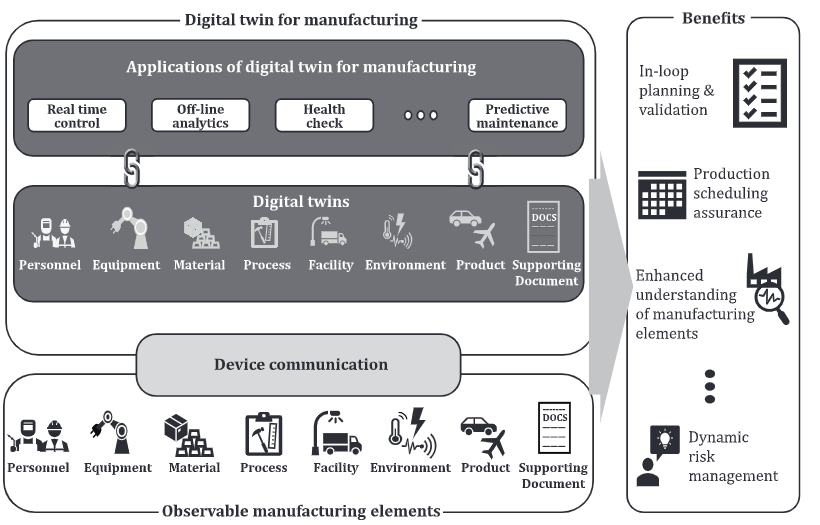
\includegraphics[width=\linewidth]{DT for manufacturing}
    \caption{IoT-Rahmenwerk für Digitale Zwillinge in der Fertigung mit Anwendungsschicht,
        Digitalem Zwilling, Gerätekommunikation und beobachtbaren Fertigungselementen
        (Quelle: ISO/FDIS~23247-1 \cite{iso23247}, Figure~2).}
    \label{fig:dt_manufacturing}
\end{figure}

Das Framework gliedert sich in drei Schichten.
Die Anwendungsschicht umfasst Funktionen wie Echtzeitsteuerung, Offline-Analytik und
vorausschauende Wartung, die auf den Digitalen Zwilling zugreifen.
Der Digitale Zwilling bildet die mittlere Schicht und repräsentiert je nach Anwendungsfall
eines oder mehrere der acht beobachtbaren Fertigungselemente.
Diese umfassen Personal, Betriebsmittel, Material, Fertigungsprozesse,
Fertigungsinfrastruktur, Umgebung, Produkt und Begleitdokumente \cite{iso23247}.
Die Gerätekommunikation verbindet den Digitalen Zwilling bidirektional mit den physischen
Fertigungselementen und übernimmt den Datentransport zwischen realer Anlage und
digitalem Abbild.
Rechts der Abbildung sind zudem Nutzenpotenziale aufgeführt, die Digitale Zwillinge
in der Fertigung erschließen, darunter Echtzeitregelung, Produktionsplanung und
vorausschauende Risikobewertung \cite{iso23247}.
Die Darstellung vermittelt damit einen anschaulichen ersten Überblick über das
Zusammenspiel von digitalem Abbild, Gerätekopplung und Anwendungsnutzen.

\subsection{Referenzarchitekturmodell RAMI~4.0}
An Planung, Umsetzung und Betrieb vernetzter Industrie-4.0-Anlagen sind Fachleute
aus verschiedenen Disziplinen beteiligt. Jede Disziplin beschreibt Komponenten in
eigenen Begriffen, sodass Zuständigkeiten über Systemgrenzen hinweg schwer
abzustimmen und Probleme an Schnittstellen schwer einzugrenzen sind.
Für die Einordnung nach Betriebsebene diente traditionell die Automatisierungspyramide,
die Feldgeräte, Steuerungen und IT-Systeme in eine vertikale Hierarchie gliedert.
Sie erfasst jedoch weder den Produktlebenszyklus noch die Architekturschichten, die
für eine vollständige Beschreibung vernetzter Industrie-4.0-Komponenten notwendig sind.
Das Referenzarchitekturmodell RAMI~4.0 (DIN~SPEC~91345) schließt diese Lücke und
erweitert die Automatisierungspyramide um die Achsen Lebenszyklus und Wertschöpfung
sowie sechs Architekturschichten. Es stellt damit den dreidimensionalen Rahmen bereit,
in dem sich Maschinen, Anlagen, Softwarekomponenten und Digitale Zwillinge einheitlich
beschreiben und zueinander in Beziehung setzen lassen \cite{dinspec91345}.
Das Modell richtet sich an alle Akteursgruppen, die an Industrie-4.0-Systemen
mitwirken.

\begin{itemize}
    \item Maschinenbauer und Anlagenbauer (mechanische Konstruktion, Steuerungstechnik)
    \item Elektro- und Automatisierungsingenieure (SPS, Feldbusse, Sensorik)
    \item IT-Architekten und Softwareentwickler (Cloud, MES, ERP-Anbindung)
    \item Inbetriebnehmer vor Ort
    \item Betreiber und Produktionsplaner
    \item Systemintegratoren
    \item Normungsgremien und Zertifizierungsstellen
\end{itemize}

In Abbildung~\ref{fig:rami40} ist das Modell als dreidimensionale Struktur dargestellt.

\begin{figure}[H]
    \centering
    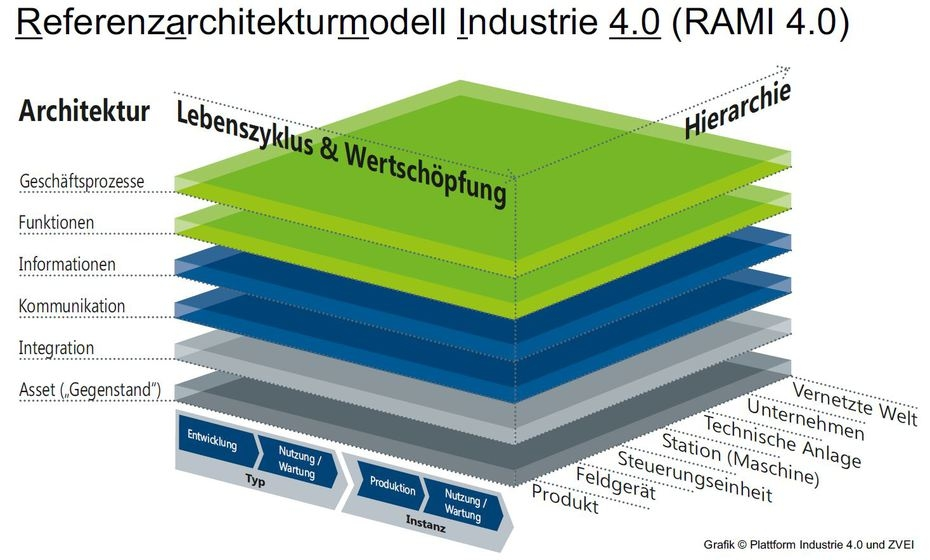
\includegraphics[width=\linewidth]{rami.jpg}
    \caption{RAMI~4.0: Referenzarchitekturmodell Industrie~4.0 als dreidimensionales
        Schichtenmodell mit den Achsen \enquote{Life Cycle \& Value Stream},
        \enquote{Hierarchy Levels} und \enquote{Layers}
        (Quelle: DIN~SPEC~91345 \cite{dinspec91345}).}
    \label{fig:rami40}
\end{figure}

Grundlegende Einheit des Modells ist das \textbf{Asset}, worunter jedes physische
oder virtuelle Objekt mit definierten Eigenschaften und Wert verstanden wird, vom
einzelnen Sensor über eine Steuerungseinheit bis zur gesamten Anlage.
Für jedes Asset kann eine Verwaltungsschale (Asset Administration Shell) angelegt
werden, die seine Eigenschaften und Fähigkeiten maschinenlesbar digital repräsentiert.

Die \textbf{Hierarchieachse} übernimmt die Struktur der Automatisierungspyramide mit
den Ebenen Feldgerät, Steuerungseinheit, Arbeitsstation und Arbeitszelle und ergänzt
sie um Betrieb sowie Vernetzte Welt, welche übergeordnete Cloud- und IoT-Dienste
einschließt. Jedes Asset lässt sich einer oder mehreren dieser Ebenen zuordnen.

In vertikaler Richtung gliedern sechs \textbf{Architekturschichten} jede Hierarchieebene
und beschreiben, welche Fähigkeiten ein Asset dort bereitstellt. Sie umfassen die Schichten Asset (die physische Komponente selbst),
Integration, Kommunikation, Information, Funktionen und Geschäftsprozesse.
Kommunikationsstandards wie OPC~UA sind der Kommunikationsschicht zuzuordnen,
Datenformate wie OpenUSD der Informationsschicht.

Die dritte Achse erfasst den \textbf{Lebenszyklus} eines Assets von der Entwicklung
über den Betrieb bis zur Außerbetriebnahme und unterscheidet dabei zwischen Typ, dem
allgemeinen Modell einer Komponente, und Instanz, dem konkreten Exemplar im Einsatz.
Digitale Zwillinge bilden stets Instanzen ab, da sie den aktuellen Zustand einer
bestimmten physischen Anlage repräsentieren.

Damit steht Maschinenbauern, Elektroingenieuren, IT-Architekten und Inbetriebnehmern
eine gemeinsame Beschreibungssprache zur Verfügung. Systeme lassen sich
schichtenweise analysieren, Schnittstellen eindeutig verorten und Probleme an
Systemgrenzen gezielt eingrenzen, ohne das Gesamtsystem vollständig durchleuchten
zu müssen.

\subsection{Normativer Rahmen nach ISO~23247}

Im vorangehenden Unterkapitel wurde das Digital-Twin-Framework in seiner Grundstruktur
dargestellt.
Eine formale Beschreibung der einzelnen Entitäten und ihrer Schnittstellen fehlt darin.
Für Fertigungsumgebungen liegt mit ISO~23247 ein internationaler Standard vor, der
diesen Rahmen beschreibt.
Sie ist in vier Teile gegliedert. Teil~1 beschreibt allgemeine Grundsätze und
Anforderungen, Teil~2 die Referenzarchitektur mit funktionalen Sichten, Teil~3
die Informationsattribute der beobachtbaren Fertigungselemente und Teil~4 die
technischen Anforderungen an den Informationsaustausch \cite{iso23247}.

Das in Teil~2 spezifizierte \emph{Digital Twin Framework} unterscheidet dabei zwei
funktional verschiedene Einsatzkontexte.
Im Unternehmenskontext sind Aspekte wie die Integration übergeordneter Systeme
(ERP, MES), rollenbasierte Zugangskontrolle sowie die Vernetzung mehrerer Zwillinge
untereinander über die Cross-System Entity bedeutsam.
Für einen Digitalen Zwilling als eigenständige Instanz, die eine einzelne physische
Anlage konsistent abbildet, stehen hingegen die Core Entity als Träger der digitalen
Repräsentation und die \emph{Data Collection and Device Control Entity} (DCDCE) als Kommunikationsschicht zur realen Anlage im Vordergrund.
Abbildung~\ref{fig:iso23247} zeigt das funktionale Referenzmodell des Frameworks mit
der hierarchischen Anordnung seiner vier Entitäten.

\begin{figure}[H]
    \centering
    \includegraphics[width=0.85\linewidth]{{Functional view of the Digital Twin reference model for manufacturing}}
    \caption{Funktionale Referenzarchitektur des Digital Twin Frameworks für die Fertigung
        mit User Entity, Core Entity, Data Collection and Device Control Entity
        und Cross-System Entity sowie den beobachtbaren Fertigungselementen außerhalb
        der Frameworkgrenze
        (Quelle: \cite{iso23247}).}
    \label{fig:iso23247}
\end{figure}

Ein Digitaler Zwilling, der eine einzelne Fertigungsanlage mit zugehöriger
Nutzerschnittstelle abbildet, ohne in Unternehmenssysteme eingebettet zu sein oder
auf weitere Zwillinge zuzugreifen, erfordert primär die direkte Kopplung zwischen
physischer und digitaler Welt.
Die \textbf{DCDCE} ist dabei die funktional zentrale Entität. Sie erfasst kontinuierlich
die Zustandsdaten der physischen Anlage, leitet sie an die Core Entity weiter und
übersetzt in Gegenrichtung Steuerbefehle in Signale für die physische Anlage.
Den Kommunikationsteil dieser Entität bildet eine Middleware-Schicht, die den
Datentransport zur physischen Anlage übernimmt. Protokolle wie OPC~UA oder ROS~2 werden
in dieser Rolle eingesetzt. Die DCDCE reicht jedoch über den reinen Datentransport
hinaus und umfasst auch die Steuerungslogik für Gerätebefehle sowie die
Synchronisationsschnittstelle zur Core Entity.

Die \textbf{Core Entity} strukturiert ihre Funktionen über mehrere Functional Interfaces.
Für einen eigenständigen Digitalen Zwilling sind die Schnittstellen für digitale
Modellbildung (\emph{Digital Modeling FI}), Datensynchronisation (\emph{Synchronization FI})
und physikalische Simulation (\emph{Simulation FI}) zentral.
Die \emph{Reporting FI} ermöglicht die strukturierte Ausgabe von Zustandsdaten.
Die \emph{Peer Interface FI}, die der direkten Verbindung mit weiteren Digitalen Zwillingen
dient, ist für einen Zwilling ohne Vernetzungsanforderung nicht relevant.

In ISO~23247 werden acht Typen beobachtbarer Fertigungselemente unterschieden,
sogenannte \emph{Observable Manufacturing Elements} (OME) \cite{iso23247}.
Fertigungsanlagen und Betriebsmittel werden dem Typ \emph{Equipment} zugeordnet,
die durch sie ausgeführten Operationen dem Typ \emph{Process}.
Das in der Anlage verarbeitete oder beförderte Werkstück ordnet die Norm dem Typ
\emph{Product} zu und trennt es damit konzeptuell von der Fertigungsanlage selbst.

\subsection{NVIDIA Omniverse-Ökosystem}
\label{subsec:omniverse}
NVIDIA Omniverse ist eine GPU-beschleunigte Kollaborationsplattform, die
Engineering-Werkzeuge verschiedener Hersteller über Konnektoren in OpenUSD-Szenen
zusammenführt, Änderungen über den Nucleus-Server im 24/7-Dauerbetrieb zwischen
allen Clients synchronisiert und Anlage sowie Produkt parallel in derselben Szene
simuliert \cite{nvidia_omniverse}.
Als Simulationsanwendung des Ökosystems verbindet \emph{Isaac Sim} physikalisch
korrekte Starrkörperdynamik mit fotorealistischem RTX-Rendering und wird in dieser
Arbeit für die Entwicklung der Digitalen Zwillinge eingesetzt \cite{nvidia_isaacsim}.
Auch in der Automobilindustrie wird Omniverse für die virtuelle Fabrikplanung
eingesetzt, um Planungsdaten verschiedener Werkzeuge ohne Kompatibilitätshürden in
einer gemeinsamen Simulationsumgebung zusammenzuführen \cite{bmw_nvidia_2021}.
Wie eine solche Simulation in Isaac Sim aussieht, zeigt Abbildung~\ref{fig:isaac_bmw}.

\begin{figure}[H]
    \centering
    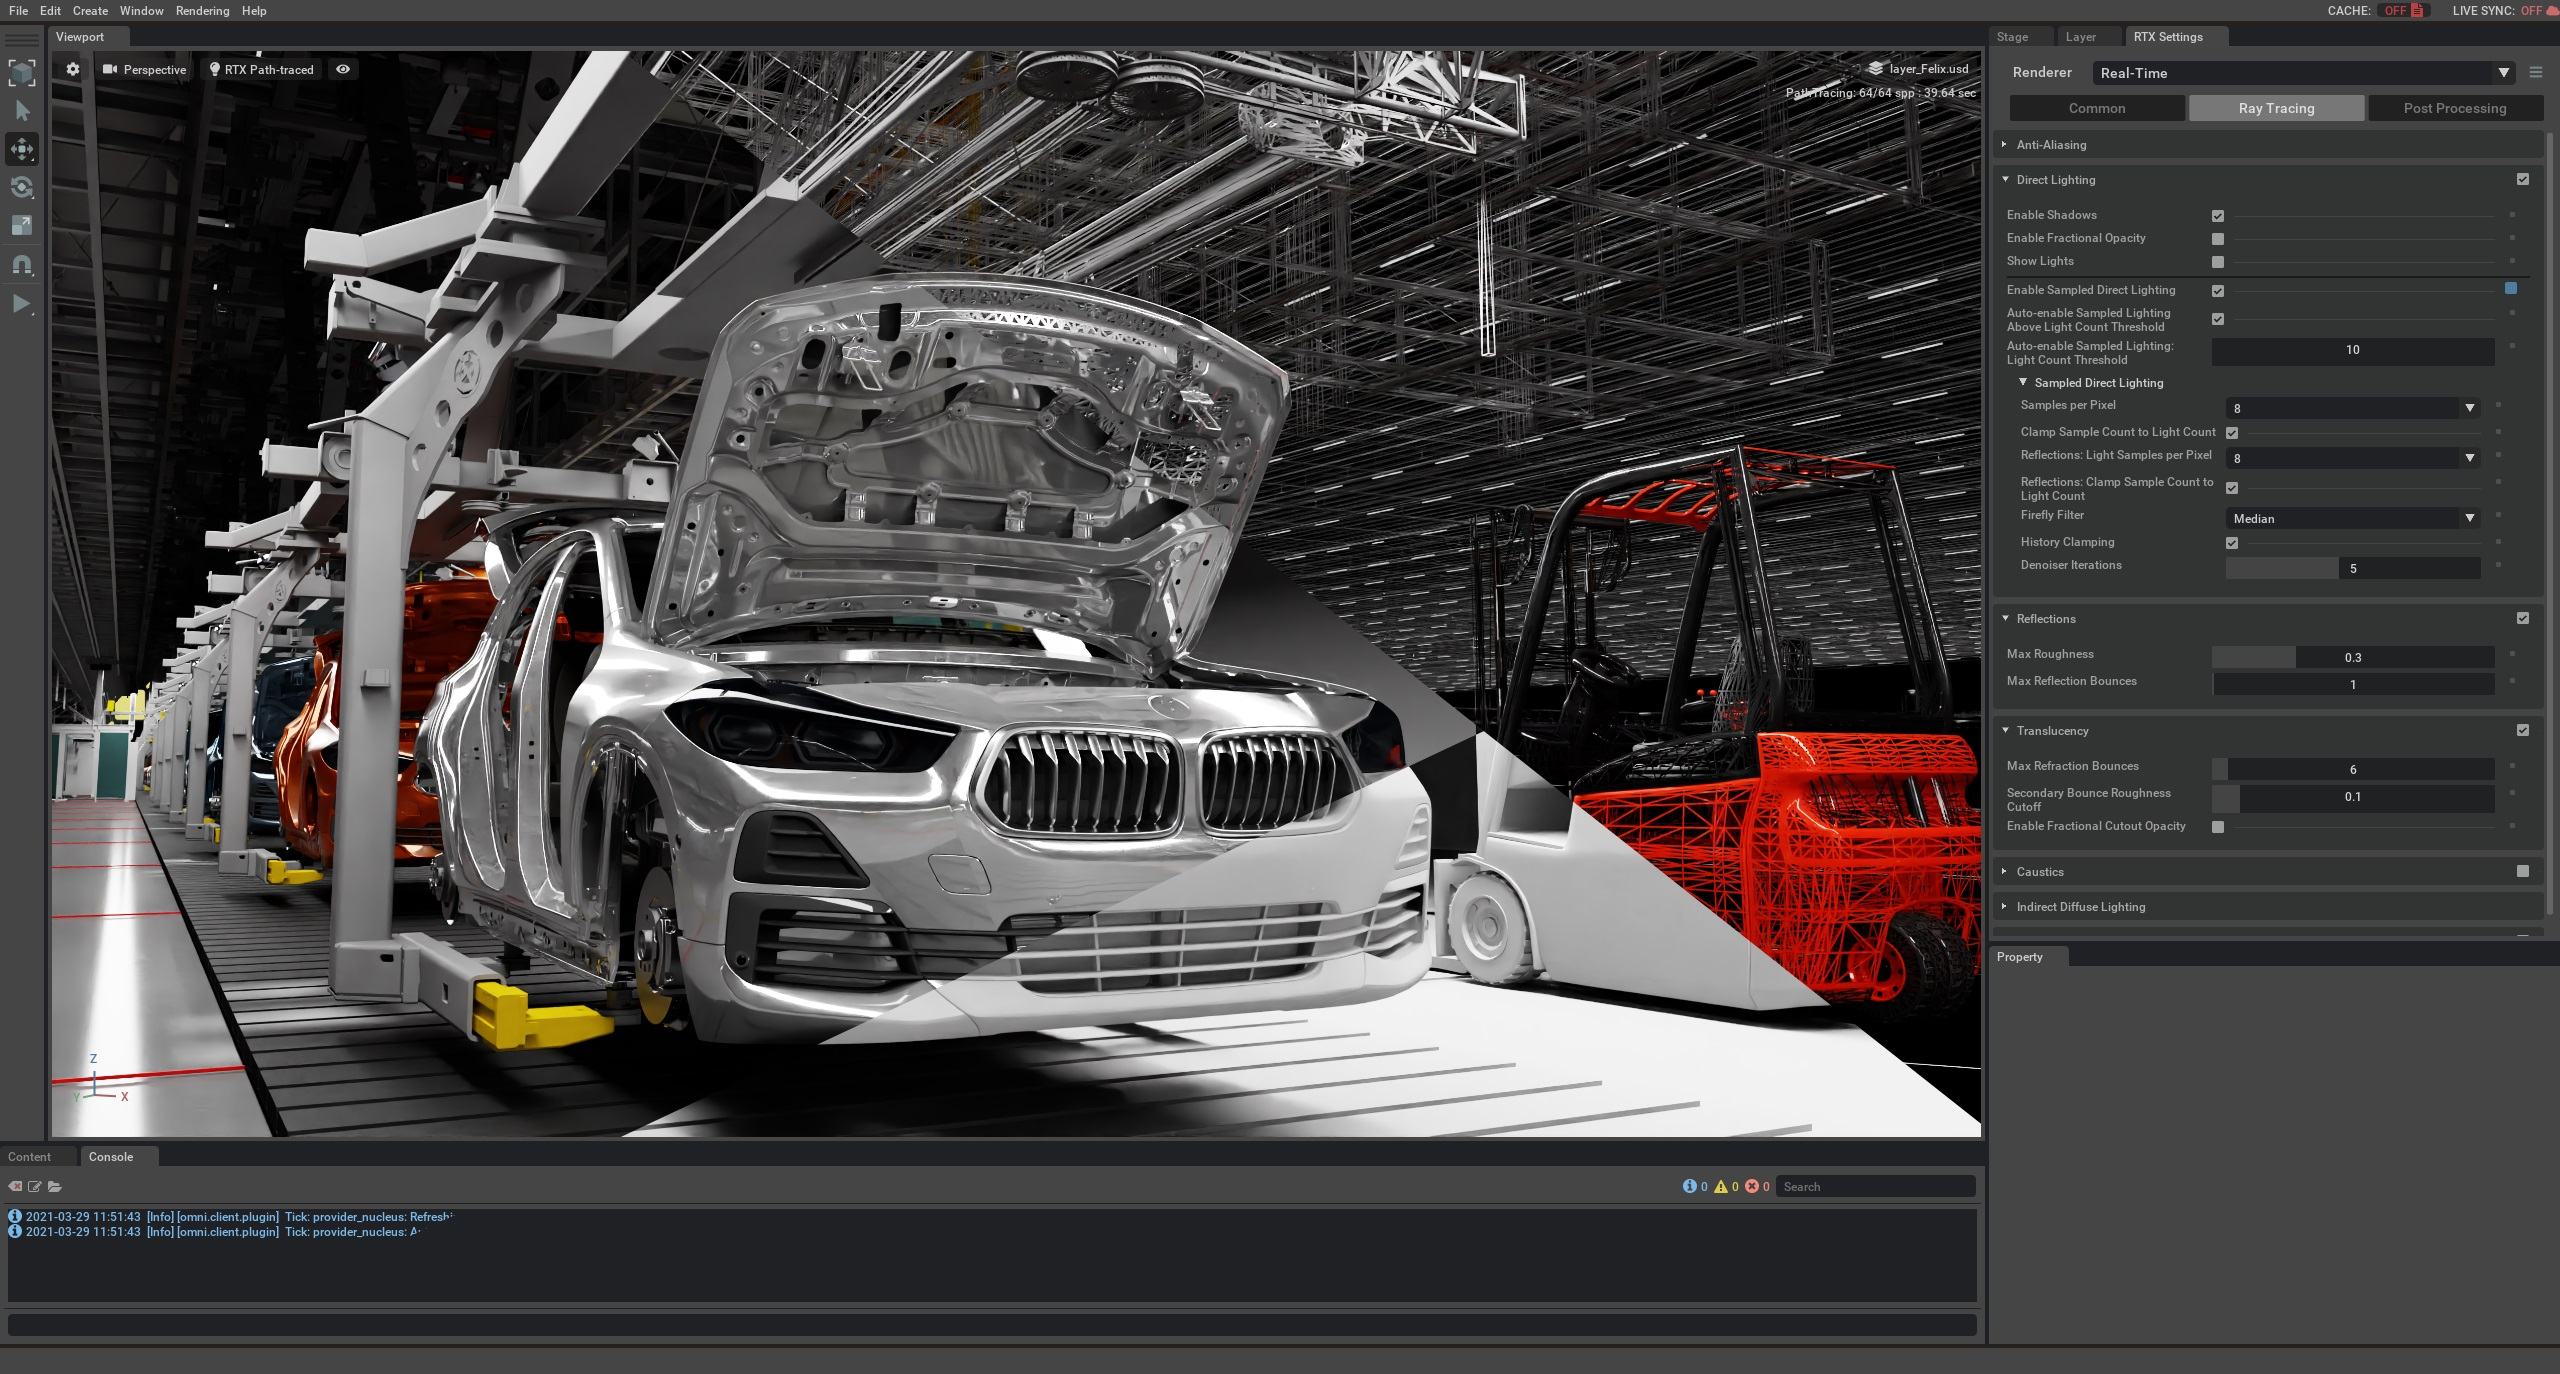
\includegraphics[width=\linewidth]{BMW_Isaac Sim.jpg}
    \caption{NVIDIA Isaac Sim Viewport mit aktiviertem RTX Path Tracing. Simultane
        Darstellung unterschiedlicher Verarbeitungszustände in einer USD-Szene
        \cite{bmw_nvidia_2021}}
    \label{fig:isaac_bmw}
\end{figure}

Im Viewport sind gleichzeitig unterschiedliche Darstellungszustände einer USD-Szene
sichtbar.
Die Karosserie im Vordergrund ist vollständig mit RTX Path Tracing berechnet.
Reflexionen auf der Metalloberfläche und der Schattenwurf entstehen durch physikalisch
basierte Lichtpfadsimulation.
Der rechte Szenenbereich, bestehend aus Gabelstapler, Hallendecke und angrenzenden
Strukturen, wird im Wireframe-Modus dargestellt und repräsentiert approximierte
Kollisionsgeometrien.
Gabelstapler und Teile der Frontschürze sind mit einem weißen Standardmaterial
versehen, das Omniverse automatisch zuweist, wenn keine Materialdefinition im
Datensatz vorhanden ist.

\emph{Omniverse Kit} als Kern der Plattform ist ein erweiterbares
Anwendungsframework mit drei Eigenschaften, die es von klassischen
Fabrikplanungswerkzeugen unterscheiden.

\begin{itemize}
    \item \textbf{Konnektoreninfrastruktur:} Omniverse bindet bestehende
        Engineering-Werkzeuge über sogenannte \emph{Connectors} an, die
        herstellerspezifische Daten in OpenUSD übersetzen und einen bidirektionalen
        Datenaustausch herstellen. Dies umfasst Anbindungen an CAD-, BIM- und
        PLM-Systeme wie Autodesk Revit, Siemens NX und PTC Creo
        \cite{nvidia_omniverse_connectors}. Bestandsmodelle lassen sich so ohne
        manuellen Konvertierungsaufwand in einer gemeinsamen Szene zusammenführen.
    \item \textbf{Nucleus als zentrale Kollaborationsschicht:} Das technische Rückgrat
        bildet der \emph{Omniverse Nucleus} (\emph{database and collaboration engine}),
        an dem mehrere Clients gleichzeitig live verbunden sind. Änderungen an den
        Modellen werden in Echtzeit zwischen allen Clients synchronisiert, wobei die
        Plattform als Enterprise-Variante für einen hochverfügbaren 24/7-Dauerbetrieb
        in produktionsnahen Szenarien ausgelegt ist \cite{nvidia_nucleus_arch}.
    \item \textbf{Parallele Simulation von Anlage und Produkt:} Basierend auf dem
        NVIDIA DSX Blueprint für AI-Factory-Digitale-Zwillinge werden Geometrie-,
        thermische und elektrische Simulationsdaten verschiedener Disziplinen über
        USD-Layer verknüpft. Sowohl die Anlage als auch das prozessierte Produkt liegen
        in derselben Szene als parallel simulierbare Entitäten vor
        \cite{nvidia_omniverse}.
\end{itemize}

Isaac Sim wird mit einem vorinstallierten Extension-Katalog ausgeliefert, der
allgemeine Werkzeuge innerhalb der Simulationsumgebung bereitstellt, wie eine
VR-Experience oder den Script Editor, über den Python-Code direkt in der laufenden
Szene ausgeführt werden kann.

Das physikalische Fundament der Simulation bildet die Physik-Engine \emph{PhysX},
die Starrkörperdynamik, Gelenkkräfte und Kollisionserkennung GPU-parallel berechnet
\cite{nvidia_physx}.
PhysX ist zudem in verbreiteten Simulationsumgebungen wie Visual Components oder
KUKA.Sim integriert.

Zum Omniverse-Ökosystem gehören weitere spezialisierte Anwendungen.
\textbf{Isaac Lab} erweitert Isaac Sim um ein Framework für Reinforcement Learning,
mit dem Roboter-Verhaltensweisen trainiert und per Sim-to-Real-Transfer auf reale
Hardware übertragen werden können, wie in Abbildung~\ref{fig:isaac_lab} gezeigt
\cite{nvidia_isaaclab}.
Als drittes Glied der Isaac-Familie zeichnet \textbf{Isaac TeleOp} menschliche
Bedienabläufe als Trainingsdaten auf, wobei verschiedene Eingabegeräte wie etwa
VR-Brillen verwendet werden, wie in Abbildung~\ref{fig:isaac_teleop} gezeigt
\cite{nvidia_isaacteleoperation}.
\textbf{Isaac GR00T} stellt ein Grundlagenmodell für humanoide Roboter bereit und
kann aus den von Isaac TeleOp aufgezeichneten Bewegungsabläufen humanoide Roboter
trainieren, wie in den Abbildungen~\ref{fig:isaac_lab} und~\ref{fig:isaac_teleop}
gezeigt \cite{nvidia_groot}.
\textbf{Isaac ROS} ist für Mobilitätsanwendungen bis hin zum autonomen Fahren
ausgelegt \cite{nvidia_isaacros}.
Um eine ausreichende Datensatzvielfalt für KI-Modellanwendungen sicherzustellen,
wurde \textbf{NVIDIA Cosmos} entwickelt, um aus bestehenden Simulationsszenen
Variationen in Beleuchtung, Textur und Materialeigenschaften zu erzeugen
\cite{nvidia_cosmos}.

\begin{figure}[H]
    \centering
    \begin{minipage}[t]{0.48\linewidth}
        \centering
        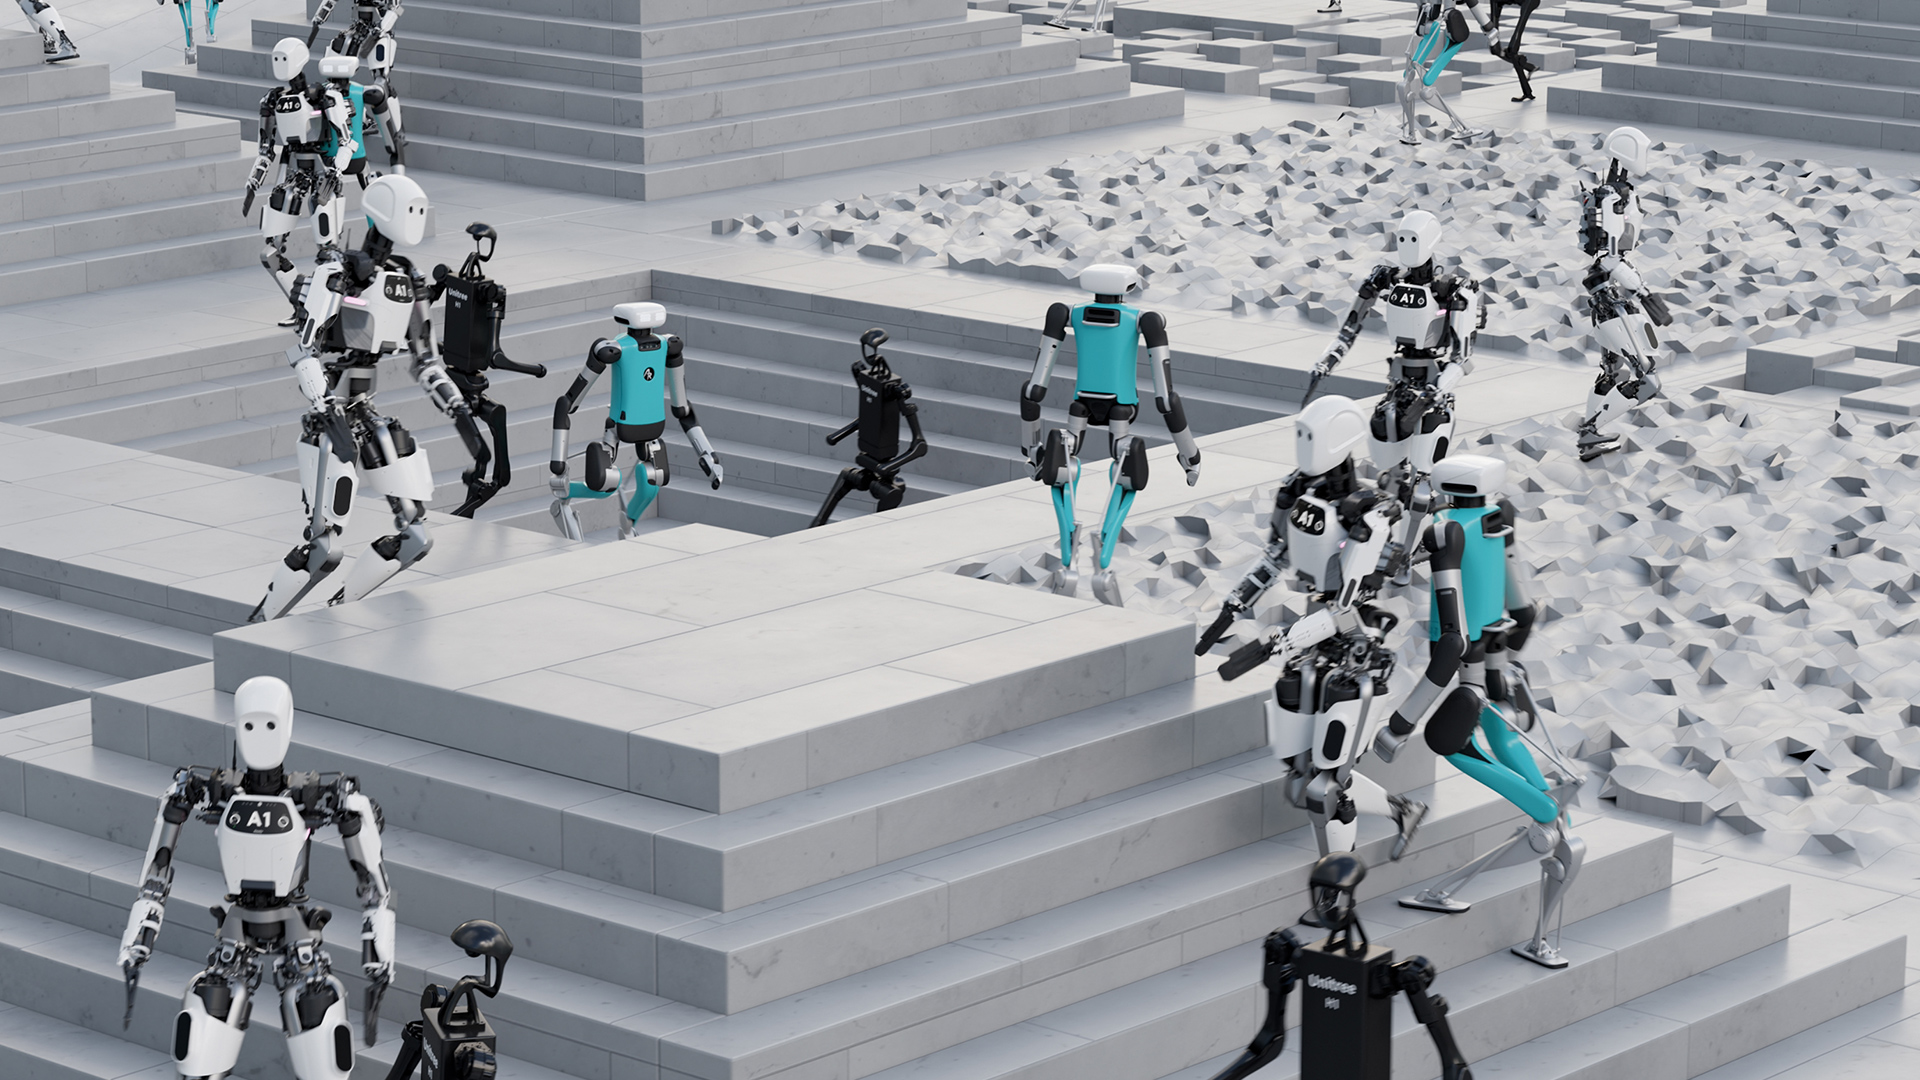
\includegraphics[width=\linewidth]{isaac lab.png}
        \caption{Paralleles Training von Robotern in NVIDIA Isaac Lab
            \cite{nvidia_isaaclab}}
        \label{fig:isaac_lab}
    \end{minipage}
    \hfill
    \begin{minipage}[t]{0.48\linewidth}
        \centering
        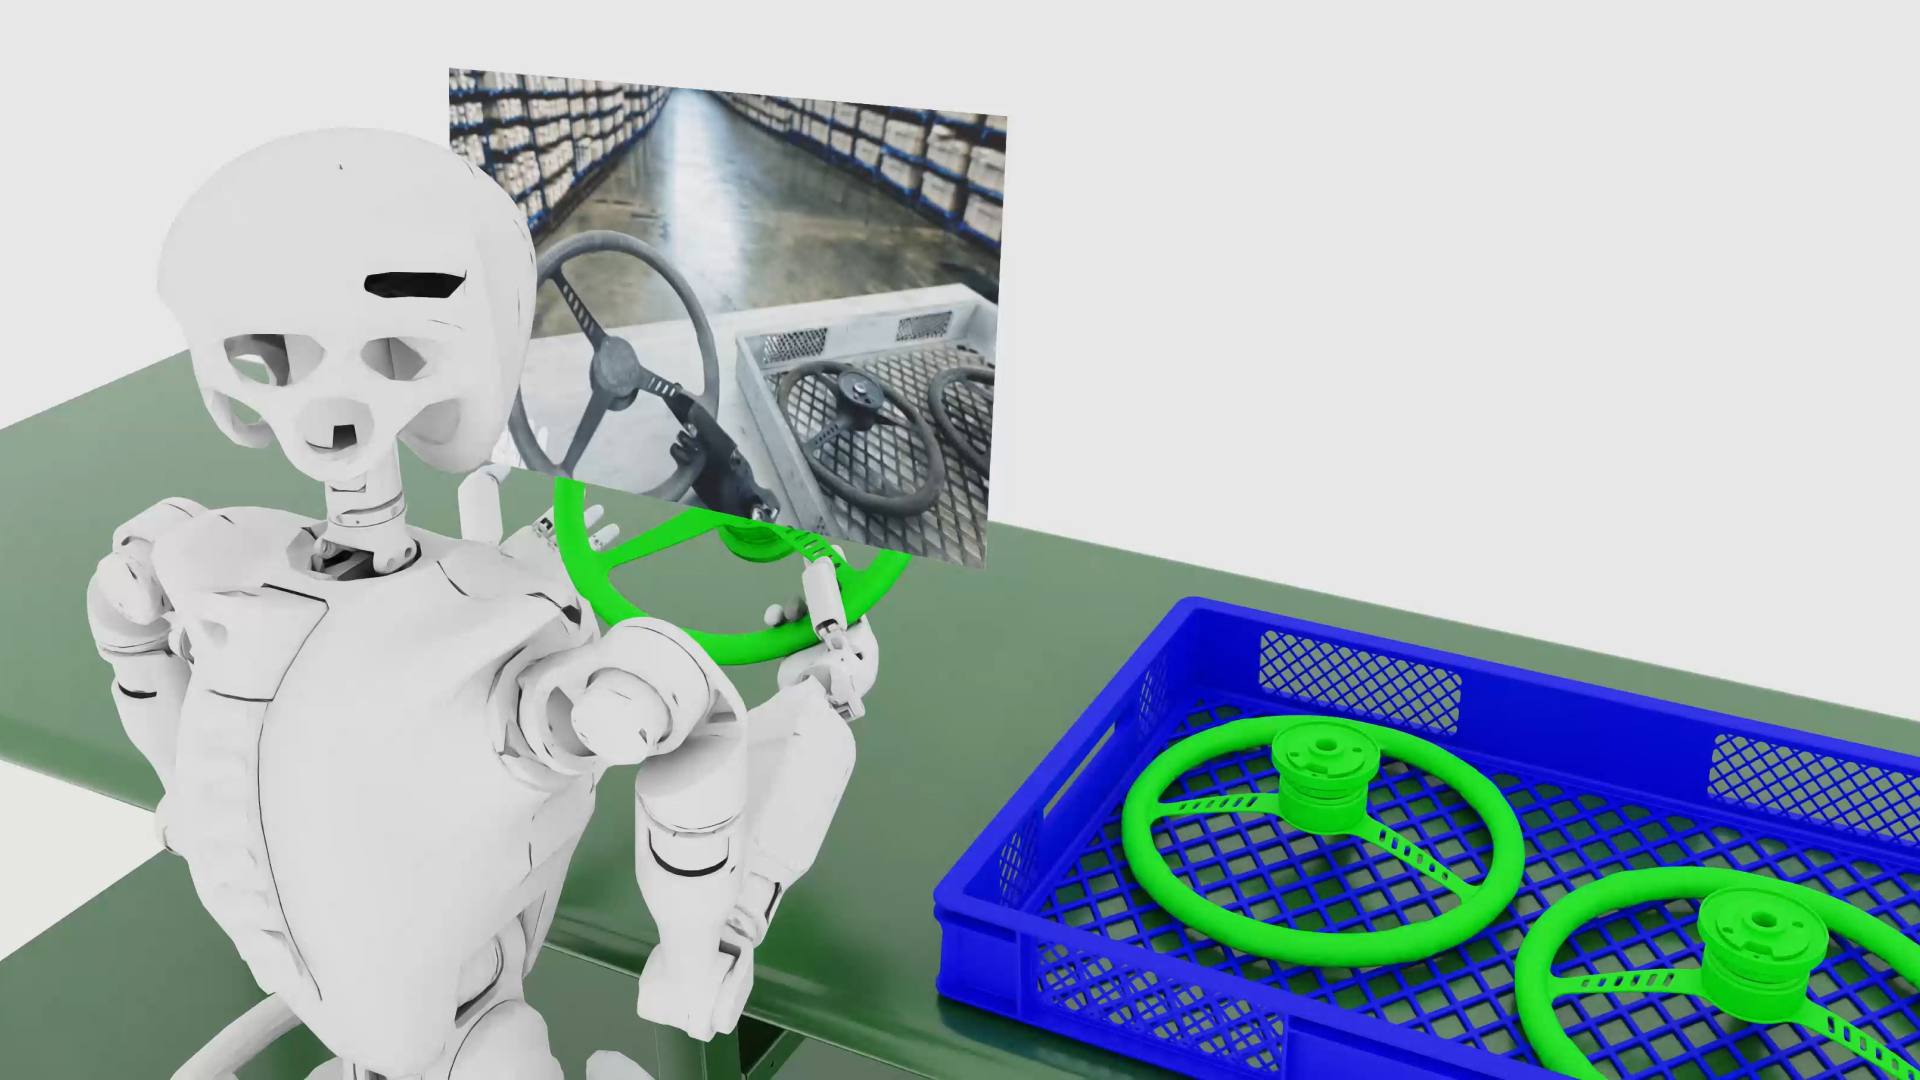
\includegraphics[width=\linewidth]{NVIDIA Cosmos.png}
        \caption{Erfassen und Übertragen menschlicher Bedienabläufe per VR-Brille
            mit Isaac TeleOp und Isaac GR00T
            \cite{nvidia_isaacteleoperation,nvidia_groot}}
        \label{fig:isaac_teleop}
    \end{minipage}
\end{figure}


\subsection{Datenformate OpenUSD und URDF}
\label{subsec:datenformate}
Das von Pixar Animation Studios entwickelte Format \emph{Universal Scene Description}
(OpenUSD) organisiert Szenendaten als hierarchischen Namensraum aus \emph{Prims}
(Primitives) \cite{pixar_openusd}.
NVIDIA Omniverse nutzt OpenUSD als natives Dateiformat, sodass CAD-Geometrien,
Simulationsparameter und Laufzeitdaten verschiedener Planungsphasen ohne
werkzeugspezifische Konvertierungen in einer gemeinsamen Szene zusammenwachsen
\cite{nvidia_omniverse}.
Dies schafft auf Datenformatsebene die Grundlage für das durchgängige Datenmodell,
das VDI~4499 als Ziel der Digitalen Fabrik beschreibt.

Für die roboterspezifische Strukturbeschreibung ergänzt das \emph{Unified Robot
Description Format} (URDF) das OpenUSD-Ökosystem \cite{ros_urdf}.
URDF formalisiert kinematische Glieder (\emph{links}), Gelenke (\emph{joints}) sowie
visuelle, kollisions- und trägheitsrelevante Geometrien in einer XML-Struktur und wird
in der Robotik als verbreitetes Standardbeschreibungsformat eingesetzt \cite{ros_urdf}.


\subsection{Middleware-Architekturen für die industrielle Kommunikation}

Middleware-Architekturen bilden die kommunikative Brücke zwischen der physischen Anlage
und der Omniverse-Extension, die den digitalen Zwilling in der Simulationsszene steuert.
Sie übernehmen den Transport von Sensordaten, Steuerungsbefehlen und Zustandsinformationen
in Echtzeit.
Die im Folgenden vorgestellten Protokolle OPC~UA, MQTT und ROS~2 sind industriell
etabliert, weit verbreitet und decken unterschiedliche Anforderungen an Semantik,
Bandbreite und Echtzeitfähigkeit ab.

\subsubsection{OPC UA (DIN EN IEC 62541)}
Im Client-Server-Modell stellt die Steuerungseinheit einer Anlage als OPC~UA-Server
Maschinensignale und Zustandsdaten strukturiert bereit.
Ein Client liest Sensorwerte aus und schreibt bei Bedarf Sollwerte zurück.
Integrierte Sicherheitsmechanismen und plattformunabhängige Implementierung haben
OPC~UA zum verbreiteten Standard für die vertikale Integration in
Industrie~4.0-Architekturen gemacht.
Das Protokoll \emph{Open Platform Communications Unified Architecture} (OPC~UA) ist in
der Normenreihe DIN~EN~IEC~62541 festgeschrieben \cite{iec62541}.

\subsubsection{MQTT v5.0}
Im Publish-Subscribe-Ansatz veröffentlichen Sender Nachrichten an einen Broker,
der sie an alle Abonnenten des jeweiligen Themas weiterleitet, was MQTT~5.0
besonders für ressourcenbeschränkte IoT-Knoten geeignet macht.
Das Protokoll \emph{Message Queuing Telemetry Transport} (MQTT) ist in Version~5.0
von OASIS standardisiert \cite{oasis_mqtt5}.

\subsubsection{ROS 2 und DDS}
ROS\,2 ist für die Ansteuerung kinematischer Ketten ausgelegt, da Gelenkwinkel von
Roboterarmen über standardisierte Nachrichtentypen in Echtzeit übertragen werden.
Konfigurierbare \emph{Quality-of-Service}-Profile erlauben es, die Kommunikation gezielt
auf Latenz, Zuverlässigkeit oder Durchsatz abzustimmen, was die Kopplung von Isaac Sim
mit realer Roboterhardware unterstützt \cite{ros2_humble_docs}.
Praktische Einsatzbereiche reichen von der Intralogistik bis zur Fertigungsautomation
mit kameragestützten Pick-and-Place-Aufgaben.
Für Anwendungen im autonomen Fahren stellt NVIDIA mit Isaac ROS hardwarebeschleunigte
ROS\,2-Pakete bereit \cite{nvidia_isaacros}.
Die technische Grundlage bildet der \emph{Data Distribution Service} (DDS), auf dem
\emph{Robot Operating System~2} (ROS\,2) aufbaut \cite{ros2_humble_docs}.

\section{Methodik und Vorgehensweise}
\label{sec:methodik}

\subsection{Vorgehensweise}
Die methodische Bearbeitung der Aufgabenstellung orientiert sich an einem ingenieurwissenschaftlichen Konstruktionsprozess mit den Phasen Aufgabenklärung, Konzeption, Entwurf und Ausarbeitung. Übertragen auf den Kontext Digitaler Zwillinge ergeben sich folgende Phasen:
\begin{enumerate}
    \item \textbf{Aufgabenklärung:} Analyse der Aufgabenstellung, Ableitung von Anforderungen und Erstellung einer Anforderungsliste.
    \item \textbf{Konzeption:} Recherche des Standes der Technik (Kapitel~\ref{sec:grundlagen}), Identifikation von Defiziten und Auswahl geeigneter Technologien.
    \item \textbf{Entwurf:} Modellierung der Digitalen Zwillinge in Isaac Sim, Definition der Schnittstellen zur realen Hardware.
    \item \textbf{Ausarbeitung:} Inbetriebnahme, Validierung, Reproduzierbarkeitsdokumentation und Diskussion.
\end{enumerate}

\subsection{Anforderungsanalyse}
Aus der Aufgabenstellung sowie den in Kapitel~\ref{sec:grundlagen} herausgearbeiteten Defiziten ergeben sich die in Tabelle~\ref{tab:anforderungen} dargestellten Anforderungen.

\begin{table}[htbp]
\centering
\caption{Anforderungsliste für die Anforderungsanalyse}
\label{tab:anforderungen}
\begin{tabularx}{\textwidth}{lXc}
\toprule
\textbf{Nr.} & \textbf{Anforderung} & \textbf{Klasse} \\
\midrule
A1  & Geometrische Abbildung der Anlage in OpenUSD       & Festforderung \\
A2  & Bidirektionaler Datenfluss zwischen Anlage und DT  & Festforderung \\
A3  & Physikalisch korrekte Kinematik in PhysX           & Festforderung \\
A4  & SPS-Anbindung Maze Runner via OPC UA               & Festforderung \\
A5  & Roboteranbindung Dobot via ROS\,2                  & Festforderung \\
A6  & Latenz der Datenkopplung $<$ \SI{50}{\milli\second} & Mindestforderung \\
A7  & Reproduzierbare Modellerstellung dokumentiert      & Festforderung \\
A8  & Bereitstellung als PowerPoint, Video, VR/AR        & Festforderung \\
A9  & Skalierbarkeit auf weitere Anlagen                 & Wunsch \\
A10 & Open-Access-Veröffentlichung über HsH-Bibliothek   & Wunsch \\
\bottomrule
\end{tabularx}
\end{table}

\subsection{Toolkette}
Die Bearbeitung erfolgt unter Nutzung folgender Werkzeuge:
\begin{itemize}
    \item \textbf{CAD-Aufbereitung:} SolidWorks bzw. STEP-Export der Bestandsmodelle.
    \item \textbf{Datenformat:} OpenUSD als zentrale Austauschstruktur \cite{pixar_openusd}.
    \item \textbf{Simulation:} NVIDIA Omniverse Kit mit Isaac Sim \cite{nvidia_isaacsim}.
    \item \textbf{Physik-Engine:} NVIDIA PhysX \cite{nvidia_physx}.
    \item \textbf{Middleware:} OPC UA (open62541), MQTT-Broker (Eclipse Mosquitto), ROS\,2 Humble.
    \item \textbf{Roboterbeschreibung:} URDF \cite{ros_urdf}.
    \item \textbf{Versionskontrolle:} Git mit GitLab-Instanz der HsH.
    \item \textbf{Dokumentation:} \LaTeX{} (vorliegende Arbeit), PowerPoint, OBS Studio (Videoaufzeichnung), Meta Quest 3 für VR-Demonstrationen.
\end{itemize}

\subsection{Zeit- und Arbeitsplan}
Die praktische Umsetzung beider Digitaler Zwillinge wurde ab Februar~2026 (KW~6) aufgenommen, noch vor dem offiziellen Ausgabedatum. Maze-Runner-Anlage und Dobot-Magician-Roboterarm wurden dabei parallel modelliert, erprobt und in Betrieb genommen; begleitend erfolgten Literaturrecherche und strukturelle Vorbereitung der Ausarbeitung. Die offizielle Bearbeitungszeit beträgt knapp acht Wochen ab Ausgabe am 19.06.2026~(KW~25) bis zur Abgabe am 10.08.2026~(KW~33). Tabelle~\ref{tab:zeitplan} stellt den vollständigen Projektablauf mit Arbeitspaketen und Kalenderwochen dar.

\begin{table}[htbp]
\centering
\caption{Zeit- und Arbeitsplan der Bachelorarbeit}
\label{tab:zeitplan}
\begin{tabularx}{\textwidth}{l X c}
\toprule
\textbf{AP} & \textbf{Inhalt} & \textbf{KW} \\
\midrule
\multicolumn{3}{l}{\textit{Vorbereitungsphase (Februar -- 18.\ Juni 2026)}} \\[2pt]
V1 & DZ Maze-Runner-Anlage: CAD-Aufbereitung, USD-Konvertierung, OPC-UA-Anbindung, Inbetriebnahme & 6--16 \\
V2 & DZ Dobot Magician: URDF-Modellierung, ROS\,2-Anbindung, Hardwarekonzept                     & 6--22 \\
V3 & Literaturrecherche, Theoretische Grundlagen, Strukturplanung Bachelorarbeit                  & 10--24 \\
\addlinespace
\multicolumn{3}{l}{\textit{Offizielle Bearbeitungszeit (19.\ Juni -- 10.\ August 2026, KW~25--33)}} \\[2pt]
AP1 & Aufgabenklärung, Anforderungsliste, Auswahl Toolkette                                       & 25 \\
AP2 & Ausarbeitung Kap.\,1--4 (Einleitung, Grundlagen, Methodik, Entwicklung DZ)                 & 25--28 \\
AP3 & Ausarbeitung Kap.\,5--7 (Inbetriebnahme, Potenziale, Fazit)                                & 28--31 \\
AP4 & Reproduzierbarkeitsdokumentation (PowerPoint, Video, VR/AR)                                 & 31--32 \\
AP5 & Validierung, Überarbeitung, Korrekturlesen                                                  & 32--33 \\
AP6 & Abgabe und Vorbereitung Kolloquium                                                          & 33     \\
\bottomrule
\end{tabularx}
\end{table}

\section{Entwicklung der Digitalen Zwillinge}
\label{sec:entwicklung}

Die Entwicklung Digitaler Zwillinge erfordert die Übertragung realer Anlagen in physikfähige virtuelle Modelle sowie deren bidirektionale Kopplung mit der jeweiligen Steuerungsinfrastruktur.
Nachfolgend wird dieser Prozess für zwei Anlagen beschrieben, die sich in Aufbau, Kommunikationsprotokoll und Modellierungsansatz grundlegend unterscheiden.

Beide Anlagen wurden zunächst unabhängig voneinander entwickelt.
Im Projektverlauf entstand die Idee, dass beide Anlagen miteinander interagieren könnten, weshalb sie, wie in Abbildung~\ref{fig:dobot_mazerunner_tisch} gezeigt, auf einem gemeinsamen Tisch montiert wurden.
Ergänzend wird dem Dobot Magician ein eigenständiges Pick-and-Place-Szenario zugewiesen, in dem auf ein Modellfahrzeug des DeLorean aus dem Film \enquote{Zurück in die Zukunft} eine Schutzkappe aufgesetzt wird.

\begin{figure}[H]
    \centering
    \makebox[\linewidth][c]{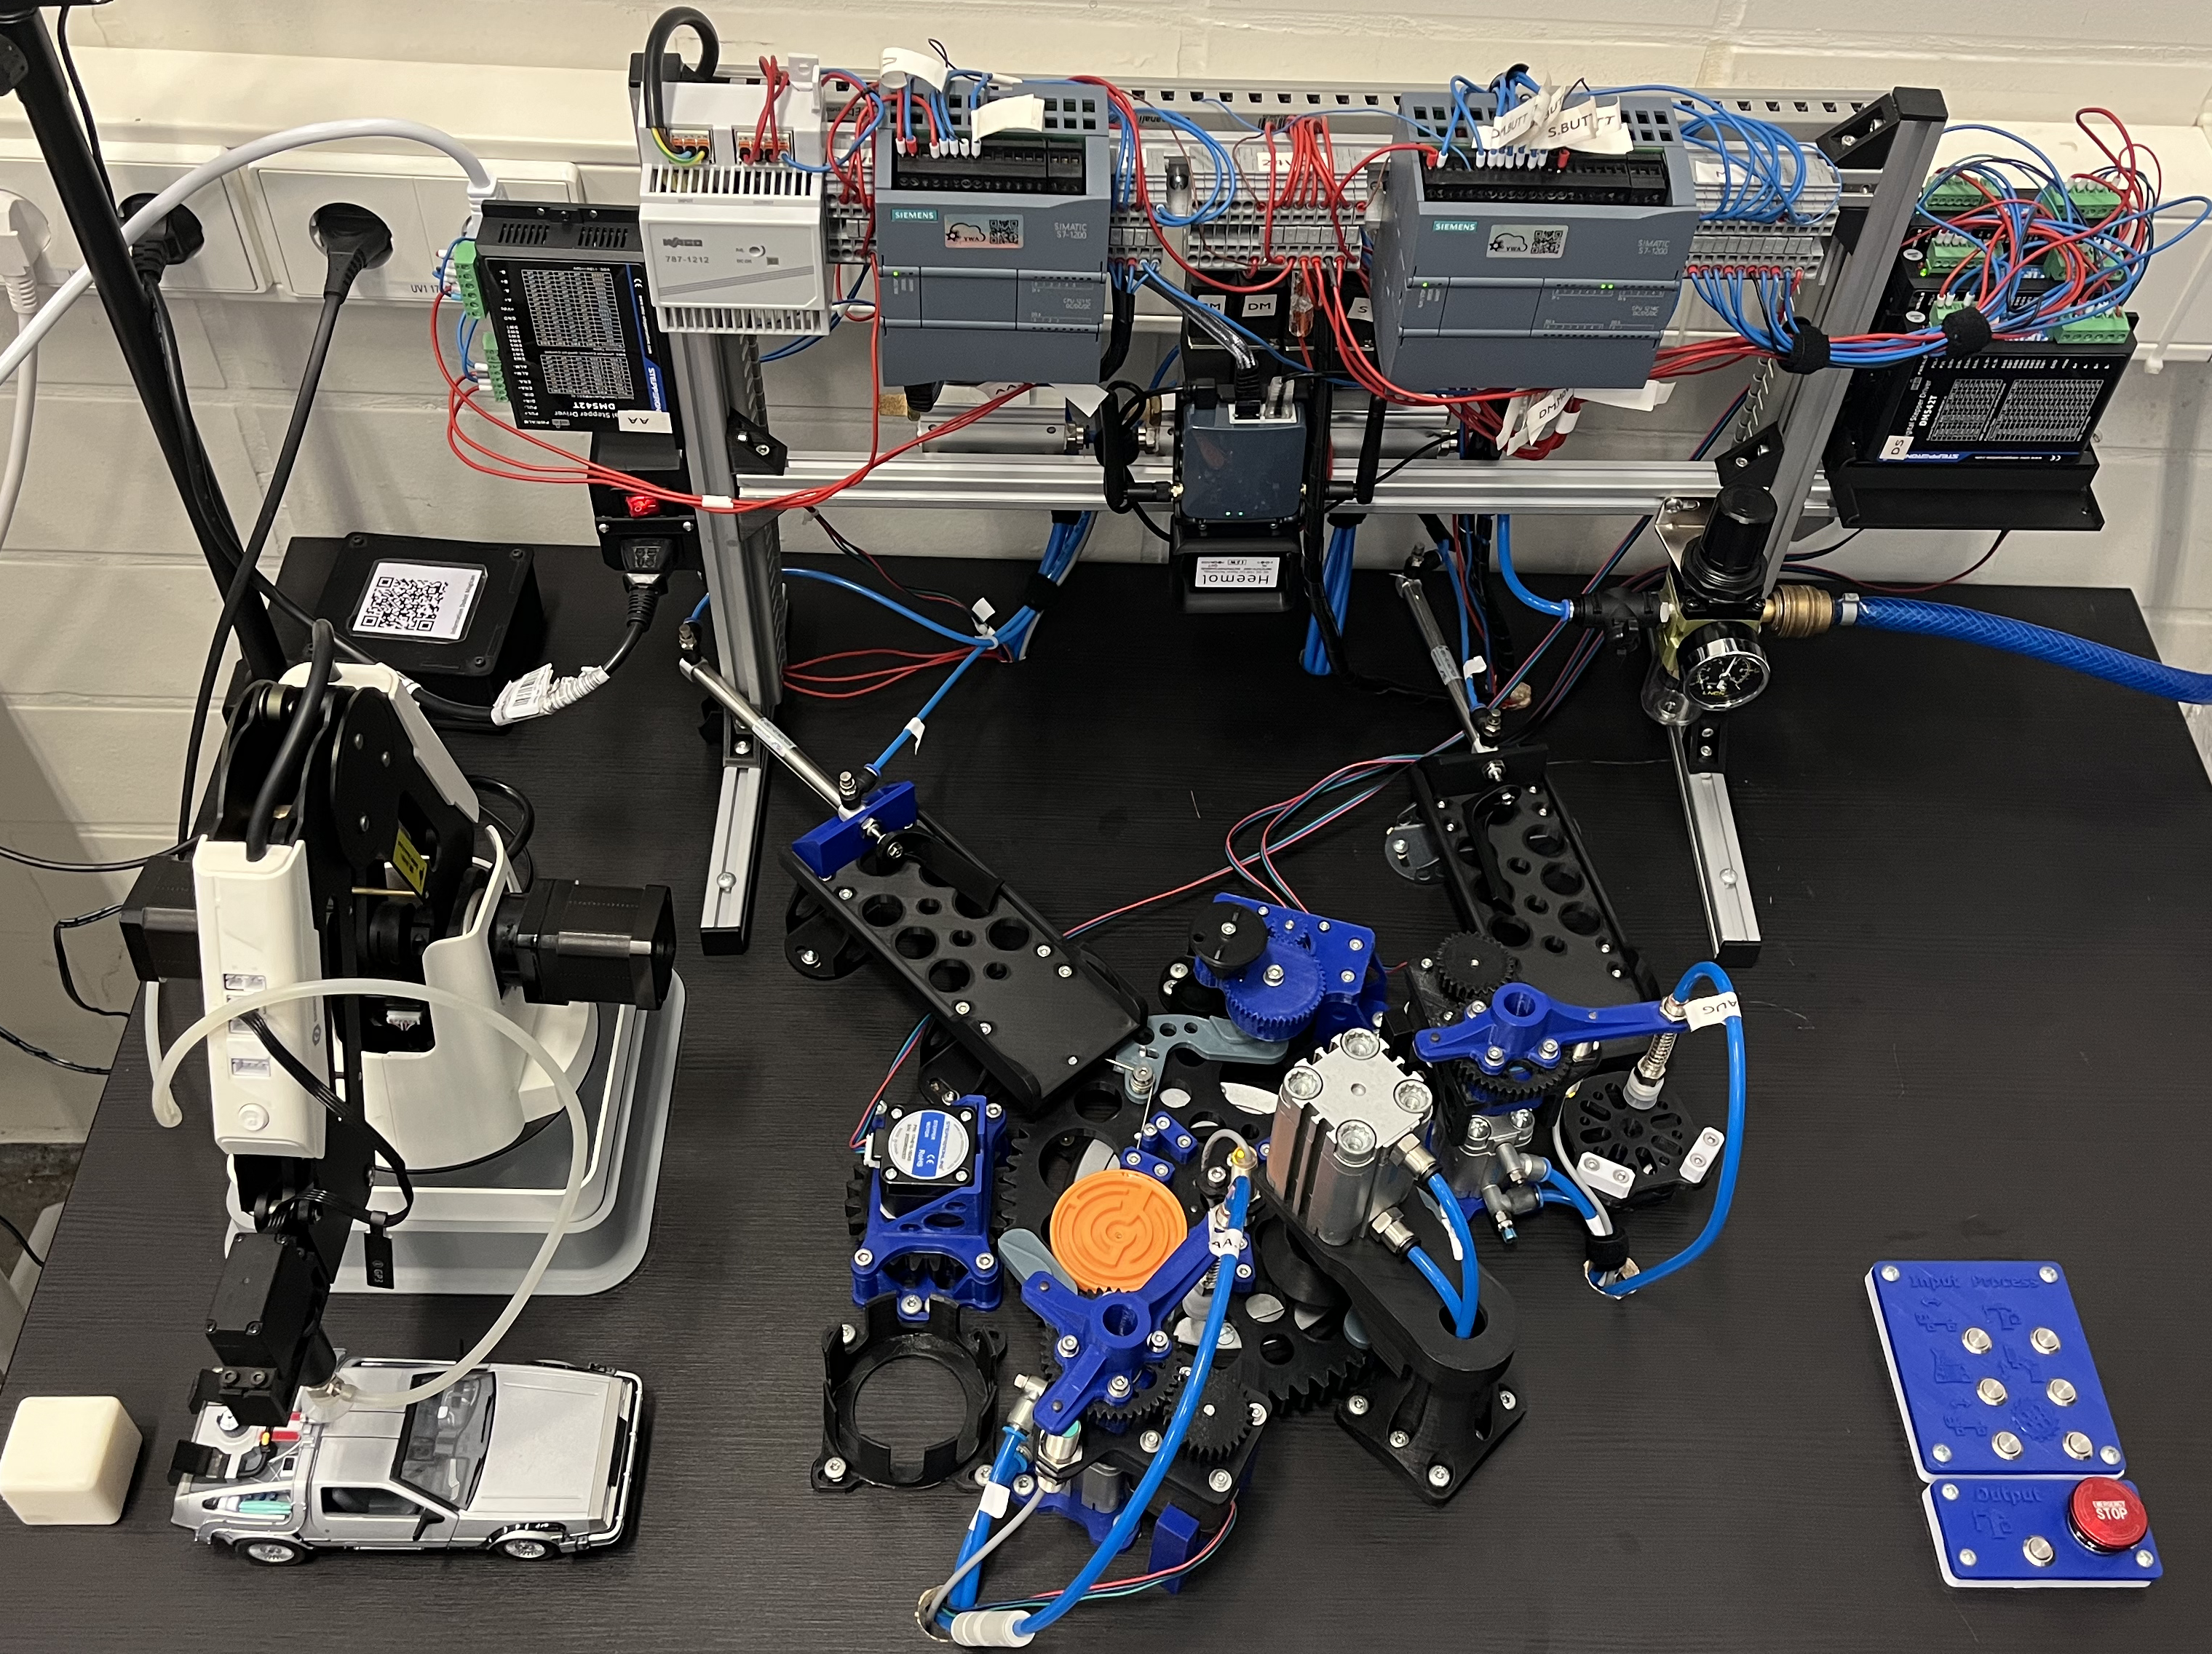
\includegraphics[width=1.25\linewidth]{Dobot und Mazerunner}}
    \caption{Finaler Tischaufbau aus Dobot Magician (links) und Maze-Runner-Anlage
        (rechts) im Labor für Produktentwicklung und Digitale Fabrik (LFP) der HsH.}
    \label{fig:dobot_mazerunner_tisch}
\end{figure}

\begin{longtable}{@{}clp{6.5cm}@{}}
\caption{Kennung, Komponente und Funktion im gemeinsamen Tischaufbau aus
    Abbildung~\ref{fig:dobot_mazerunner_tisch}, Kennzeichnung in der Abbildung
    folgt separat (1--19 Maze-Runner, A--E Dobot Magician)}
\label{tab:tischaufbau_komponenten}\\
\toprule
\textbf{Kennung} & \textbf{Komponente} & \textbf{Funktion} \\
\midrule
\endfirsthead
\toprule
\textbf{Kennung} & \textbf{Komponente} & \textbf{Funktion} \\
\midrule
\endhead
\multicolumn{3}{@{}l}{\textbf{Maze-Runner-Anlage}} \\
1 & Bodenmagazin-Station & Zuführung Bodenteile \\
2 & Deckelmagazin-Station & Zuführung Deckelteile \\
3 & Pufferstation & Zwischenlager Deckelmagazin \\
4 & Drehscheibe mit Kugelmagazin & Drehteller mit Kugelzuführung \\
5 & Erste Schwenkarmstation & Deckeltransfer zur Drehscheibe \\
6 & Presse & Fügt Boden und Deckel zusammen \\
7 & Ausgabeschwenkarmstation & Produktausgabe \\
8 & Steuer-Buttons & Manuelle Stationsbedienung \\
9 & Not-Aus-Knopf & Sicherheitsabschaltung \\
10 & Treiberplatinen & Schrittmotoransteuerung \\
11 & 230-V-Zufuhr & Netzanschluss \\
12 & 24-V-Netzteil & Ein-/Ausgangsversorgung \\
13 & Verteilerschienen & Elektrische Verteilung \\
14 & SPS~1 & Hauptsteuerung \\
15 & SPS~2 & Steuerung Ausgabeschwenkarmstation \\
16 & VPN-Router & Fernzugriff \\
17 & Magnetventile & Druckluftsteuerung \\
18 & Druckminderer & Reduzierung auf vier~Bar \\
19 & Druckluftzufuhr & Versorgung durch Laborkompressor \\
\multicolumn{3}{@{}l}{\textbf{Dobot Magician}} \\
A & Dobot Magician & Vierachsiger Roboterarm \\
B & Vakuumpumpe & Sauggreifer-Unterdruck \\
C & Sauggreifer & Endeffektor \\
D & DeLorean-Modellfahrzeug & Pick-and-Place-Objekt \\
E & Schutzkappe & Aufsetzbauteil \\
\bottomrule
\end{longtable}

\subsection{Anforderungsanalyse}
\label{subsec:anforderungsanalyse}
Eine tabellarische Anforderungsanalyse gliedert Projektziele in überprüfbare
Einzelanforderungen.
Die Klassifizierung in Festforderungen, die vollständig umgesetzt werden müssen, und
Wunschforderungen, die bei verbleibenden Ressourcen angestrebt werden, entspricht
ingenieurwissenschaftlichem Vorgehen.
Die Nummerierung der Anforderungen schafft im weiteren Verlauf der Arbeit eine
eindeutige Rückverfolgbarkeit.
Im Folgenden sind die Anforderungstabellen der beiden Digitalen Zwillinge aufgeführt.
Das Kürzel MR steht für Maze-Runner, DM steht für Dobot Magician.

\begin{table}[H]
\centering
\caption{Anforderungen an den Digitalen Zwilling des Maze-Runner}
\label{tab:anf_mazerunner}
\begin{tabularx}{\textwidth}{lXc}
\toprule
\textbf{Nr.} & \textbf{Anforderung} & \textbf{Klasse} \\
\midrule
MR-1 & Gesamte Maze-Runner-Anlage in Betrieb nehmen                                      & Festforderung \\
MR-2 & CAD-Modell der Maze-Runner-Anlage in NVIDIA Isaac Sim konvertieren und hierarchisch sortieren & Festforderung \\
MR-3 & Anlage an die Netzwerkinfrastruktur der HSRM zur Nutzung per Digital Twin App anpassen      & Festforderung \\
MR-4 & Bewegungsachsen mit PhysX in NVIDIA Isaac Sim simulieren                                    & Festforderung \\
MR-5 & Reale Anlage über die Digital Twin App der HSRM steuern                                     & Festforderung \\
MR-6 & Digitales Modell bei ausgehendem OPC-UA-Befehl ebenfalls steuern               & Festforderung \\
MR-7 & Schritt-für-Schritt-Reproduzierbarkeitsdokumentation erstellen                & Festforderung \\
MR-8 & Geänderte Steuerungswerte der SPS per MQTT empfangen                            & Wunsch \\
MR-9 & Anlage in VR mit der Meta Quest~3 demonstrieren                                 & Wunsch \\
\bottomrule
\end{tabularx}
\end{table}

\begin{table}[H]
\centering
\caption{Anforderungen an den Digitalen Zwilling des Dobot Magician}
\label{tab:anf_dobot}
\begin{tabularx}{\textwidth}{lXc}
\toprule
\textbf{Nr.} & \textbf{Anforderung} & \textbf{Klasse} \\
\midrule
DM-1 & CAD-Modell des Dobot Magician in NVIDIA Isaac Sim konvertieren               & Festforderung \\
DM-2 & Bidirektionalen Datenfluss via ROS\,2 herstellen                           & Festforderung \\
DM-3 & Pick-and-Place-Szenario in der Simulation ausführen                        & Festforderung \\
DM-4 & Erstellung des Digitalen Zwillings als technische Anleitung dokumentieren  & Festforderung \\
\bottomrule
\end{tabularx}
\end{table}

\subsection{Toolkette}
Die Erstellung der Digitalen Zwillinge folgte einem mehrstufigen Workflow.
Tabelle~\ref{tab:toolkette} stellt die eingesetzten Werkzeuge beider Anlagen gegenüber.

\begin{table}[H]
\centering
\caption{Toolkette der Digitalen Zwillinge im Vergleich}
\label{tab:toolkette}
\begin{tabularx}{\linewidth}{p{3.3cm}XX}
\toprule
\textbf{Schritt} & \textbf{Maze-Runner} & \textbf{Dobot Magician} \\
\midrule
Modell\-beschaffung
  & Maze-Runner-CAD-Baugruppe der HSRM
  & Einzelteile und URDF-basierte Baugruppe vom Hersteller \\
Konstruktion
  & Autodesk Inventor, Bambu Studio
  & Autodesk Inventor, Zoo Studio, Bambu Studio \\
Import und Szenen\-aufbau
  & STEP-Import, Konvertierung nach OpenUSD in NVIDIA Isaac Sim
  & URDF-Import in NVIDIA Isaac Sim \\
Kinematik\-definition
  & Ordner\-struktur mit \texttt{\_fix}/\texttt{\_move} und Gelenk\-definition
  & Artikulationsbaum via URDF \\
Steuerungs\-schicht
  & TIA Portal V17 (SPS-Programmierung, OPC-UA-Server), UaExpert (OPC-UA-Knotenbrowser)
  & Interne Steuerung des Dobot Magician, COM-Port (USB~3.0) \\
Extension\-entwicklung
  & Visual Studio Code, mit KI-Werkzeugen (s.\ Anhang~\ref{anhang:ki})
  & Visual Studio Code, mit KI-Werkzeugen (s.\ Anhang~\ref{anhang:ki}) \\
Versions\-kontrolle
  & Git, GitHub-Verzeichnis, VS~Code GitHub-Extension
  & Git, GitHub-Verzeichnis, VS~Code GitHub-Extension \\
Kommunikations\-anbindung
  & OPC-UA via open62541, MQTT via paho-mqtt~1.6.1
  & ROS\,2 Humble, \emph{pydobot} (USB~3.0/COM-Port), interne ROS\,2-Extension von NVIDIA Isaac Sim \\
Validierung
  & Funktionsprüfung an der Maze-Runner-Anlage im Labor, korrektes Verhalten der NVIDIA Isaac Sim Szene
  & Funktionsprüfung mit realer Hardware im Pick-and-Place-Szenario, korrektes Verhalten der NVIDIA Isaac Sim Szene \\
Dokumentation
  & Schritt-für-Schritt-Reproduzierbarkeitsdokumentation (PowerPoint-Folien)
  & Technische Dokumentation (PDF, \LaTeX) \\
\bottomrule
\end{tabularx}
\end{table}

\subsection{Anlage 1: Rundtakttisch \enquote{Maze-Runner}}

Die Maze-Runner-Anlage wurde an der Hochschule RheinMain (HSRM) für Lehrzwecke der industriellen Automatisierung entwickelt~\cite{wang2024mazerunner}.
Ihre sieben Stationen sind in drei Trainingslevel gegliedert, die im Lehrbetrieb zunächst einzeln behandelt werden, bevor sie zu dem in Abbildung~\ref{fig:mazerunner_aktorik} gezeigten gemeinsamen Produktionssystem zusammengeführt werden.
Der begleitende Kurs behandelt dabei von der CAD-Konstruktion und dem 3D-Druck der Bauteile bis hin zur SPS-Programmierung mit TIA und der Anbindung an eine Cloud-Plattform~\cite{dtcenter_trainingslevel}.
Über diese Cloud-Plattform, die \emph{Digital Twin App}, wird die Anlage in einer hochschulübergreifenden Vorlesung für die teilnehmenden Partnerhochschulen, die vorwiegend aus dem asiatischen Raum stammen, in einem gemeinsamen Dashboard zugänglich gemacht.
Über einen Kamera-Livestream können die teilnehmenden Hochschulen dabei live mitverfolgen, was gerade an der realen Anlage sowie am zugehörigen Digitalen Zwilling in NVIDIA Isaac Sim geschieht (vgl.\ Abschnitt~\ref{subsubsec:mazerunner_sps}).
Im Folgenden werden Anlagenaufbau, Geometrie, Kinematik, Inbetriebnahme und Netzwerkarchitektur sowie die Entwicklung der NVIDIA Isaac Sim Extension beschrieben.

\subsubsection{Beschreibung der Anlage}
Das von der Anlage gefertigte Produkt ist ein rundes Labyrinth aus FDM-gedrucktem Kunststoff, wie in Abbildung~\ref{fig:mazerunner_produkt} zu sehen ist.
In das Labyrinth wird eine Metallkugel mit einem Durchmesser von drei Millimetern eingelegt, anschließend wird eine Plexiglasplatte aufgelegt und verpresst.
Vom Durchlaufen der Kugel durch das Labyrinth leitet sich der Name Maze-Runner ab.

Die sieben Stationen der Anlage sind in Form eines Rundtakttisches aufgebaut.
Dabei kommt neben elektrischer auch pneumatisch angetriebene Aktorik zum Einsatz.
Dazu zählen Pneumatikzylinder, die Schieber antreiben, oder die pneumatische Presse.
Zudem lässt sich Druckluft auch über einen Vakuumejektor zum Betrieb eines Sauggreifers nutzen, wobei die Druckluft über pneumatische Magnetventile gesteuert wird.
Ergänzend kommen rein mechanische Komponenten wie federangetriebene Fixierarme zum Einsatz, welche das Werkstück in der Halterung auf der Drehscheibe fixieren, wie in Abbildung~\ref{fig:mazerunner_produkt} dargestellt.

\begin{figure}[H]
    \centering
    \begin{minipage}[t]{0.56\linewidth}
        \centering
        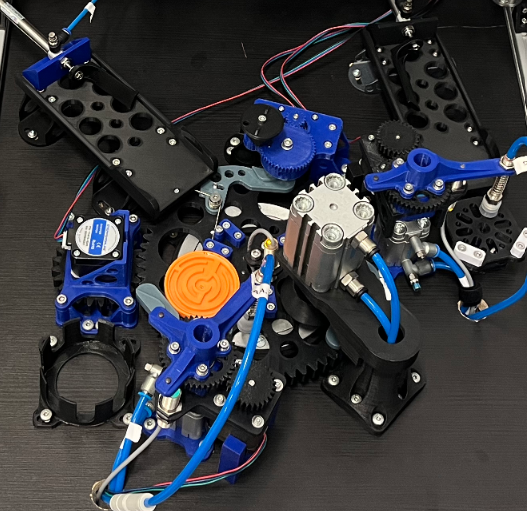
\includegraphics[height=8.6cm]{Mazerunner_Aktorik}
        \caption{Aktorik der Maze-Runner-Anlage.}
        \label{fig:mazerunner_aktorik}
    \end{minipage}
    \hfill
    \begin{minipage}[t]{0.40\linewidth}
        \centering
        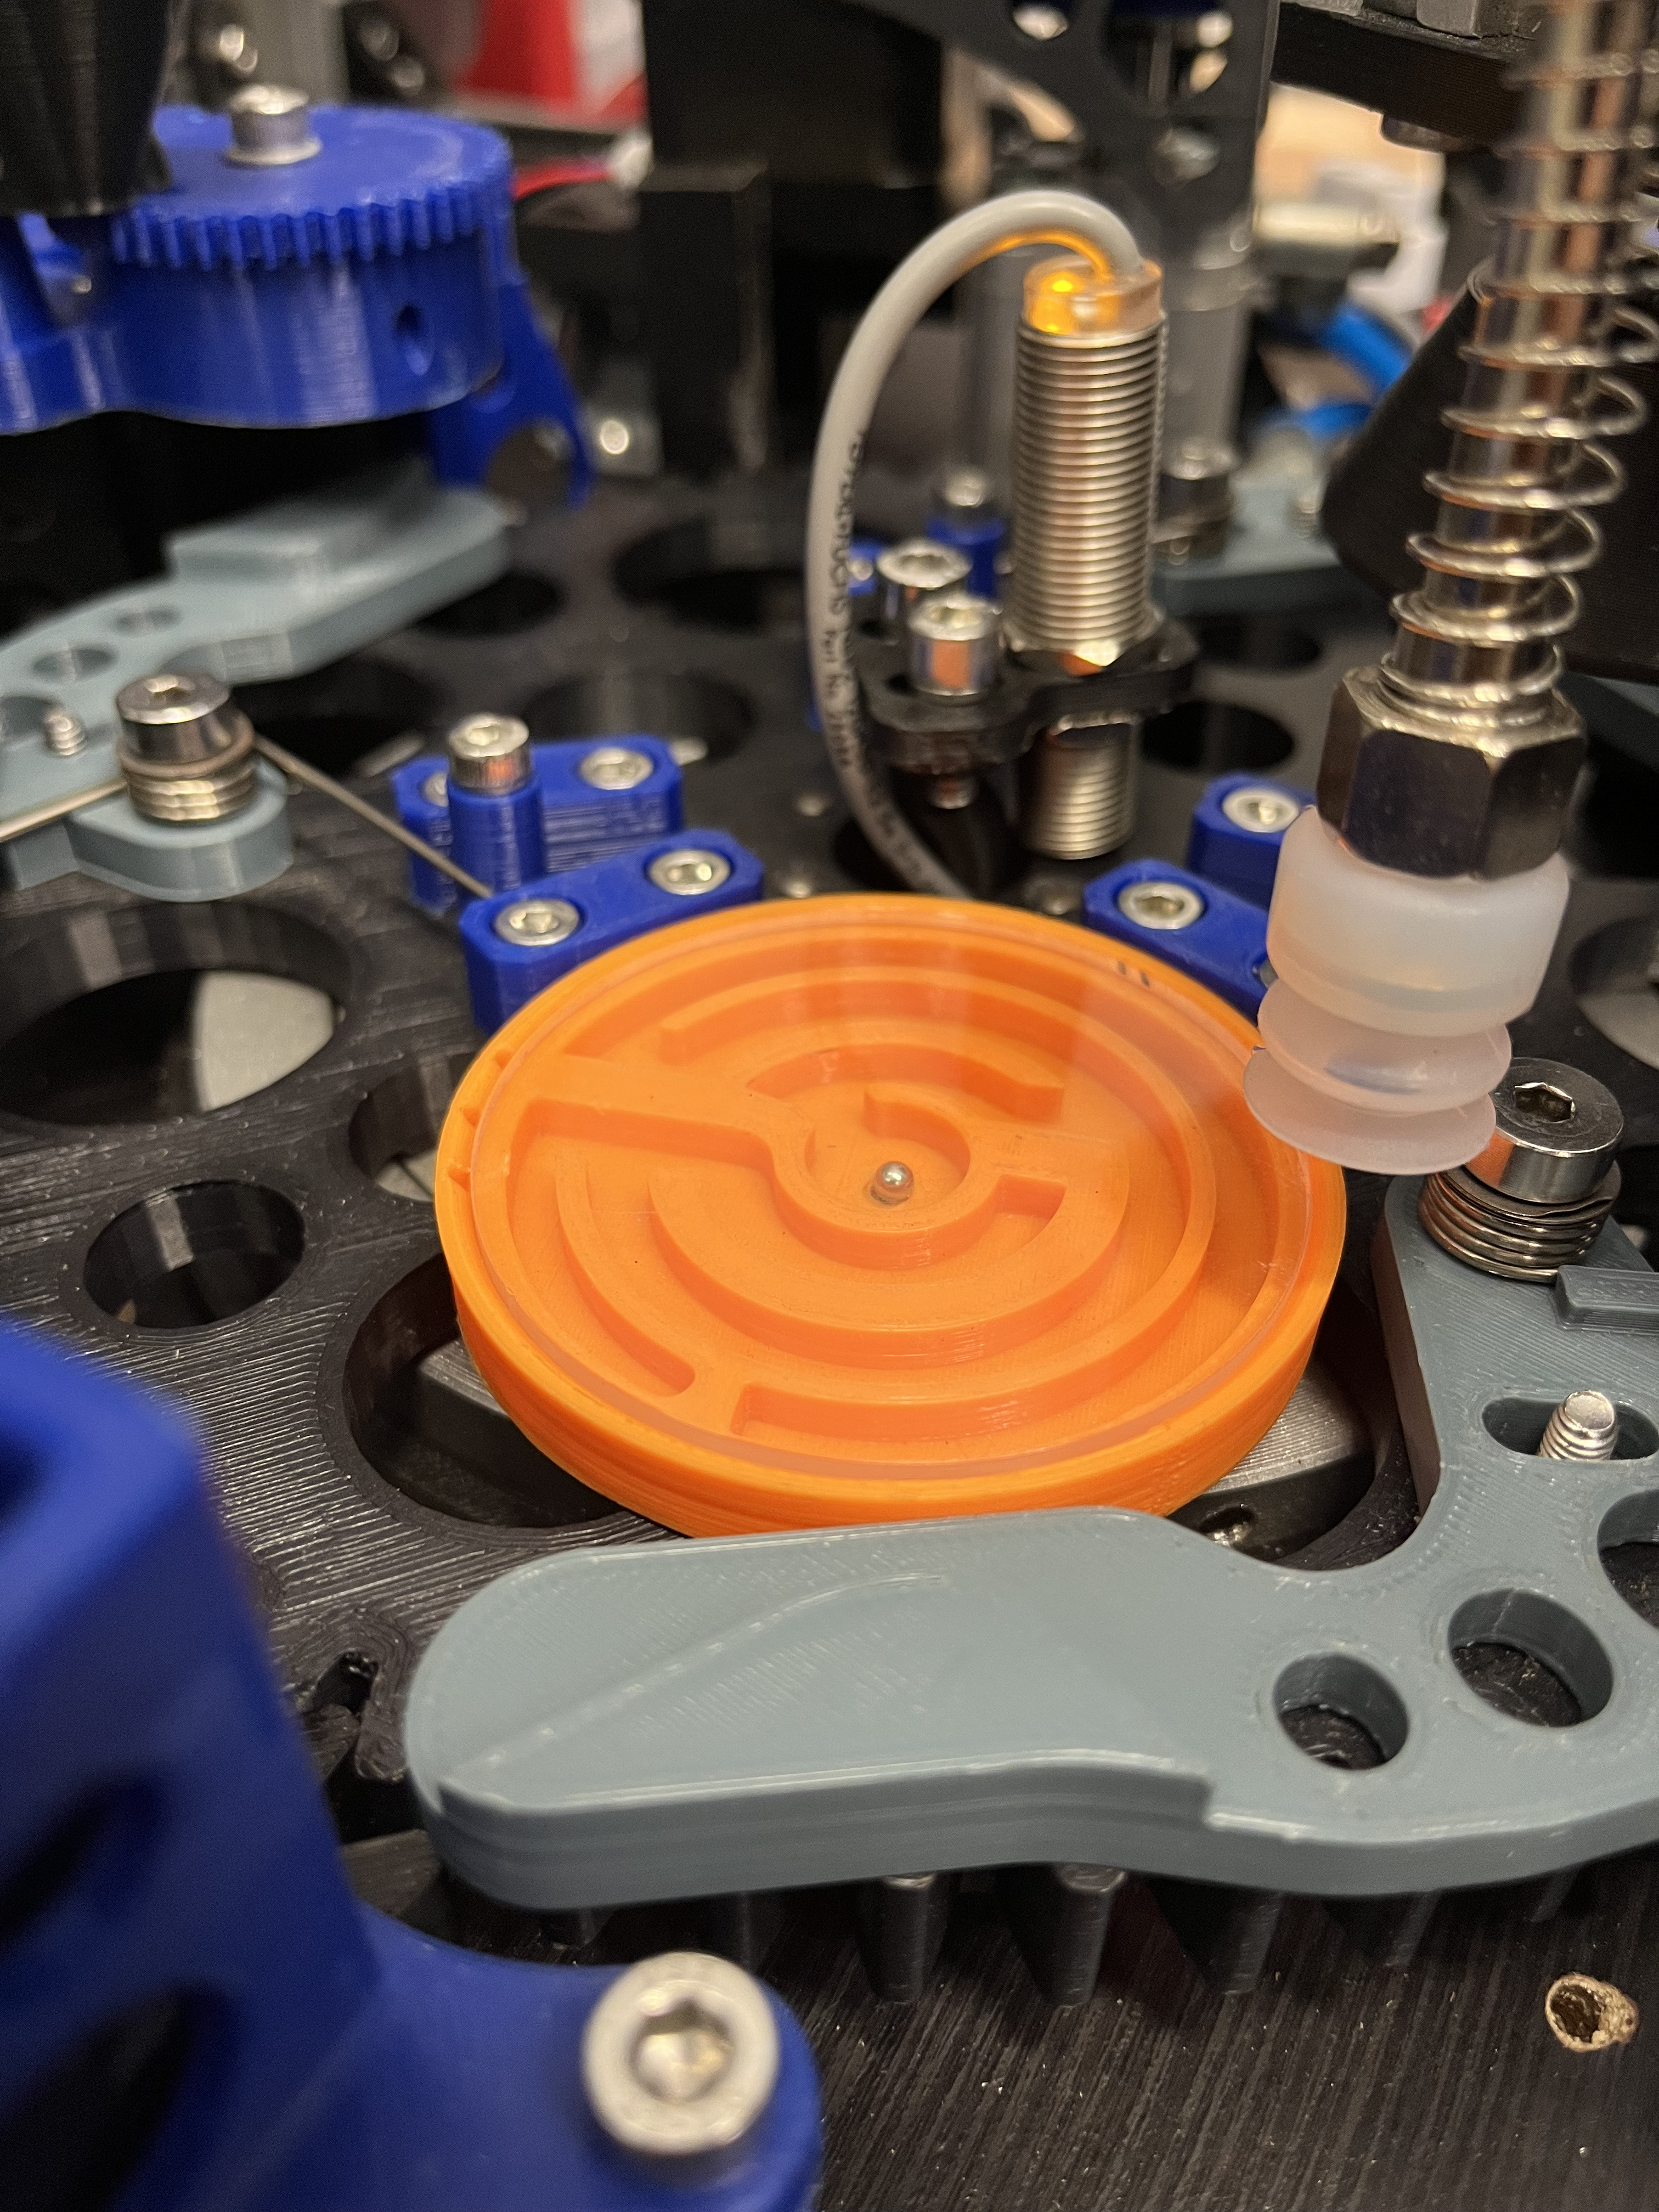
\includegraphics[height=8.6cm]{MazeRunnerProdukt}
        \caption{Produkt der Maze-Runner-Anlage, auf der Drehscheibe fixiert.}
        \label{fig:mazerunner_produkt}
    \end{minipage}
\end{figure}

\textbf{Das erste Level} bildet die \enquote{Magazinstation} und beinhaltet die Inbetriebnahme eines Pneumatikzylinders, der in der Anlage als Bodenmagazin-Station und als Deckelmagazin-Station vorkommt.
Diese Stationen speichern die Produktkomponenten über Turmmagazine und führen sie über pneumatisch betriebene Schieber der Drehscheibe und der Pufferstation zu.
Die Bauteile wurden als CAD-Modell konstruiert, im FDM-Verfahren gefertigt und auf einem gemeinsamen Montagetisch montiert~\cite{wang2024mazerunner}.
Abbildung~\ref{fig:maze_l1} zeigt eine dieser Versorgungsstationen mit dem zylindrischen Bauteilmagazin und dem Pneumatikzylinder, der den Schieber antreibt.
Als Aktoren kommen Magnetventile sowie Pneumatikzylinder zum Einsatz~\cite{wang2024mazerunner}.

\textbf{Das zweite Level} bildet die Station \enquote{Drehscheibe mit Kugelmagazin} und ergänzt die Anlage um eine schrittmotorgesteuerte Drehscheibe sowie ein Kugelmagazin.
Der zentrale Drehteller wird über einen Schrittmotor mit Zahnradübertragung angetrieben, ein induktiver Näherungsschalter erfasst die Drehteller-Position und übergibt das Signal an die SPS.
Die SPS dreht den Drehteller so lange, bis der induktive Sensor auslöst und die Zielposition damit erreicht ist.
Das Kugelmagazin wird ebenfalls über einen Schrittmotor gesteuert, wobei das kugeltreibende Zahnrad stets eine volle Umdrehung ohne Sensorik ausführt.
Abbildung~\ref{fig:maze_l2} zeigt die Antriebseinheit mit dem Zahnrad der Drehscheibe sowie das trichterförmige Kugelmagazin~\cite{wang2024mazerunner}.

\textbf{Das dritte Level} bildet die \enquote{Ausgabeschwenkarmstation} und vervollständigt die Produktionslinie um zwei Schwenkarmstationen sowie eine Presse.
Die erste Schwenkarmstation saugt den Deckel des Deckelmagazins über einen Sauggreifer aus der Pufferstation an und legt ihn auf das Bodenmagazin auf der Drehscheibe, wo die pneumatische Presse beide Komponenten anschließend zusammenfügt.
Die zweite Schwenkarmstation, die Ausgabeschwenkarmstation, überführt das fertige Produkt vom Drehteller zum Ausgabeteillager.
Abbildung~\ref{fig:maze_l3} zeigt die Ausgabeschwenkarmstation, deren Schrittmotor die Drehbewegung des Arms ausführt, während ein Pneumatikzylinder die vertikale Hubbewegung übernimmt~\cite{wang2024mazerunner}.

\begin{figure}[H]
    \centering
    \begin{subfigure}[t]{0.32\linewidth}
        \centering
        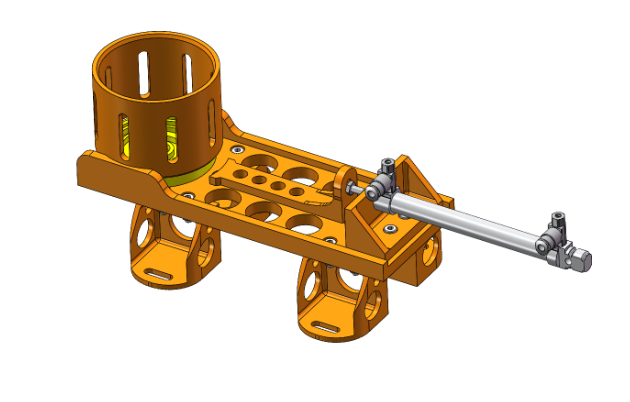
\includegraphics[width=\linewidth]{MazerunnerLevel1.png}
        \caption{Level 1 (Magazinstation)}
        \label{fig:maze_l1}
    \end{subfigure}
    \hfill
    \begin{subfigure}[t]{0.32\linewidth}
        \centering
        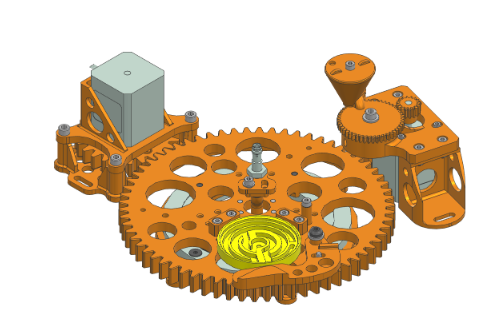
\includegraphics[width=\linewidth]{Mazerunner level2}
        \caption{Level 2 (Drehscheibe mit Kugelmagazin)}
        \label{fig:maze_l2}
    \end{subfigure}
    \hfill
    \begin{subfigure}[t]{0.32\linewidth}
        \centering
        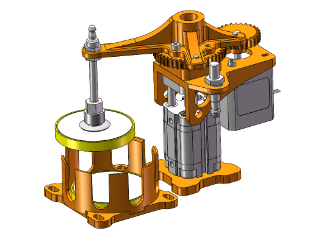
\includegraphics[width=\linewidth]{Mazerunnerlevel3}
        \caption{Level 3 (Ausgabeschwenkarmstation)}
        \label{fig:maze_l3}
    \end{subfigure}
    \caption{Die drei Trainingslevel der Maze-Runner-Anlage~\cite{wang2024mazerunner}}
    \label{fig:mazerunner_level}
\end{figure}

Die Anlage wird von zwei Siemens-SPS der S7-1200-Serie gesteuert, wobei eine SPS ausschließlich für die in Abbildung~\ref{fig:maze_l3} dargestellte Ausgabeschwenkarmstation eingesetzt wird.
Grund dafür sind die ausgelasteten Ein- und Ausgänge der Haupt-SPS.
Beide Einheiten betreiben einen OPC-UA-Server gemäß DIN~EN~IEC~62541 auf Port~4840, über den Sensor- und Aktorvariablen bereitgestellt werden~\cite{wang2024mazerunner,iec62541}.
Auf Basis der Dokumentation vorangegangener Maze-Runner-Projekte der HSRM~\cite{wang2024mazerunner} wurden Aufbau, Verschaltung, Sensorik und Aktorik in einer Schnittstellenmatrix zusammengefasst (vgl.\ Anhang~\ref{anhang:schnittstellen}).

\subsubsection{Geometrie und USD-Konvertierung}
Ausgangspunkt der geometrischen Modellierung ist das vom Kooperationspartner bereitgestellte CAD-Modell im STEP-Format.
Über den Isaac-Sim-STEP-Importer wird es in das Format OpenUSD überführt, wobei Baugruppenhierarchien als USD-\emph{Xforms} und Einzelteile als \emph{Mesh}-Primitives übertragen werden.
Abbildung~\ref{fig:mazerunner_isaac} zeigt das fertige Modell in der Isaac-Sim-Arbeitsumgebung.
Im Stage-Baum ist die hierarchische Ordnerstruktur der Stationen sichtbar.
Bauteile sind in \texttt{\_fix}- und \texttt{\_move}-Unterordner gegliedert, und das zugehörige Gelenk ist im selben Ordner abgelegt.
Am Beispiel des Deckelmagazins ist ein \emph{primPath} markiert, der als Adresse innerhalb der USD-Hierarchie fungiert und alle beweglichen Teile dieser Station referenziert.

\begin{figure}[H]
    \centering
    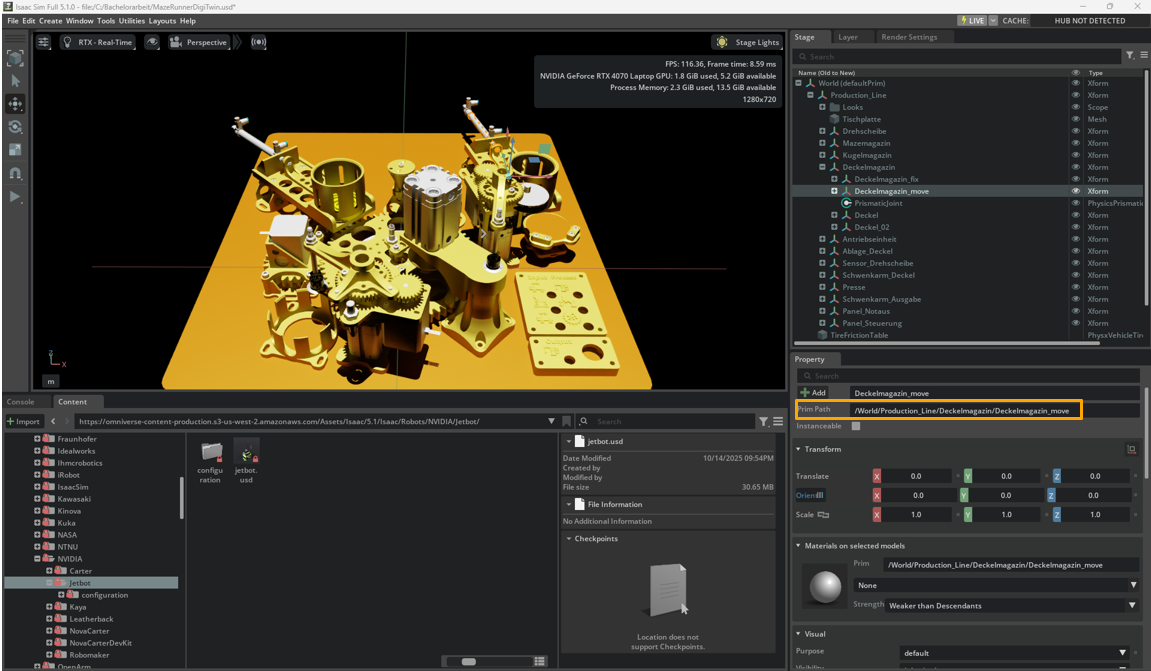
\includegraphics[width=\linewidth]{Mazerunner_in_Isaac_Sim}
    \caption{OpenUSD-Modell des Maze-Runners in NVIDIA Isaac Sim (Viewport, Stage-Baum und Property-Panel).}
    \label{fig:mazerunner_isaac}
\end{figure}

\subsubsection{Kinematik und Physik in NVIDIA Isaac Sim}
Die kinematische Struktur des Rundtakttisches wird in NVIDIA Isaac Sim durch PhysX-\emph{Articulations} abgebildet.
Der zentrale Drehteller wird als \emph{Revolute Joint} parametriert, die pneumatischen Schieber als \emph{Prismatic Joints}.
Die Antriebsparameter Steifigkeit und Dämpfung legen das dynamische Verhalten der Gelenke fest.
Eine höhere Steifigkeit bewirkt, dass der Antrieb die Zielposition mit größerer Kraft ansteuert, während die Dämpfung für sanfteres Anfahren und Abbremsen sorgt.
Massen und Trägheitsmomente wurden automatisch berechnet, Reibungskoeffizienten wurden auf den Isaac-Sim-Standardwerten belassen.
Die Parametrierung wurde durch Abgleich mit dem realen Anlagenverhalten verifiziert~\cite{nvidia_physx}.

Besondere Sorgfalt erfordert die Modellierung verschachtelter Gelenke, wie sie am Schwenkarm-Deckel auftreten.
Dieser vereint ein Drehgelenk und ein Schubgelenk in einer kinematischen Kette.
Die USD-Baugruppe wird hierzu in die Untergruppen \texttt{Schwenkarm-Deckel\_fix} und \texttt{Schwenkarm-Deckel\_move} gegliedert.
\texttt{\_fix} beinhaltet alle Teile, die nicht bewegt werden, \texttt{\_move} beinhaltet zwei weitere Unterordner für die translatorischen und die rotatorischen Teile.
Der translatorische Unterordner beinhaltet die Aufbaukonstruktion abzüglich der sich drehenden Teile, während der rotatorische Unterordner ausschließlich die sich drehenden Teile beinhaltet.
Die Gelenke sind im allgemeinen \texttt{\_move}-Ordner abgelegt, wie Abbildung~\ref{fig:verschachtelte_gelenke} zeigt.

\begin{figure}[H]
    \centering
    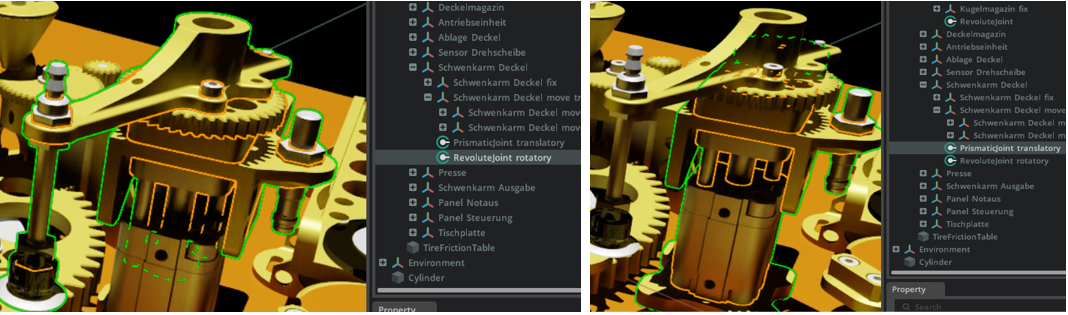
\includegraphics[width=\linewidth]{verschachtelte_Gelenke_am_Schwenkarm}
    \caption{Verschachtelte Gelenke am Schwenkarm-Deckel: \emph{RevoluteJoint~rotatory} (links) und \emph{PrismaticJoint~translatory} (rechts) mit Kollisionskonturen (grün).}
    \label{fig:verschachtelte_gelenke}
\end{figure}

\subsubsection{SPS-Konfiguration}
\label{subsubsec:mazerunner_steuerung_anwendung}

Bevor die Omniverse-Extension einzelne SPS-Variablen adressieren kann, müssen zunächst deren Node-IDs im OPC-UA-Adressraum der Anlage bekannt sein.
Die Siemens-SPS stellt sämtliche für den Digitalen Zwilling relevanten Signale als OPC-UA-fähige Knoten bereit, die sich mit dem Browsing-Werkzeug UaExpert auslesen lassen.
Abbildung~\ref{fig:uaexpert} zeigt einen Ausschnitt der auf diese Weise identifizierten Knoten mit Server-Adresse, Node-ID, Knotenpfad und Anzeigename.
Jede identifizierte Node-ID wird im \emph{DigitalTwinService} hinterlegt und lässt sich anschließend über einen REST-API-Aufruf per HTTP ansteuern und abfragen, worüber die Omniverse-Extension im weiteren Verlauf lesend und schreibend auf die SPS zugreift.

\begin{figure}[H]
    \centering
    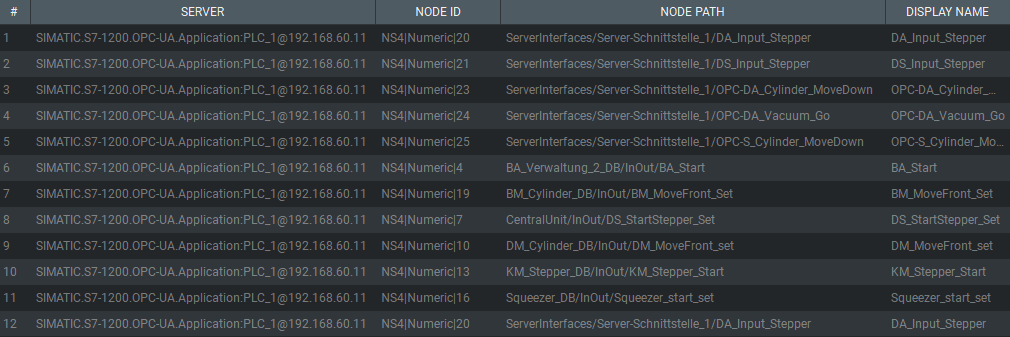
\includegraphics[width=\linewidth]{UAExpert}
    \caption{UaExpert-Knotenbrowser mit den von der Siemens-SPS bereitgestellten OPC-UA-Knoten (Server-Adresse, Node-ID, Knotenpfad, Anzeigename).}
    \label{fig:uaexpert}
\end{figure}

Die Knoten eins bis fünf werden als solche nicht direkt von der Extension verwendet.
Die hier hinterlegten Variablen werden stattdessen innerhalb der SPS von der Routine \texttt{BA\_Start} angesprochen, welche das Ansaugen und Ablegen des Deckels sowie die Steuerung des Schrittmotors, des Zylinders und des Schwenkarms verwaltet.
Beim Schrittmotor steuert \texttt{BA\_Start} dabei sowohl dessen Drehrichtung als auch die durch den induktiven Sensor ausgelöste Beendigung der Drehbewegung.
Die Extension arbeitet dabei ausschließlich mit dem Knoten \texttt{BA\_Start}.
Die weiteren Knoten sieben bis elf sind äquivalent zu den Tastern am Tisch.

Im Folgenden wird auf die Projektstruktur des TIA-Portal-V17-Projekts \texttt{Maze\_1214+1211} eingegangen, welches die beiden SPS-Bausteine unter \texttt{PLC\_1} und \texttt{PLC\_2} beinhaltet.
Abbildung~\ref{fig:tia_portal} zeigt die aufgeklappte Projektstruktur von \texttt{PLC\_1}, die den Inhalt der Main-Methode, welche in Netzwerken programmiert ist, sowie die OPC-UA-Schnittstelle umfasst, in der die Variablen definiert sind, die über einen Client am Server abgefragt werden können.
Jedes Netzwerk der Main-Methode wird dauerhaft abgefragt und setzt bei erfüllter Eingangsbedingung die jeweils aufgeführte Variable.
An der Programmierung selbst wurde dabei nichts verändert, TIA Portal diente lediglich dem tieferen Anlagenverständnis sowie der Einbindung der SPS in das Netzwerk der Hochschule RheinMain.

\begin{figure}[H]
    \centering
    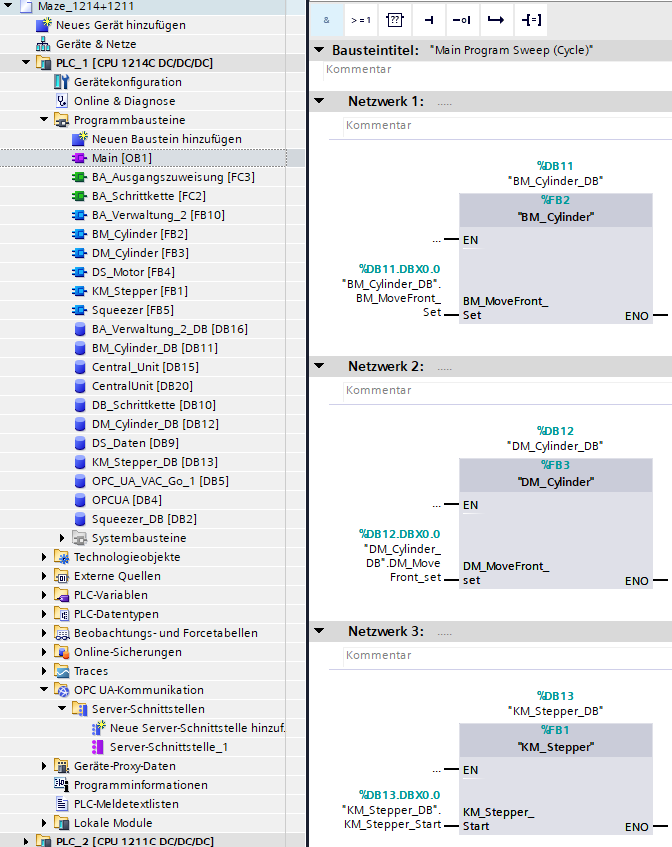
\includegraphics[width=\linewidth]{TIA_Portal_V17}
    \caption{TIA Portal V17 mit Programmbausteinen und OPC-UA-Serverschnittstelle des Maze-Runner-SPS-Projekts.}
    \label{fig:tia_portal}
\end{figure}

\subsubsection{Aufbau der Omniverse-Extension}
\label{subsubsec:mazerunner_extension}

Im Folgenden wird gezeigt, wie auf Grundlage der Inhalte der vorangegangenen drei Abschnitte eine Omniverse-Extension aufgebaut wird.
An die Isaac-Sim-Oberfläche wurde ein Human-Machine-Interface (HMI) angedockt, das die Interaktion sowie die Diagnose und Aufbereitung der Ereignisse des Digitalen Zwillings darstellt.
Abbildung~\ref{fig:mazerunner_extension} zeigt die Isaac-Sim-Oberfläche mit dem geöffneten Maze-Runner-HMI.
Programmiert wurden das HMI sowie das dahinterstehende Backend innerhalb einer modularen Omniverse-Extension im \emph{Omniverse Kit Extension Framework}~\cite{nvidia_kit_extensions_advanced}.
Im Folgenden wird darauf eingegangen, welche Bestandteile die Extension hat, wie diese zusammenarbeiten und wie sie erstellt wurden.

\begin{figure}[H]
    \centering
    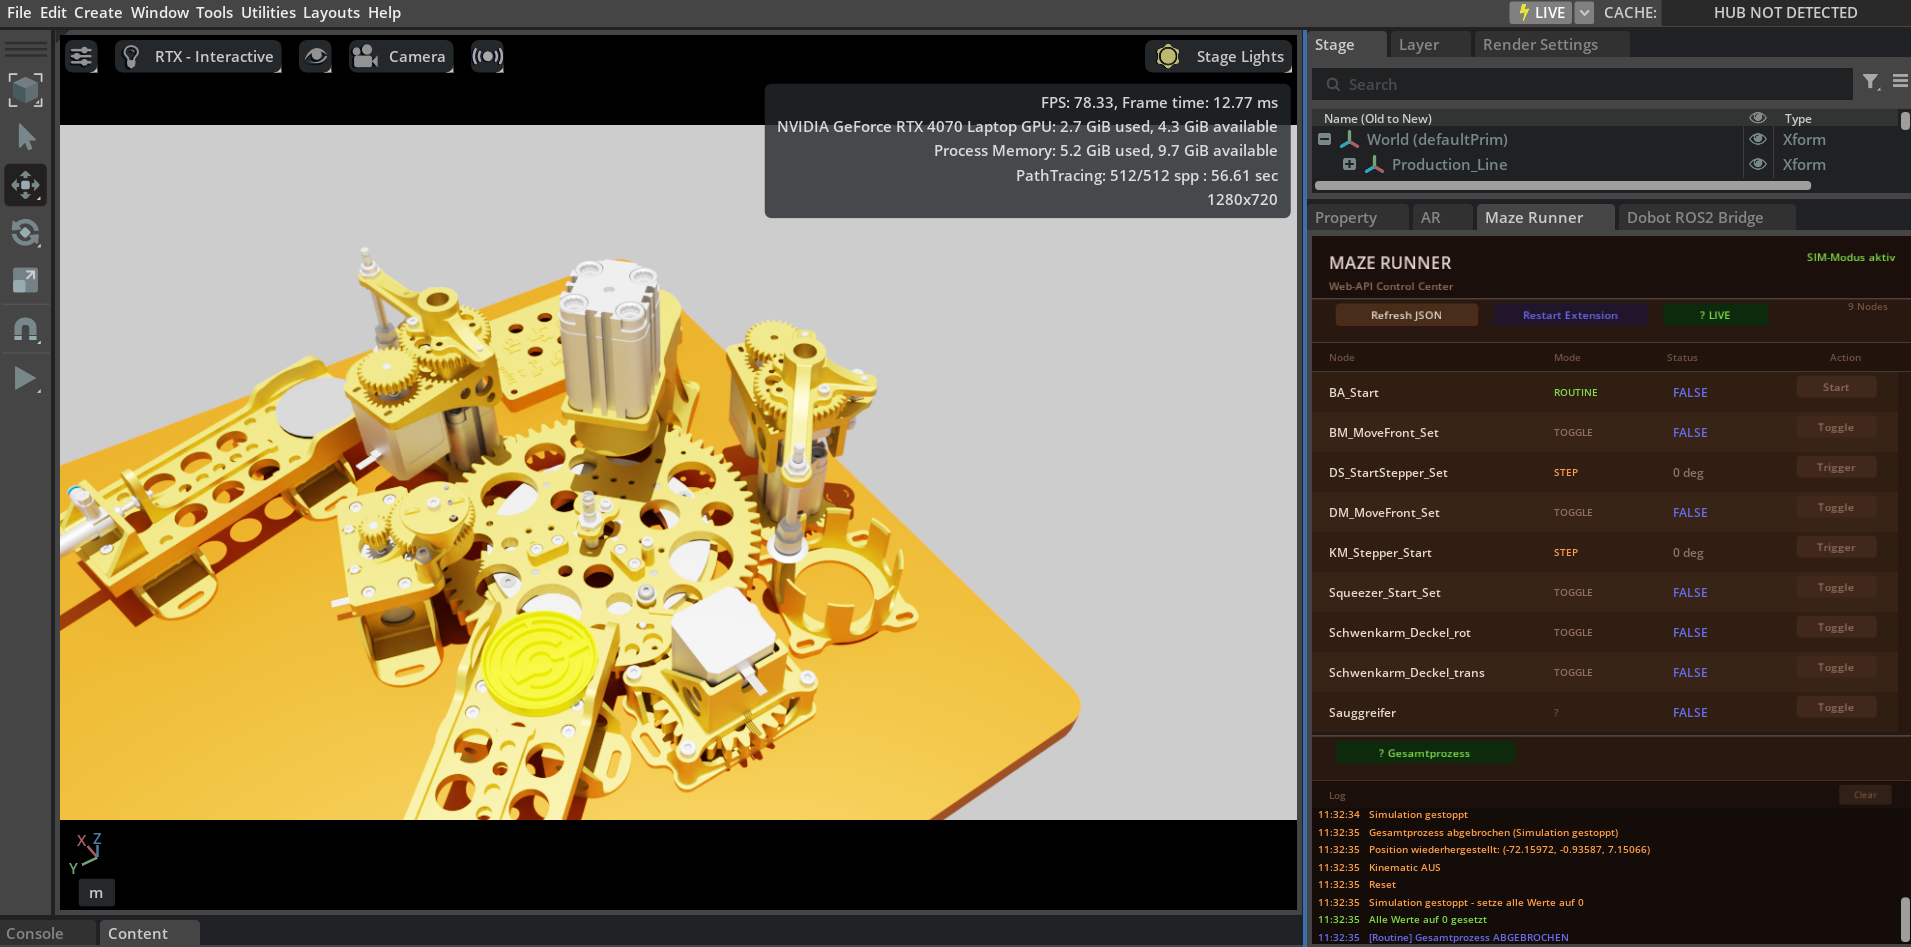
\includegraphics[width=\linewidth]{MazerunnerExtension}
    \caption{Benutzeroberfläche der Omniverse-Extension des Maze-Runner-Digitalen-Zwillings in NVIDIA Isaac Sim.}
    \label{fig:mazerunner_extension}
\end{figure}

Das rechts angedockte Maze-Runner-HMI wird in Abbildung~\ref{fig:mazerunner_hmi} vergrößert dargestellt.
Es dient dazu, Prozessdaten aufzubereiten und alle Steuerungsfunktionen ohne direkten Eingriff in den Quellcode zugänglich zu machen.
Oben rechts wird der aktive Modus angezeigt, welcher sich über den Button \emph{LIVE} zwischen Live- und Simulationsmodus umschalten lässt.
Daneben befinden sich die Buttons \emph{Refresh JSON}, über den die Knotenkonfiguration aus der \texttt{nodes\_db.json} neu geladen wird, sowie \emph{Restart Extension}, über den die Extension neu gestartet wird.
Darunter sind die Knoten aus der \texttt{nodes\_db.json} aufgelistet, jeweils mit ihrem Modus und ihrem aktuellen Wert sowie einem Button zur Fernsteuerung der Aktorik.
Im SIM-Modus werden alle Knotenzustände lokal verwaltet, sodass Entwicklung und Test ohne physische Hardware möglich sind.
Der Button \emph{Gesamtprozess} ist dabei nur im Simulationsmodus verfügbar und demonstriert einmalig den gesamten Prozess.
Grund dafür ist, dass ein Automatikbetrieb von der SPS verwaltet und aus Sicherheitsgründen nicht ferngesteuert werden sollte.
Unterhalb befindet sich ein Log-Bereich, der Statusmeldungen und Fehlermeldungen farbkodiert ausgibt, sodass Kommunikations- und Verbindungsfehler im laufenden Betrieb identifiziert werden können~\cite{kuester2026tutorial}.

Die in Abbildung~\ref{fig:mazerunner_github_repo} gezeigten Dateien bilden gemeinsam die gesamte Logik und Kommunikation des Digitalen Zwillings.
Ihr Zusammenspiel umfasst das HMI, die dahinterliegende Steuerungslogik sowie die Anbindung an die USD-Szene sowie an die SPS über das Backend der Hochschule RheinMain.

\begin{figure}[H]
    \centering
    \begin{minipage}[t]{0.53\linewidth}
        \centering
        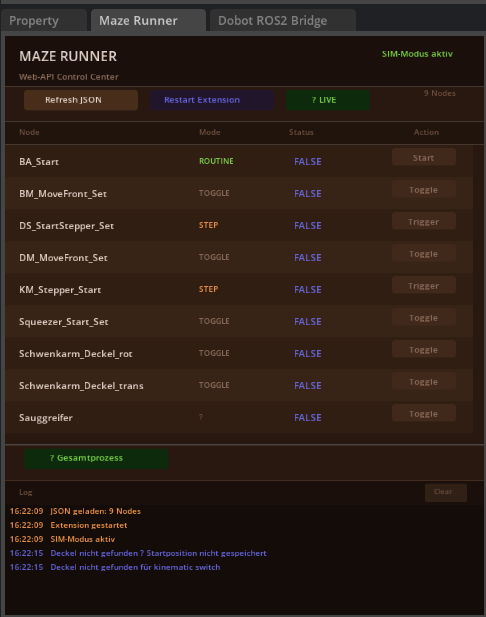
\includegraphics[height=10.4cm]{MazerunnerHMI}
        \caption{Maze-Runner-HMI.}
        \label{fig:mazerunner_hmi}
    \end{minipage}
    \hfill
    \begin{minipage}[t]{0.42\linewidth}
        \centering
        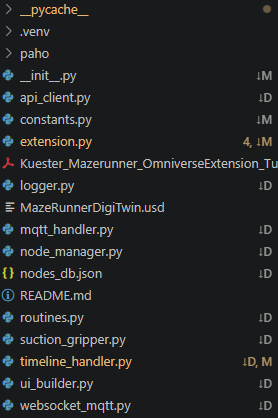
\includegraphics[height=10.4cm]{MazerunnerGithubRepo}
        \caption{Dateien des Extensionordners.}
        \label{fig:mazerunner_github_repo}
    \end{minipage}
\end{figure}

Aus Vollständigkeitsgründen wurde der Ordner um alle Dateien ergänzt, die für den Betrieb des Digitalen Zwillings notwendig sind, darunter eine Schritt-für-Schritt-Anleitung im PDF-Format (siehe Anhang~\ref{anhang:omniverse_tutorial}), die USD-Szene der Maze-Runner-Anlage, die bereits in Abbildung~\ref{fig:mazerunner_isaac} und Abbildung~\ref{fig:mazerunner_extension} zu sehen war, sowie eine \texttt{README.md}-Datei.
Dadurch lässt sich der Ordner später unverändert über ein GitHub-Repository bereitstellen, ohne dass weitere Dateien ergänzt werden müssen.
Der Ordner \texttt{\_\_pycache\_\_} enthält den von Python erzeugten Bytecode, der Ordner \texttt{.venv} die virtuelle Python-Umgebung mit allen Abhängigkeiten und der Ordner \texttt{paho} die externe MQTT-Bibliothek \texttt{paho-mqtt}.
Die Datei \texttt{\_\_init\_\_.py} kennzeichnet das Verzeichnis lediglich als Python-Paket.
Diese Bestandteile sind nicht spezifisch für die vorliegende Extension, weshalb im Folgenden nicht weiter auf sie eingegangen wird.
Der eigentliche Quellcode der Extension gliedert sich in die folgenden zwölf Module:

\begin{enumerate}
    \item \textbf{extension.py} -- Einstiegspunkt der Extension, implementiert die Klasse \texttt{MyExtension}, die von \texttt{omni.ext.IExt} erbt und damit vollständig in den Isaac-Sim-Lebenszyklus integriert ist, wobei die Methoden \texttt{on\_startup()} und \texttt{on\_shutdown()} Initialisierung und Ressourcenfreigabe aller asynchronen Tasks regeln und dabei alle Komponenten einrichten,
    \item \textbf{nodes\_db.json} -- Definiert über eine JSON-Konfigurationsdatei die Verknüpfung jedes SPS-Knotens mit dem Digitalen Zwilling, wobei jeder Eintrag die OPC-UA-Node-ID, den USD-Pfad des Zielgelenks, den Gelenktyp, den Zielwert sowie den Mode enthält, wie in Abbildung~\ref{fig:nodes_db} zu sehen ist.
    Das Feld \texttt{mode} legt dabei fest, wie ein Knoten auf einen Steuerbefehl reagiert.
    Für Bauteile, die nur zwischen zwei Endlagen wechseln, wie den Schieber, wird der Modus \emph{toggle} verwendet.
    Da sich Gelenke in Isaac Sim nur in eine im Feld \texttt{target\_value} hinterlegte Zielposition fahren lassen, ergibt sich für rotierende Bauteile wie die Drehscheibe die Schwierigkeit, eine fortlaufende Drehung abzubilden.
    Dafür wird der Modus \emph{impulse} genutzt, bei dem der bisherige \texttt{target\_value} um den im Feld \texttt{step\_degrees} hinterlegten Wert erhöht und als neuer \texttt{target\_value} gesetzt wird.
    Dieser Wert beträgt im vorliegenden Fall sechzig Grad, was der Anordnung der sechs vom induktiven Sensor detektierten Metallpins auf der Drehscheibe entspricht.
    Ein dritter Modus namens \emph{routine} führt eine Abfolge von mehreren Einzelaktionen durch, eine Schrittkette,
    \item \textbf{node\_manager.py} -- Lädt die Knoten aus \texttt{nodes\_db.json}, baut die Knotenliste im UI auf und fährt bei Zustandsänderungen die passenden Gelenke in der Szene über das Feld \texttt{target\_value} in ihre Zielposition,
    \item \textbf{ui\_builder.py} -- Baut das in NVIDIA Isaac Sim angedockte Maze-Runner-HMI einmalig auf und liefert Referenzen auf alle UI-Widgets an \texttt{extension.py} zurück, das gesamte in Abbildung~\ref{fig:mazerunner_hmi} gezeigte Fenster mit Statusanzeigen, Knotenlisten, Buttons, Überschriften, Logger und allen weiteren Komponenten,
    \item \textbf{api\_client.py} -- Sendet asynchrone HTTP-Requests an den \emph{DigitalTwinService} der Hochschule RheinMain und nutzt \texttt{node\_manager.py} zum Aktualisieren der Anzeige nach Antwort, wie in Abbildung~\ref{fig:blockdiagramm} über REST-API und MQTT-WebSocket dargestellt,
    \item \textbf{mqtt\_handler.py} -- Startet und stoppt den MQTT-WebSocket-Client und leitet eingehende Nachrichten thread-sicher in den asyncio-Loop weiter, wo \texttt{node\_manager.py} den Zustand aktualisiert,
    \item \textbf{websocket\_mqtt.py} -- Implementiert MQTT~v3.1.1 manuell über WebSocket und wird von \texttt{mqtt\_handler.py} genutzt, um Topics zu abonnieren und PUBLISH-Pakete zu empfangen,
    \item \textbf{deckel\_joint\_handler.py} -- Verwaltet die Startposition des Deckels, bildet den FixedJoint zwischen Sauggreifer und Deckel beim Aufnehmen und löst ihn beim Loslassen, erstellt anschließend den FixedJoint zwischen Deckel und Boden, aktualisiert die Deckelposition bei der Weiterbewegung des Bodens auf der Drehscheibe und senkt den Deckel beim Ausfahren der Presse ab,
    \item \textbf{routines.py} -- Enthält automatisierte Abläufe wie den Gesamtprozess und \texttt{BA\_Start}, die \texttt{node\_manager.py}, \texttt{deckel\_joint\_handler.py} und \texttt{extension.py} ansprechen,
    \item \textbf{timeline\_handler.py} -- Reagiert auf Play und Stop der Omniverse-Timeline, startet bei Play den SIM-Loop zum Halten und Verpressen des Deckels und setzt bei Stop alle Werte zurück,
    \item \textbf{logger.py} -- Schreibt Log-Zeilen direkt in das Fehlerausgabefenster und wird von allen Modulen genutzt, in Abbildung~\ref{fig:mazerunner_hmi} unten zu sehen, wobei die Zeilen je nach zugehörigem Modul in unterschiedlichen Farben dargestellt werden,
    \item \textbf{constants.py} -- Bündelt zentrale Konfigurationswerte wie API-Schlüssel, URLs, Farbwerte für Panelflächen und Geometrie-Offsets für die gesamte Extension.
\end{enumerate}

\begin{figure}[H]
    \centering
    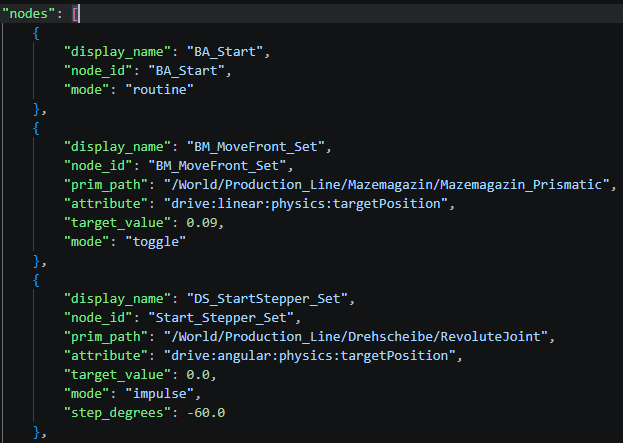
\includegraphics[width=0.85\linewidth]{nodes_db}
    \caption{Ausschnitt der Konfigurationsdatei \texttt{nodes\_db.json}.}
    \label{fig:nodes_db}
\end{figure}

\subsubsection{Maze-Runner-Netzwerkarchitektur}
\label{subsubsec:mazerunner_sps}

Von der Hochschule RheinMain (HSRM) wird gemeinsam mit Partnerhochschulen aus dem asiatischen und dem brasilianischen Raum eine Onlinevorlesung angeboten, in der alle beteiligten Hochschulen wechselseitig auf die Digitalen Zwillinge der anderen Standorte zugreifen können.
Diese hochschulübergreifende Vernetzung entspricht in der Hierarchieachse des RAMI-4.0-Modells der Ebene \emph{Vernetzte Welt}.
Die Maze-Runner-Anlage soll im Rahmen dieser Hochschulkooperation ebenfalls an die dafür genutzte Plattform, die \emph{Digital Twin App}, angebunden werden.
Das Ergebnis dieser Integration ist, dass sich die Anlage von überall steuern lässt und zudem das Bereitstellen eines Kamera-Livestreams der Anlage, das Live-Übertragen einer Isaac-Sim-Simulation sowie ein Panel mit Schaltflächen zur Fernsteuerung der Aktorik unterstützt werden, wie in Abbildung~\ref{fig:digitaltwinapp_dashboard} dargestellt ist.
Zudem ist die visuelle Programmiersprache \emph{Blockly} integriert, mit der sich einfache Anwendungen grafisch programmieren lassen.
Da all dies gebündelt in einer Oberfläche dargestellt werden kann, eignet sich die \emph{Digital Twin App} ideal für eine Onlinevorlesung mit Bildschirmübertragung.

\begin{figure}[H]
    \centering
    \fbox{\parbox[c][6cm][c]{0.8\linewidth}{\centering Platzhalter: Digital Twin App Dashboard}}
    \caption{Digital Twin App Dashboard.}
    \label{fig:digitaltwinapp_dashboard}
\end{figure}

Das Herzstück der Verbindung bildet der vom VPN-Router aufgebaute VPN-Tunnel zum Backend der \emph{Digital Twin App}, dem \emph{DigitalTwinService} der Hochschule RheinMain.
Der \emph{DigitalTwinService} kann darüber wiederum über den VPN-Tunnel die Anlage steuern, indem er die OPC-UA-Knoten der Maze-Runner-Anlage anspricht.

Die Gesamtarchitektur der Systemkommunikation ist in Abbildung~\ref{fig:blockdiagramm} dargestellt.
Sie umfasst drei Netzwerkzonen: das Netzwerk der Digitalen Fabrik im Labor, das Netzwerk der Hochschule RheinMain sowie das freie Internet.
Das Netzwerk der Digitalen Fabrik im Labor umfasst zusätzlich ein davon getrenntes Netzwerk der Maze-Runner-Anlage.
Das Netzwerk der Digitalen Fabrik ermöglicht der Maze-Runner-Anlage den Zugang zum Internet, was in Abbildung~\ref{fig:blockdiagramm} über den VPN-Tunnel dargestellt wird.
Der NVIDIA-Omniverse-Simulationsrechner befindet sich dabei im freien Internet und kommuniziert ortsungebunden per REST API mit dem \emph{DigitalTwinService}.
Auch die Website \emph{DigitaltwinApp.de} ist aus dem freien Internet erreichbar.

\begin{figure}[H]
    \centering
    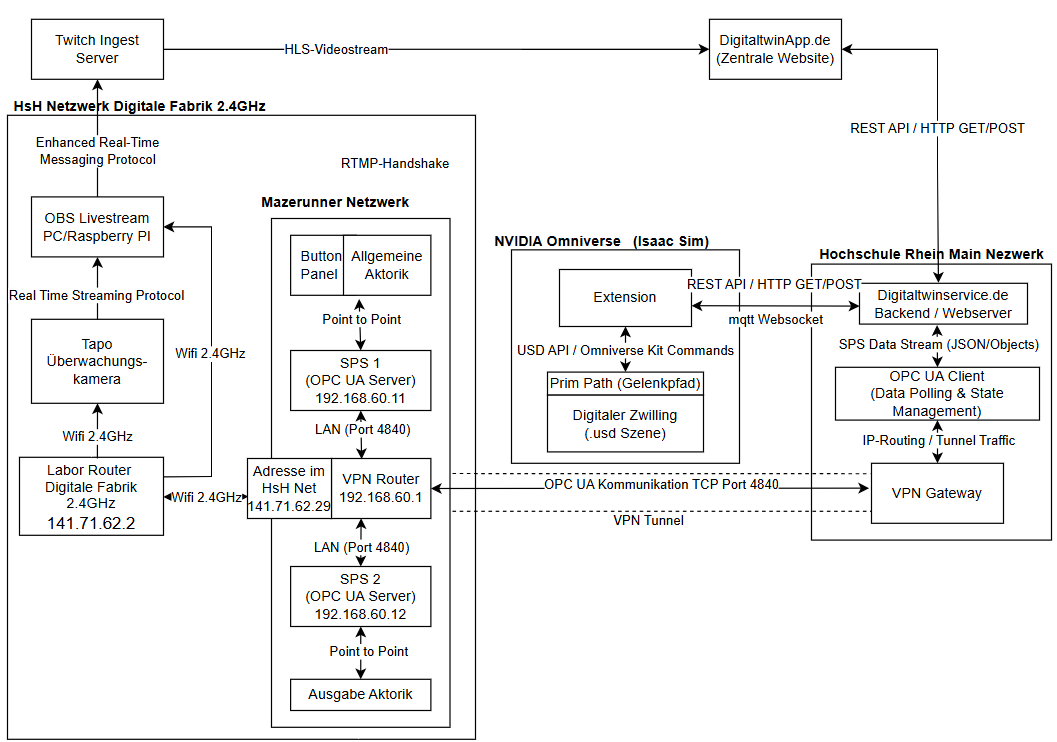
\includegraphics[width=\linewidth]{Internal_Block_Diagram}
    \caption{Netzwerkarchitektur zur Anbindung Digitaler Zwillinge in NVIDIA Omniverse an die Digital Twin App der Hochschule RheinMain (HSRM).}
    \label{fig:blockdiagramm}
\end{figure}

Ein Steuersignal wird dabei von der Extension per REST-API an den \emph{DigitalTwinService} übermittelt, der es als SPS-Datenstrom an den OPC-UA-Client der Hochschule RheinMain weiterleitet.
Von dort gelangt das Signal über das VPN-Gateway und den VPN-Tunnel zum VPN-Router im Netzwerk der Maze-Runner-Anlage, der es über die SPS an die Aktorik weiterleitet.
Der VPN-Router lässt sich dabei per VPN-Tunnel vom Netzwerk der Hochschule RheinMain aus erreichen, wobei der Labor-Router Digitale Fabrik die Verbindung zum Internet bereitstellt.

Der Kamera-Livestream nimmt dagegen einen eigenen Weg.
Die Tapo-Überwachungskamera überträgt ihr Bild per RTSP an einen OBS-Livestream-Rechner, welcher in diesem Fall der Laptop ist, auf dem auch die NVIDIA-Isaac-Sim-Instanz ausgeführt wird.
Dieser leitet das Bild per RTMP an einen Twitch-Ingest-Server weiter, von dem aus die \emph{Digital Twin App} den Stream als HLS-Videostream einbindet.
Die Überwachungskamera erhält ihre Internetverbindung ebenfalls über den Laborrouter Digitale Fabrik.
Dabei wird lediglich das Bild der Kamera übertragen, eine Fernsteuerung der Gier- und Nickmotorik der Überwachungskamera wird nicht unterstützt.

Die bidirektionale Datenkopplung zwischen Extension und \emph{DigitalTwinService} wird über zwei Protokolle realisiert.
Zum Fernsteuern der Anlage wird die REST-API genutzt, über die Steuerbefehle als HTTP-POST mit Authentifizierung übermittelt werden, woraufhin der \emph{DigitalTwinService} den OPC-UA-Schreibzugriff auf die SPS über einen verschlüsselten VPN-Tunnel ausführt.
Da die REST-API jedoch nicht über eine Publish-Subscribe-Architektur verfügt und eine Wertänderung sonst durch wiederholtes, ressourcenintensives Abfragen erkannt werden müsste, wird zum Empfangen geänderter Anlagenwerte stattdessen die MQTT-WebSocket-Schnittstelle des \emph{DigitalTwinService}-Backends genutzt, über die die Extension ressourcenarm auf Wertänderungen lauschen kann.
Der vollständige Steuerpfad lautet: Isaac-Sim-Extension $\rightarrow$ REST-HTTP $\rightarrow$ DigitalTwinService $\rightarrow$ OPC-UA-WriteValue $\rightarrow$ SPS.
Die typische Latenz dieses Steuerpfades liegt zwischen \SI{100}{\milli\second} und \SI{500}{\milli\second}.

\subsubsection{Inbetriebnahme und Optimierung}
\label{subsubsec:mazerunner_inbetriebnahme}

Bei der Übergabe der Anlage von Herrn Wang an das LFP befand sich diese im in Abbildung~\ref{fig:ist_zustand_mazerunner} gezeigten Ist-Zustand.
Im Vergleich zum finalen Tischaufbau aus Abbildung~\ref{fig:dobot_mazerunner_tisch} waren daher zahlreiche Schritte zur Inbetriebnahme und Optimierung der Anlage notwendig, die gemeinsam mit Herrn Wang festgelegt wurden.

\begin{figure}[H]
    \centering
    \makebox[\linewidth][c]{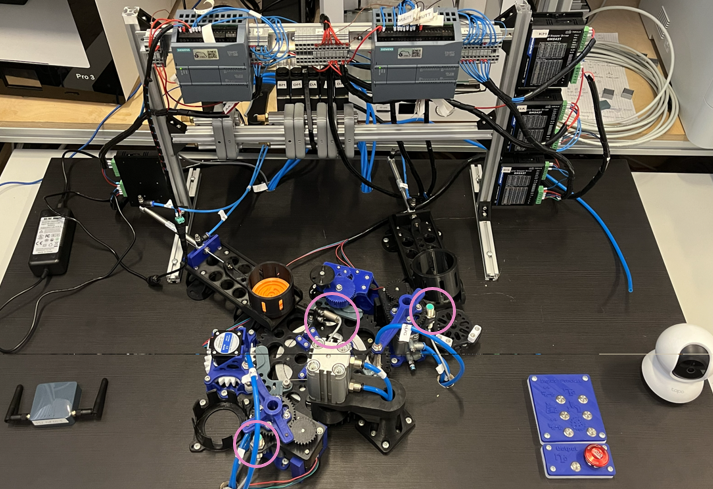
\includegraphics[width=1.25\linewidth]{Ist-Zustand_Mazerunner}}
    \caption{IST-Zustand der Maze-Runner-Anlage im Hochschullabor (Aufnahme von oben).}
    \label{fig:ist_zustand_mazerunner}
\end{figure}

Im Rahmen der Inbetriebnahme wurden Anpassungen an Halterungen, Elektrik, SPS und Druckluftversorgung vorgenommen, auf die im Folgenden genauer eingegangen wird.

Für den Betrieb mit dem Arbeitsdruck von vier Bar musste ein Druckluftminderer mit den passenden Anschlüssen verbaut werden, der eingangsseitig mit der Schnellkupplung verbunden ist und ausgangsseitig über den sechs Millimeter durchmessenden Schlauch die Magnetventile speist.

Die Inbetriebnahme begann mit dem VPN-Router, der zunächst in das Netzwerk der Digitalen Fabrik im Labor aufgenommen und freigegeben werden musste, damit er die Hochschule RheinMain und darüber den \emph{DigitalTwinService} erreichen kann.
Anschließend musste sichergestellt werden, dass die SPS im selben Subnetz wie der Router konfiguriert ist, sodass beide SPS-Anlagen über den Router im selben Netz erreichbar sind.
Ergänzend wurde die Kamera in Betrieb genommen und mit einem eigenen Stativ ausgestattet.

Im elektrischen Bereich wurde eine Kaltgerätebuchse mit integriertem Schalter verbaut, über den sich die gesamte Anlage spannungsfrei schalten lässt.
Die aus der Schuko-Steckdose gespeisten 230\,V werden dabei über diesen Schalter auf die Eingänge des neuen WAGO-Netzteils geschaltet, welches die gesamte Anlage anschließend mit 24\,V Gleichspannung versorgt.
Dabei wurde außerdem der zunächst nicht angeschlossene Not-Aus-Schalter ergänzt, welcher die Versorgungsspannung der Aktorik separat von der SPS-Versorgungsspannung spannungsfrei schaltet, wodurch die SPS im Not-Aus-Fall nicht vollständig spannungsfrei geschaltet wird.
Hierfür mussten weitere Kabel verlängert, ergänzt oder ausgetauscht werden, was durch einen Ende-zu-Ende-Schaltplan in der Dokumentation unterstützt wurde.
Das neue WAGO-Netzteil ist zudem leistungsfähiger als das zuvor in Abbildung~\ref{fig:ist_zustand_mazerunner} sichtbare Netzteil und glättet Spannungsspitzen im HsH-Netz, wodurch die SPS vor Beschädigung geschützt wird.
Zudem wurde das Kabelmanagement optimiert, etwa durch den Verbau von Kabelkanälen auf der Rückseite der Aluminiumprofile sowie das Bündeln von Kabeln und Schläuchen mittels Klettkabelbindern.
Der VPN-Router wird dabei über einen eigenen DC-DC-Wandler von 24\,V auf 5\,V versorgt.

An der SPS selbst waren die Konfiguration in TIA Portal, insbesondere die Änderung der IP-Adresse, sowie der Erwerb der notwendigen Lizenzen für TIA Portal und das zugehörige Safety-Paket aufwendig.

Während der Inbetriebnahme wurden sämtliche Halterungen ergänzt und optimiert.
Die graue Halterung der Magnetventile wurde entfernt, diese wurden stattdessen direkt am Aluminiumprofil verschraubt.
Die treppenförmige Halterung der Schrittmotortreiber wurde von der Hochschule RheinMain (HSRM) entwickelt.
Im Rahmen dieser Arbeit wurde sie um eine weitere Stufe erweitert und ermöglicht eine zugängliche und kompakte Montage.
Die Halterung des induktiven Sensors, der die Drehscheibenbewegung erfasst, war gebrochen und musste neu ausgedruckt werden.
Der VPN-Router erhielt ebenfalls eine eigene Halterung, die zugleich den zugehörigen DC-DC-Wandler beherbergt.
Bei den meisten Halterungen mussten nachträglich Bohrungen in Autodesk Inventor hinzugefügt werden, damit sie mit dem Aufbau verschraubt werden konnten.
Auch die Bodenplatten der Magazin- und Deckelrutsche sowie deren Schieber mussten aufgrund der potenziellen Verkeilung in den vorhandenen Bohrungen angepasst werden.
Die Schieber wurden dabei zugleich neu skaliert.

Zuletzt mussten alle Stationen sowie die drei induktiven Sensoren genauestens justiert werden, da der Produktionsfluss nur funktioniert, wenn es millimetergenau abgestimmt ist.

Im Rahmen der Inbetriebnahme mussten zudem einzelne Bauteile neu beschafft werden.
Für das Kugelmagazin wurden Metallkugeln mit einem Durchmesser von drei Millimetern bestellt.
Der fehlende Saugnapf der Ausgabeschwenkarmstation wurde nachbestellt.

Im speziellen Aufbau der HsH ist zunächst nur ein einzelner Fertigungszyklus vorgesehen, weshalb das Magazin vorerst weggelassen wird.

Neben den offensichtlichen inbetriebnahmerelevanten Anpassungen stellte Herr Wang auch Anforderungen zur Weiterentwicklung der Anlage, die er während der Optimierungsphase im zweiwöchigen Rhythmus über Microsoft Teams besprach und in Jira festhielt.
Das in Abbildung~\ref{fig:kanban} gezeigte Kanban-Board gliedert die Aufgaben in die Spalten \emph{To Do}, \emph{In Progress} und \emph{Done} und enthält unter anderem die bereits umgesetzte Halterung für die Schrittmotortreiber, den Not-Aus sowie die Flexibilisierungsschablone mit Dobot-Einsatz.
Als in Bearbeitung befindlicher Punkt ist zudem der Ersatz des induktiven Sensors durch einen mechanischen Endlagenschalter aus Kostengründen vermerkt.
Dieser Ersatz wurde bereits erprobt, erreichte jedoch nicht die notwendige Zuverlässigkeit.
Als offener Punkt ist außerdem eine Motion Control für Level 3 vermerkt, bei der anhand des Signals eines Endlagenschalters und der Schrittzahl des Schrittmotors die genaue Position des Schwenkarms bestimmt werden soll.

\begin{figure}[H]
    \centering
    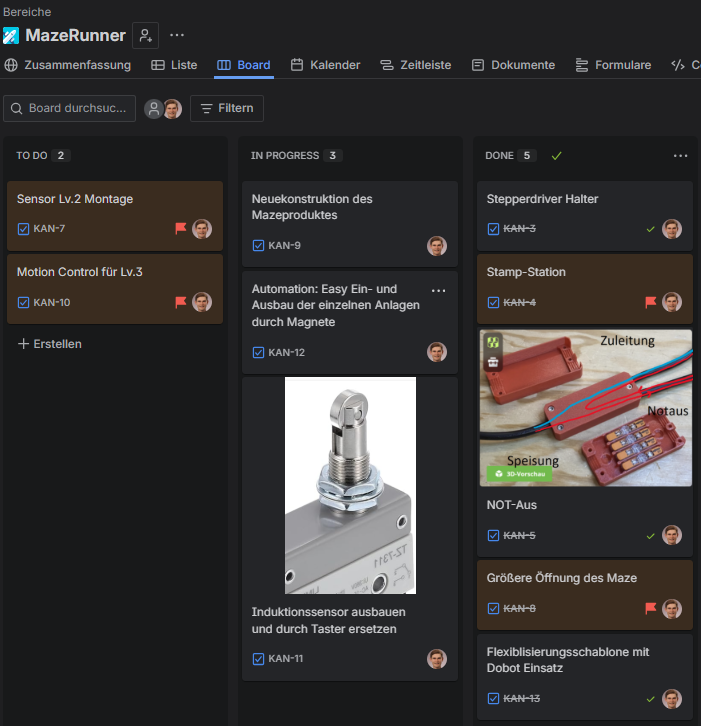
\includegraphics[width=0.9\linewidth]{Jira.png}
    \caption{Task-Tracking-Tool Jira von Atlassian, Maze-Runner-Weiterentwicklung (Stand: Juni 2026)}
    \label{fig:kanban}
\end{figure}

Durch die beschriebenen Schritte wurde die Produktion eines Mazeprodukts mit dem Rundtakttisch Maze-Runner zuverlässig realisiert.
Im speziellen Aufbau der Maze-Runner-Anlage an der HsH wurde dabei zunächst kein Wert auf die Zuführung weiterer Bauteile gelegt, da die Entwicklung des Digitalen Zwillings im Vordergrund stehen soll.

% -----------------------------------------------------------------------
\subsection{Anlage 2: Desktoproboter \enquote{Dobot Magician}, Pick-and-Place-Szenario}

In der produzierenden Industrie bilden Pick-and-Place-Aufgaben (PnP) einen fundamentalen Bestandteil jeder automatisierten Fertigungslinie und werden neben Magnet- und Zangengreifern auch über Vakuumsauggreifer realisiert, welche besonders flexibel einsetzbar sind.
Dabei werden Werkstücke automatisiert gegriffen, transportiert und abgelegt, was die Grundlage für Montage-, Sortier- und Palettieraufgaben quer durch alle Branchen bildet.
Der Ablauf gliedert sich in der Regel in die Schritte Anfahren, Greifen, Verfahren, Ablegen und Rückfahren.
Im Rahmen dieser Arbeit wird daher ein Pick-and-Place-Szenario als Anwendungsfall für den Dobot~Magician definiert, bei dem die anzufahrenden Punkte per Teach-In-Methode an den Dobot übergeben und später automatisiert abgefahren werden.
Konkret wird dabei zunächst die auf dem als Würfel mit vier Zentimetern Kantenlänge abstrahierten FTS abgelegte Schutzkappe angesaugt und anschließend auf das Heck eines Modellfahrzeugs des DeLorean aus \enquote{Zurück in die Zukunft} montiert, wie in Abbildung~\ref{fig:dobot_pp_szenario} zu sehen ist.

\begin{figure}[H]
    \centering
    \begin{minipage}[t]{0.42\linewidth}
        \centering
        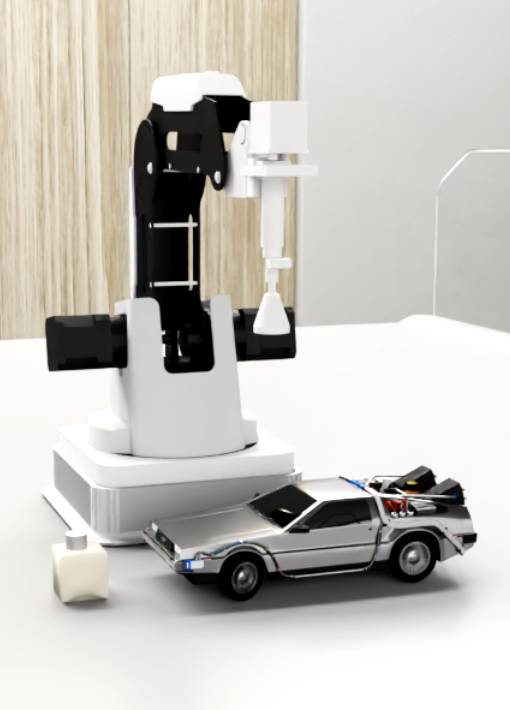
\includegraphics[width=\linewidth]{Dobot_PP_Scenario_mitte}
        \caption{Aufbau des PnP-Szenarios in NVIDIA Isaac Sim.}
        \label{fig:dobot_pp_szenario}
    \end{minipage}
    \hfill
    \begin{minipage}[t]{0.50\linewidth}
        \centering
        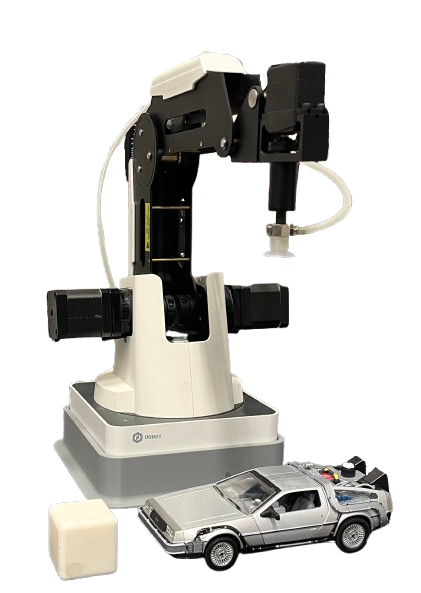
\includegraphics[width=0.85\linewidth]{DobotPnPLfp}
        \caption{Aufbau des PnP-Szenarios im LFP.}
        \label{fig:dobot_labor}
    \end{minipage}
\end{figure}

\subsubsection{Beschreibung der Anlage}
Der Dobot Magician ist ein vierachsiger Desktop-Roboterarm (Dobot Robotics Co.,~Ltd., Shenzhen, China), der für den Einsatz in der universitären Lehre konzipiert wurde~\cite{dobot_magician}.
Er realisiert eine Kinematik mit vier Freiheitsgraden (Degrees of Freedom, DOF) und den Gelenken J1 (Basisrotation), J2 (Schulter), J3 (Ellbogen) und J4 (Werkzeugkopf) bei einer maximalen Reichweite von \SI{320}{\milli\meter} und einer Nutzlast von bis zu \SI{500}{\gram}.
Die Kommunikation mit dem Rechner erfolgt über USB mittels eines proprietären seriellen Protokolls.

\begin{figure}[H]
    \centering
    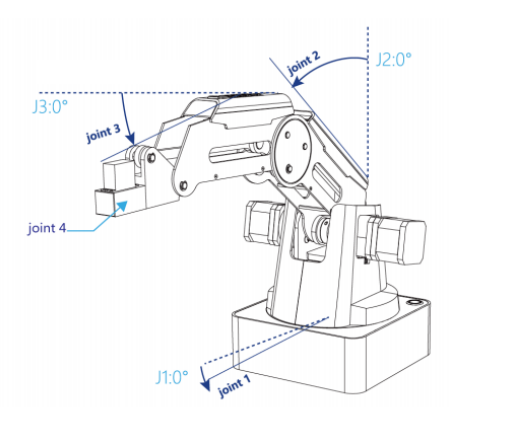
\includegraphics[width=0.55\linewidth]{Dobot_Gelenkwinkel}
    \caption{Gelenkwinkelkonvention des Dobot Magician mit den Nullstellungen der Gelenke J1 bis J4 (Quelle: \cite{kuester2026dobottutorial}).}
    \label{fig:dobot_gelenkwinkel}
\end{figure}

Der Dobot Magician besitzt ein Parallelogrammgetriebe im Unterarm, das die Werkzeugplatte unabhängig von Schulter- und Ellbogengelenk horizontal ausrichtet.
Dadurch können mit dem Sauggreifer ausschließlich Bauteile von oben gegriffen werden, wobei sich dessen Orientierung nur durch eine Drehung um die Z-Achse verändern lässt.
Dieses Getriebe bildet eine geschlossene kinematische Kette, die für die Simulation besondere Anforderungen stellt (vgl.\ Abschnitt~\ref{subsubsec:dobot_urdf}).

Als Endeffektor für das Pick-and-Place-Szenario ist am Dobot Magician ein pneumatischer Sauggreifer montiert.
Dieser besteht aus einem Saugkopf mit Luftschlauchanschluss am vierten Gelenk sowie einer separaten Pumpeneinheit, die über die digitalen Anschlüsse GP1, GP3 und SW1 angesteuert wird, wie Abbildung~\ref{fig:dobot_sauggreifer} zeigt~\cite{kuester2026dobottutorial}.
In dieser Abbildung ist zudem Joint~4 zu sehen, der als Servomotor den unteren Teil des Endeffektors dreht.
Die Pumpe wird über GP1 und SW1 mit der Steuerung des Dobot Magician verbunden, während der Saugkopf über GP3 am vierten Gelenk angeschlossen wird, wie Abbildung~\ref{fig:dobot_sauggreifer_anschluss} zeigt~\cite{kuester2026dobottutorial}.

\begin{figure}[H]
    \centering
    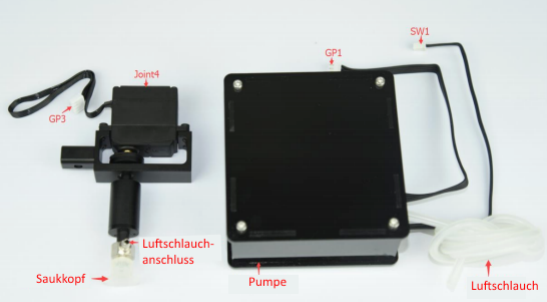
\includegraphics[width=0.7\linewidth]{Sauggreifer}
    \caption{Komponenten des pneumatischen Sauggreifers, Saugkopf mit Luftschlauchanschluss (links) und Pumpeneinheit mit den Anschlüssen GP1 und SW1 (rechts) (Quelle: \cite{kuester2026dobottutorial}).}
    \label{fig:dobot_sauggreifer}
\end{figure}

\begin{figure}[H]
    \centering
    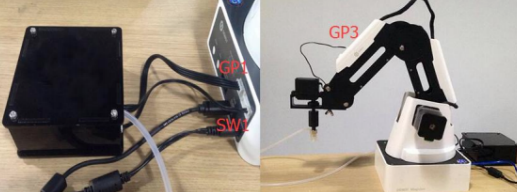
\includegraphics[width=0.6\linewidth]{Sauggreifer_Anschließen}
    \caption{Anschluss des Sauggreifers, Verkabelung der Pumpe über GP1 und SW1 (links) sowie Anbindung des Saugkopfs über GP3 am vierten Gelenk (rechts) (Quelle: \cite{kuester2026dobottutorial}).}
    \label{fig:dobot_sauggreifer_anschluss}
\end{figure}

Die gezeigte Hardware soll nun in NVIDIA Isaac Sim zu einem Digitalen Zwilling überführt werden, wofür eine NVIDIA-Isaac-Sim-Extension entwickelt wird, die das Pick-and-Place-Szenario realisiert.

\subsubsection{Problemstellung und Konzept für den Digitalen Zwilling}
\label{subsubsec:dobot_konzept}
Der Dobot Magician weist gegenüber dem Maze-Runner grundlegend andere Randbedingungen auf, die eine eigenständige Konzeption des Digitalen Zwillings erfordern.
Während die SPS-gestützte Anlage über standardisierte Schnittstellen und ein etabliertes OPC-UA-Informationsmodell verfügt, kommuniziert der Dobot Magician ausschließlich über ein proprietäres, seriell-basiertes USB-Protokoll.
Dieses Protokoll ist nicht nativ in ROS\,2 oder Isaac Sim integriert, was eine Middleware-Schicht notwendig macht.
Zudem ist eine direkte bidirektionale Steuerung aus der Simulation heraus aufgrund fehlender Echtzeitrückkopplung auf Gelenkebene in der Anfangsausbaustufe nicht vorgesehen.
Das Ziel ist zunächst die Realisierung eines Digitalen Schattens nach Kritzinger et al., der die Gelenkzustände des physischen Roboters kontinuierlich im virtuellen Modell abbildet~\cite{kritzinger2018}.

Das Konzept sieht eine zweistufige Architektur vor.
In der ersten Stufe liest ein direkt unter Windows ausgeführtes, auf der \emph{pydobot}-Bibliothek basierendes Python-Skript die Gelenkwinkel J1--J4 zyklisch aus und publiziert diese als standardisierte \texttt{sensor\_msgs/JointState}-Nachrichten, wofür die intern vorinstallierte ROS\,2-Extension von NVIDIA Isaac Sim die Middleware bildet.
In der zweiten Stufe empfängt Isaac Sim diese Nachrichten über einen \emph{ROS\,2~Subscribe-JointState}-Knoten im Action~Graph und überträgt die Winkelwerte auf die importierte USD-Articulation des Roboters.
Die kinematische Grundlage bildet eine URDF-Beschreibung, die aus den CAD-Daten des Herstellers abgeleitet und mit Gelenklimits sowie Achsparametern versehen wird.

Dieses Konzept ist ohne proprietäre Lizenzkosten realisierbar und erlaubt eine vollständige Entwicklung und Erprobung ohne physische Hardware durch den Einsatz eines Software-Mocks für die Gelenkkommunikation.

\subsubsection{URDF-Modellierung und Import in NVIDIA Isaac Sim}
\label{subsubsec:dobot_urdf}

\begin{figure}[H]
    \centering
    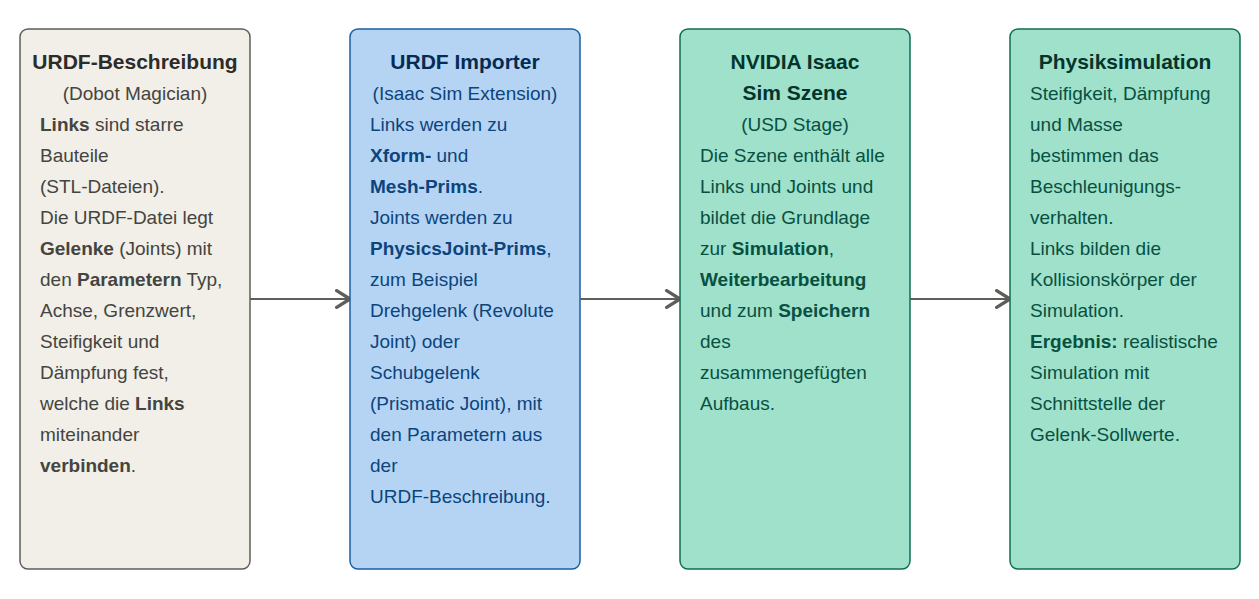
\includegraphics[width=\linewidth]{aufbau_digitaler_zwilling_urdf_usd_horizontal}
    \caption{Aufbau des Digitalen Zwillings von der URDF-Beschreibung zur NVIDIA Isaac Sim Szene.}
    \label{fig:dobot_urdf_aufbau}
\end{figure}

Wie in Abbildung~\ref{fig:dobot_urdf_aufbau} zu sehen ist, wird die kinematische Struktur des Dobot Magician in einer URDF-Datei formalisiert.
Die vier Glieder werden als STL-Meshes referenziert. Die zugehörigen Gelenke erhalten Drehachsen, Bewegungsgrenzen und Antriebsparameter~\cite{ros_urdf}.
Die Roboterbasis wird über einen starren Weltanker verankert, um physikalische Stabilität zu gewährleisten.
Der Isaac-Sim-URDF-Importer überführt die Beschreibung in eine USD-Articulation. Die Optionen \emph{Merge Fixed Joints} und \emph{Fix Base Link} müssen dabei aktiviert sein.
Die Eigenschaft \emph{Instanceable} ist für alle beweglichen Gelenke zu deaktivieren, da der Action~Graph sonst keine Schreibzugriffe auf die Gelenktransformationen erhält~\cite{nvidia_isaacsim}.

Eine Herausforderung stellt das Parallelogrammgetriebe des Unterarms dar.
Dieses bildet eine geschlossene kinematische Kette: Zwei mechanische Pfade zwischen Schultergelenk und Werkzeugplatte erzeugen gegenseitige Abhängigkeiten, die über einfache Vorwärtskinematik nicht auflösbar sind.
Physik-Engines wie NVIDIA PhysX unterstützen ausschließlich offene kinematische Bäume. Geschlossene Schleifen erfordern entweder explizite Schleifenschlussbedingungen oder eine vereinfachte Modellierung~\cite{nvidia_physx}.
Im vorliegenden Modell wird die geschlossene Kette durch eine Näherung als offene Kette abgebildet. Das Parallelogrammgetriebe wird im URDF nicht vollständig modelliert, stattdessen wird die Parallelführung durch die Gelenkkonfiguration angenähert.
Für den angestrebten Digitalen Schatten ist diese Vereinfachung hinreichend, da die Darstellung der Endeffektorpose im Vordergrund steht, nicht die exakte Simulation der internen Mechanik.

\subsubsection{Systemarchitektur und ROS\texorpdfstring{\,}{}2-Anbindung}
Die Datenkopplung zwischen realem Roboter und NVIDIA Isaac Sim wird vollständig lokal ohne externe Netzwerkabhängigkeiten realisiert.
Die Hardware-Anbindung erfolgt über ein direkt unter Windows ausgeführtes Python-Bridge-Skript, das über die \emph{pydobot}-Bibliothek die aktuellen Gelenkwinkel J1--J4 direkt aus dem Roboter ausliest.

Ein wesentlicher Unterschied zum Maze-Runner besteht in der Art der übertragenen Signale.
Die Siemens-SPS verarbeitet diskrete Schaltsignale, während die pydobot-Schnittstelle kontinuierliche Gelenkwinkel in Grad zurückliefert.
Das Bridge-Skript rechnet diese Werte in Bogenmaß um und publiziert sie mit \SI{20}{\hertz} als \texttt{sensor\_msgs/JointState}-Nachricht im lokalen ROS\,2-Netz, wofür die intern vorinstallierte ROS\,2-Extension von NVIDIA Isaac Sim die Middleware bildet.

Die Aktuierung in NVIDIA Isaac Sim erfolgt über den Action~Graph.
Ein \emph{ROS\,2~Subscribe-JointState}-Node empfängt die Winkelwerte und leitet sie über einen \emph{Articulation~Controller} an die URDF-Gelenkhierarchie weiter.
Damit ist eine funktionale Synchronisation im Sinne eines Digitalen Schattens nach Kritzinger et al.\ realisiert~\cite{kritzinger2018}.
Eine weitergehende Validierung und der Ausbau zur bidirektionalen Steuerung sind Gegenstand zukünftiger Arbeiten.

\subsubsection{Inbetriebnahme}
\label{subsubsec:dobot_inbetriebnahme}

Die Inbetriebnahme des Dobot-Magician-Digitalen-Zwillings erfolgte in drei aufeinanderfolgenden Phasen.

In der ersten Phase wurden die Systemvoraussetzungen geschaffen.
Auf dem Windows-Host wurden ROS\,2~Humble sowie die \emph{pydobot}-Bibliothek installiert.

In der zweiten Phase wurde die Datenkommunikation validiert.
Das Bridge-Skript wurde mit dem physischen Roboter verbunden und die ausgelesenen Gelenkwinkel J1--J4 auf Plausibilität geprüft.
Die ROS\,2-Topics wurden auf korrekte \texttt{sensor\_msgs/JointState}-Nachrichten im 20-Hz-Takt überprüft.
Für die hardware-unabhängige Entwicklung wurde ein Software-Mock eingesetzt, der die vollständige Pipeline ohne physischen Roboter testbar macht.

In der dritten Phase wurde die Isaac-Sim-Anbindung konfiguriert.
Der URDF-Import wurde mit den dokumentierten Parametern durchgeführt und der Action~Graph mit dem \emph{ROS\,2~Subscribe-JointState}-Knoten verbunden.
Die Bewegungsübertragung wurde visuell durch parallele Beobachtung von physischem Roboter und virtuellem Modell verifiziert.
Da in der Anfangsausbaustufe keine Echtzeitregelung vorgesehen ist, entfällt eine Optimierungsschleife.
Der Fokus liegt auf der stabilen Übertragung der Gelenkzustände als Digitaler Schatten nach Kritzinger et al.~\cite{kritzinger2018}.

\section{Dokumentation der Entwicklungspipeline}
\label{sec:ergebnisse}

Damit die entwickelten Digitalen Zwillinge über die Laufzeit dieser Arbeit hinaus im LFP genutzt, gewartet und auf weitere Anlagen übertragen werden können, mussten Entwicklungsergebnisse, Reproduktionsschritte und Übergabeartefakte durchgängig dokumentiert werden. Dieses Kapitel fasst zunächst die beiden entstandenen Softwareerweiterungen zusammen, beschreibt anschließend die Reproduzierbarkeitsdokumentation und schließt mit einer Gegenüberstellung beider Anlagen.

\subsection{Omniverse-Extension und ROS\,2-Anbindung als Entwicklungsergebnisse}

Im Rahmen dieser Arbeit wurden zwei funktionsfähige Softwareerweiterungen für NVIDIA Isaac Sim entwickelt, erprobt und an das LFP übergeben.

\textbf{Maze-Runner-Extension:} Die entwickelte modulare Extension im \emph{Omniverse Kit Extension Framework} gliedert sich in zwölf spezialisierte Module (vgl.\ Abschnitt~\ref{subsubsec:mazerunner_extension}) und koppelt die Siemens-SPS S7-1200 über den \emph{DigitalTwinService} bidirektional an den Digitalen Zwilling in NVIDIA Isaac Sim. Die datengetriebene Konfiguration über \texttt{nodes\_db.json} ermöglicht die Übertragung der Extension auf weitere SPS-gestützte Anlagen ohne Quellcodeänderungen. Der Steuerpfad von der Extension zur SPS erreicht dabei eine Latenz zwischen \SI{100}{\milli\second} und \SI{500}{\milli\second} (vgl.\ Abschnitt~\ref{subsubsec:mazerunner_sps}). Die Rückmeldung der Sensorwerte aus der SPS an den Digitalen Zwilling über die MQTT-WebSocket-Schnittstelle ließ sich im Laborbetrieb dagegen nicht durchgängig zuverlässig nachweisen, worauf Abschnitt~\ref{subsec:gesamtbewertung} genauer eingeht.

\textbf{Dobot-Magician-Extension:} Für den Dobot Magician entstand mit \texttt{Dobot\_DT\_IsaacSim\_Extension} eine eigenständige Kit-Extension, deren Klasse \texttt{DobotROSNode} über die \emph{pydobot}-Bibliothek zyklisch die Pose des realen Roboters ausliest und die berechneten Gelenkwinkel direkt über die in Isaac Sim integrierte Dynamic-Control-API auf die Articulation des importierten Robotermodells schreibt. In Gegenrichtung sendet die Extension über ein Bedienpanel Jog-Befehle, Vakuumgreifer-Schaltungen sowie automatisierte Pick-and-Place-Sequenzen an den realen Gelenkarmroboter, wobei Letztere zuvor per Teach-In am physischen Gelenkarmroboter aufgezeichnet wurden. Beide Erweiterungen sind im GitHub-Repository versioniert und gemäß der Reproduzierbarkeitsdokumentation (vgl.\ Abschnitt~\ref{subsec:reprodoku}) nachvollziehbar.

\subsection{Reproduzierbarkeitsdokumentation}
\label{subsec:reprodoku}

Damit beide Digitalen Zwillinge unabhängig von den beteiligten Personen reproduziert werden können, wurde für jede Anlage eine eigenständige Anleitung erstellt und in komplementären Medienformaten an das LFP übergeben.

\subsubsection{Methodische Schritt-für-Schritt-Anleitung -- Maze Runner}
Aus den Erfahrungen der Modellerstellung wurde eine generische Anleitung in sieben Schritten abgeleitet (vgl.\ Anhang~\ref{anhang:repro}):
\begin{enumerate}
    \item Anforderungsanalyse und Schnittstellenmatrix der Zielanlage,
    \item CAD-Aufbereitung und Export nach OpenUSD,
    \item Definition kinematischer Strukturen in NVIDIA Isaac Sim (Articulations),
    \item Auswahl und Einrichtung der geeigneten Middleware (OPC~UA, MQTT, ROS\,2),
    \item Implementierung der bidirektionalen Datenkopplung,
    \item Validierung anhand definierter Testszenarien,
    \item Übergabe und Versionierung im GitHub-Repository.
\end{enumerate}

\subsubsection{Reproduzierbarkeitsdokumentation Dobot Magician}
Analog zur Maze-Runner-Dokumentation wurde für den Dobot Magician eine eigenständige Inbetriebnahme-Anleitung erstellt. Diese umfasst:
\begin{enumerate}
    \item Einrichtung von \emph{pydobot} unter Windows sowie Installation der Extension \texttt{Dobot\_DT\_IsaacSim\_Extension} über den Extension-Manager oder das Hilfsskript \texttt{install\_extension.py},
    \item URDF-Import in NVIDIA Isaac Sim mit den erforderlichen Parametereinstellungen (\emph{Merge Fixed Joints}, \emph{Fix Base Link}, deaktiviertes \emph{Instanceable}),
    \item Verifikation der Dynamic-Control-Kopplung anhand der Gelenkzustandsübertragung,
    \item Betrieb des Software-Mocks für hardware-unabhängige Entwicklung und Tests.
\end{enumerate}
Alle Schritte sind im GitHub-Repository versioniert. Die Anleitung ist so strukturiert, dass sie ohne physischen Roboter vollständig nachvollzogen werden kann.

\subsubsection{Medienformate}
Die Anleitungen wurden in komplementären Formaten aufbereitet:
\begin{enumerate}
    \item \textbf{Foliensatz} (PowerPoint, 32 Folien) als didaktische Grundlage für Lehrveranstaltungen,
    \item \textbf{VR-Demonstration} auf Meta Quest~3 zur immersiven Inspektion der Digitalen Zwillinge,
    \item \textbf{Maze-Runner-GitHub-Repository} mit allen im Rahmen dieser Arbeit erarbeiteten Dateien, von der Installation von NVIDIA Isaac Sim über die Konfiguration der SPS und die Anbindung an die Netzwerkinfrastruktur der Hochschule RheinMain bis hin zur Extension selbst mit ihren Modulen sowie der Maze-Runner-USD-Szene,
    \item \textbf{Dobot-Extension-GitHub-Repository} mit der technischen Dokumentation der Dobot-Magician-Extension, der URDF-Datei mit den zugehörigen CAD-Dateien sowie Hilfsskripten, etwa zur Kalibrierung, zur Installation der Extension oder zum Setzen des Extension-Pfads unter Windows.
\end{enumerate}
Beide Anleitungen wurden von mehreren Personen getestet, deren Rückmeldungen eingearbeitet wurden.

\subsubsection{Übergabe an das LFP}
Alle erstellten Artefakte -- USD-Stages, URDF-Dateien, Python-Extensions, OPC-UA-Konfigurationen, Reproduktionsanleitungen und die schriftliche Ausarbeitung -- wurden gemäß Aufgabenstellung digital an das LFP übergeben und in einem GitHub-Repository versioniert. Eine Veröffentlichung innerhalb der für IEEE geplanten Schriftenreihe des LFP ist vorgesehen.

\subsection{Gegenüberstellung und Gesamtbewertung}
\label{subsec:gesamtbewertung}

Beide Anlagen bestätigen die Machbarkeit einer durchgängigen Datenkette von CAD über OpenUSD bis zur Echtzeit-Simulation in NVIDIA Isaac Sim ohne proprietäre Konvertierungsschritte~\cite{pixar_openusd}. Die Protokollwahl, OPC~UA und MQTT für die SPS-Anlage sowie ROS\,2 für den Roboter, richtet sich nach den unterschiedlichen Kommunikationsanforderungen beider Anlagen.

Beim Maze Runner ließ sich die Rückmeldung der Sensorwerte aus der SPS an den Digitalen Zwilling über die MQTT-WebSocket-Schnittstelle im Laborbetrieb nicht durchgängig echtzeitfähig nachweisen. Über den eingerichteten Subscribe-Mechanismus gingen zwar MQTT-Pakete ein, jedoch nicht durchgängig echtzeitfähig und zuverlässig genug, um als Grundlage für einen echtzeitfähigen Digitalen Zwilling zu dienen. Als mögliche Ursache kommt weniger eine interne Netzwerktrennung im Backend als vielmehr die Netzwerktrennung zwischen dem Maze-Runner-Netzwerk und dem Backend der Hochschule RheinMain über die bestehende VPN-Verbindung infrage, ohne dass die dortigen IT-Verantwortlichen hierfür eine abschließende Erklärung liefern konnten. Die Kopplung erreicht damit im praktischen Betrieb nicht durchgängig die von Kritzinger et al.\ definierte Stufe eines bidirektionalen Digitalen Zwillings~\cite{kritzinger2018}. Da der Steuerpfad von der Simulation zur SPS zuverlässig funktioniert, während die Rückmeldung eingeschränkt bleibt, entspricht der erreichte Zustand eher einer erweiterten Fernsteuerung mit ergänzendem, nicht durchgängig verfügbarem Digitalen Schatten.

Beim Dobot Magician ist zumindest die Richtung vom realen Gelenkarmroboter zur Simulation durchgängig automatisiert. Gelenkwinkel werden über die Dynamic-Control-API kontinuierlich ausgelesen und auf die Simulation übertragen, während Steuerbefehle und aufgezeichnete Pick-and-Place-Sequenzen in der Gegenrichtung über die UI-Buttons des Bedienpanels der Extension manuell ausgelöst werden. Für die Aufzeichnung dieser Sequenzen wird am realen Gelenkarmroboter die Motorbremse gelöst, sodass der Arm per Hand in die gewünschte Position geführt und die Pose per Teach-In übernommen werden kann. Hinsichtlich der Skalierbarkeit wächst die GPU-Last linear mit der Anzahl gleichzeitig simulierter Articulations, was die in Kapitel~\ref{sec:grundlagen} adressierte Infrastrukturanforderung bestätigt. Für vergleichbare Laboraufbauten wird eine Kombination beider Ansätze empfohlen, OPC~UA und MQTT für die Anlagenebene sowie ROS\,2 für die Roboterebene, wobei die Zuverlässigkeit der Rückmeldekanäle vor einer produktiven Nutzung gesondert zu prüfen ist.

% =====================================================================
% GEPARKT (2026-07-05): Abschnitt "Projektorganisation" aus Kapitel 4.1
% entfernt, damit der Text nicht verloren geht. Bei Bedarf hier wieder
% einordnen und als \subsection aktivieren.
% =====================================================================
\iffalse
\subsection{Projektorganisation}
Zunächst entstand im Rahmen des IIM-Projektes der Digitale Zwilling des Maze-Runner,
wobei die erlangten Kenntnisse festgehalten wurden und als Grundlage für die weitere Arbeit dienten.
Der Maze-Runner lag zu Projektbeginn weder vollständig aufgebaut noch betriebsbereit vor.
Von der HSRM standen eine CAD-Baugruppe der Anlage, Dokumentation
vergangener Projekte mit Stücklisten sowie auf Moodle hinterlegte Trainingslevel zur
Einarbeitung in den Anlagenbau- und SPS-Programmierung zur Verfügung.
Die CAD-Baugruppe bildete dabei die Grundlage für das digitale Modell.
Während für die Inbetriebnahme des Maze-Runners die Bereiche Mechanik, Konstruktion, Pneumatik, Elektrik, Steuerungstechnik und Netzwerktechnik relevant waren, betrafen den Digitalen Zwilling vorrangig die Schnittstellen zur Steuerungstechnik, Softwareentwicklung sowie die Einarbeitung in die Simulationsumgebung NVIDIA Isaac Sim.
Softwareentwicklung, Simulation und Dokumentation wurden im Homeoffice bearbeitet.
Parallel dazu wurden die ortsgebundenen Aufgaben an der HsH durchgeführt, wobei
kurze Rücksprachen mit den betreuenden Personen im Labor zur Festhaltung des
aktuellen Fortschritts sowie zur Diskussion weiterer Anforderungen genutzt wurden.
Bei steuerungstechnischen Fragen konnte auf Kollegen des Fachbereichs der HsH zurückgegriffen werden.
Wartezeiten, die etwa durch laufende Inbetriebnahmeschritte oder das Eintreffen
bestellter Teile entstanden, wurden genutzt, um anderen Bereichen nachzugehen und
dem Ziel eines Digitalen Zwillings schrittweise näherzukommen.

Anlagenteile, die zum Zeitpunkt der Modellierung noch nicht in Betrieb waren, wurden
im Digitalen Zwilling anhand der Dokumentation der HSRM virtuell in
Betrieb genommen und später an der realen Anlage verifiziert oder angepasst.

Nach erfolgreichem Abschluss des IIM-Projektes wurde im Rahmen der Bachelorarbeit
ein Digitaler Zwilling des Dobot Magician erstellt.
Da kein CAD-Modell vorhanden war, musste eines direkt beim Hersteller angefragt werden.
Für den Dobot Magician wurde ebenfalls eine Extension entwickelt, wobei die Erstellungszeit
durch die Kenntnisse aus der Einarbeitung in NVIDIA Isaac Sim und der vorherigen Extension-Entwicklung
erheblich verkürzt werden konnte.
Die Schritt-für-Schritt-Reproduzierbarkeitsdokumentation des Maze-Runner wird durch die technische Dokumentation
des Digitalen Zwillings des Dobot Magician so ergänzt, dass sich beide Anlagen
reproduzieren lassen.
\fi

\section{Potenziale, Herausforderungen und Handlungsempfehlungen}
\label{sec:potenziale}

Aus den in Kapitel~\ref{sec:ergebnisse} dokumentierten Ergebnissen lassen sich sowohl konkrete Nutzungsmöglichkeiten für das LFP als auch offene Herausforderungen im laufenden Laborbetrieb ableiten. Dieses Kapitel stellt beide Seiten gegenüber und leitet daraus Handlungsempfehlungen ab.

\subsection{Potenziale im LFP}

Die entwickelten Digitalen Zwillinge eröffnen für Digitale Fabriken und für Gelenkarmroboter jeweils eigene Nutzungsmöglichkeiten.

\subsubsection{Potenziale Digitaler Fabriken}
Der Digitale Zwilling des Maze Runners eröffnet für das LFP konkrete Nutzungsmöglichkeiten:
\begin{itemize}
    \item \textbf{Virtuelle Inbetriebnahme:} Neue Steuerungsprogramme und Taktstrategien lassen sich im Modell erproben, bevor sie auf die reale SPS übertragen werden, entsprechend der VDI/VDE~3693-Methodik \cite{vdi3693,lechler2019}.
    \item \textbf{Kollisionsüberwachung:} Der Abgleich realer und virtueller Trajektorien ermöglicht die frühzeitige Erkennung kritischer Bewegungsbereiche.
    \item \textbf{Lehre und Demonstration:} Der gekoppelte Zwilling ist ein hochwertiges Demonstrationsobjekt für Studierende der Ingenieurinformatik und des Maschinenbaus.
    \item \textbf{Erweiterbarkeit:} Die datengetriebene Knotenkonfiguration erlaubt die Übertragung der Extension auf weitere SPS-gestützte Anlagen ohne Quellcodeänderungen.
\end{itemize}

\subsubsection{Potenziale von Gelenkarmrobotern}
\begin{itemize}
    \item \textbf{Bewegungsplanung und Programmierunterstützung:} Pick-and-Place-Trajektorien lassen sich in der Simulation vorab planen und kollisionsfrei validieren, bevor sie am realen Roboter ausgeführt werden.
    \item \textbf{Synthetische Datengenerierung:} NVIDIA Isaac Sim ermöglicht die Erzeugung fotorealistischer Trainingsbilder für KI-gestützte Greifpunktdetektions-Modelle, ein etabliertes Verfahren in der industriellen Bildverarbeitung \cite{mdpi2025isaac}.
    \item \textbf{Skalierbarkeit des Ansatzes:} Die entwickelte, pydobot-basierte Architektur ist auf beliebige serielle Roboter übertragbar, die eine Python-Schnittstelle bereitstellen.
    \item \textbf{VR-Integration:} Der Digitale Zwilling des Dobot kann auf der Meta Quest~3 immersiv inspiziert werden. Zukünftig ist eine VR-gestützte Programmierung denkbar, bei der Bewegungsabläufe in der virtuellen Umgebung definiert und anschließend auf den realen Roboter übertragen werden.
\end{itemize}

\subsection{Herausforderungen im Laborbetrieb}

Dem Nutzen stehen Herausforderungen gegenüber, die sich beim laufenden Betrieb beider Anlagen im LFP zeigten.

\subsubsection{Infrastruktur}
Der Betrieb von Isaac Sim setzt leistungsfähige RTX-fähige GPUs voraus. Die eingesetzte Workstation (NVIDIA RTX~6000 Ada, 48\,GB VRAM) stellt eine Mindestkonfiguration für den Parallelbetrieb beider Zwillinge dar. Für eine Ausweitung auf weitere Anlagen im LFP ist eine Skalierung über Multi-GPU-Setups oder Cloud-Instanzen zu prüfen.

\subsubsection{Qualifikation}
Das Weiterführen und Erweitern der entwickelten Zwillinge erfordert Kenntnisse in OpenUSD, Python-Scripting im Omniverse-Kit-Framework, OPC~UA sowie ROS\,2. Für künftige Lehrveranstaltungen im LFP empfiehlt sich die Erstellung kompakter Einstiegsmodule auf Basis der Reproduktionsanleitung (vgl.\ Anhang~\ref{anhang:repro}).

\subsection{Handlungsempfehlungen für das LFP}

Aus den genannten Potenzialen und Herausforderungen ergeben sich sieben Handlungsempfehlungen für das LFP:
\begin{enumerate}
    \item \textbf{Rückmeldekanäle zuverlässig gestalten:} Ursachenklärung der unregelmäßigen MQTT-Rückmeldung gemeinsam mit den IT-Verantwortlichen der Hochschule RheinMain (HSRM), bevor produktive Anwendungsfälle auf der Rückmeldung aufbauen, um die Maze-Runner-Anlage und deren Digitalen Zwilling zu vervollständigen.
    \item \textbf{Dobot-Fernsteuerung automatisieren:} Implementierung der Verfolgung eines virtuellen Würfels durch den Roboterarm, sodass die Richtung der Fernsteuerung anschaulich demonstriert und ihr Nutzen ersichtlich wird.
    \item \textbf{Weitere Anlagen integrieren:} Anwendung der in dieser Arbeit erstellten Reproduktionsanleitung auf weitere Laboranlagen, beispielsweise den im Labor vorhandenen UR3-Roboterarm sowie den KUKA-KR6-Roboterarm. Die datengetriebene Extension-Architektur reduziert den Aufwand pro Anlage erheblich.
    \item \textbf{Omniverse-Anwendungen in der Lehre vertiefen:} Einbindung und Vertiefung von NVIDIA Isaac Sim in der Lehre, etwa anhand der von NVIDIA bereitgestellten Tutorials, die ohne Codeerstellung durchführbar sind und ein grundlegendes Verständnis der Programmfunktionsweise vermitteln, wobei die Anbindung an reale Anlagen zunächst außen vor bleiben kann. Ergänzend bietet sich die Erprobung weiterer Omniverse-Instanzen an, etwa Isaac Lab, Isaac~GR00T für den humanoiden Roboter des LFP sowie Isaac TeleOp.
    \item \textbf{Kooperation mit der HSRM ausbauen:} Teilnahme an der von Herrn Wang gehaltenen Vorlesung mit Hochschulen im asiatischen Raum, um die am LFP erzielte Weiterentwicklung der Maze-Runner-Anlage mit den beteiligten Hochschulen zu teilen und im Gegenzug von deren Ergebnissen zu profitieren. Das LFP sollte dabei als eigenständiges Kooperationsglied nach eigenen Vorstellungen und Maßstäben mitwirken und eine eigene Richtung einschlagen.
    \item \textbf{Informatik-Expertise aufbauen:} Einrichtung einer Anlaufstelle für Informatikprobleme, die zumindest interessierten Studierenden den Einstieg erleichtert, sodass die Betreuung im LFP stärker auf Maschinenbau-Fragestellungen ausgerichtet wird, die Softwareerstellung voraussetzen, wie beispielsweise die in dieser Arbeit dokumentierte Erstellung von Python-Code.
    \item \textbf{Standardkonformität wahren:} Orientierung an ISO~23247, RAMI~4.0 und der AAS-Spezifikation der IDTA, um die Anschlussfähigkeit zu Industriepartnern zu sichern \cite{iso23247,dinspec91345,idta_aas2025}.
\end{enumerate}

\section{Zusammenfassung und Ausblick}
\label{sec:fazit}

\subsection{Zusammenfassung}
Die vorliegende Arbeit hat Potenziale und Herausforderungen Digitaler Zwillinge in der Fabrikplanung am Beispiel der Plattformen NVIDIA Omniverse und Isaac Sim systematisch untersucht. Auf Basis einer normativ fundierten Recherche, mit den Leitstandards ISO~23247, DIN~SPEC~91345 (RAMI~4.0), VDI~4499, VDI~5200, VDI/VDE~3693 und DIN~EN~IEC~62541, wurden für zwei reale Anlagen des LFP der HsH Digitale Zwillinge entwickelt und in Betrieb genommen. Der Rundtakttisch \enquote{Maze Runner} wurde via OPC~UA und MQTT, der Desktoproboter \enquote{Dobot} via ROS\,2 an Isaac Sim gekoppelt. Der Steuerpfad des Maze Runners erreicht dabei zuverlässig Latenzen zwischen \SI{100}{\milli\second} und \SI{500}{\milli\second}, während sich die Rückmeldung der Sensorwerte über MQTT im Laborbetrieb als nicht durchgängig zuverlässig erwies, sodass die Kopplung eher einer erweiterten Fernsteuerung als der vollständigen Klassifikation eines bidirektionalen Digitalen Zwillings nach Kritzinger et al.\ entspricht~\cite{kritzinger2018}. Der Dobot Magician erreicht mit dem automatisierten Datenfluss vom realen Roboter zur Simulation die Stufe des Digitalen Schattens und ergänzt diesen um eine manuell auslösbare Fernsteuerung in Gegenrichtung.
Die methodische Reproduzierbarkeit wurde durch einen siebenstufigen Erstellungsprozess sowie durch komplementäre Medienformate (PowerPoint, VR) sichergestellt. Aus den Ergebnissen wurden vier zentrale Nutzungspotenziale, virtuelle Inbetriebnahme, Kollisionsüberwachung, datengetriebene Erweiterbarkeit und KI-gestützte synthetische Datengenerierung, abgeleitet und konkrete Handlungsempfehlungen für das LFP formuliert.

\subsection{Ausblick}
Mehrere Anschlussarbeiten sind aus den Ergebnissen ableitbar:
\begin{itemize}
    \item \textbf{Skalierung auf weitere Anlagen:} Übertragung des Vorgehensmodells auf komplexere Produktionslinien und vernetzte Fertigungsverbünde.
    \item \textbf{Erprobung weiterer Manipulatoren:} Das von NVIDIA bereitgestellte Tutorial zu Import und Assemblierung von Manipulatoren in Isaac Sim ist auf die im LFP vorhandenen UR-Roboterarme und vergleichbare Greifersysteme übertragbar und bietet interessierten Personen einen vertiefenden Einstieg, ohne dass zunächst ein Hardwarebezug oder ein Digitaler Zwilling hergestellt werden muss~\cite{nvidia_isaacsim_manipulator_tutorial}.
    \item \textbf{Integration der Asset Administration Shell:} Anbindung der entwickelten Digitalen Zwillinge an eine AAS-konforme Datenstruktur gemäß IDTA \cite{idta_aas2025,zhang2025aas}.
    \item \textbf{KI-gestützte Modellgenerierung:} Einsatz von Large Language Models zur (teil-)automatisierten Erzeugung Digitaler Zwillinge aus textuellen Anlagen\-beschrei\-bungen, wie von Liu et al.\ \cite{mdpi2025isaac} für robotische Anwendungen demonstriert.
    \item \textbf{Industrial Metaverse:} Verknüpfung mehrerer Digitaler Zwillinge in einer gemeinsamen, kollaborativen Omniverse-Session zur standortübergreifenden Fabrikplanung.
    \item \textbf{Wirtschaftlichkeitsanalyse:} Quantitative Untersuchung der Kosten-Nutzen-Relation Digitaler Zwillinge in mittelständischen Produktionsunternehmen.
\end{itemize}


% =============================================================================
\newpage
\printbibliography

% =============================================================================
\newpage
\appendix
\section{Verwendete KI-Software}
\label{anhang:ki}
Im Rahmen der Erstellung dieser Arbeit wurden KI-basierte Werkzeuge ausschließlich unterstützend eingesetzt.
Tabelle~\ref{tab:ki} dokumentiert die verwendeten Tools, ihren Einsatzbereich und den Bearbeitungsumfang gemäß den Hinweisen von Prof.\ Diersen.
Alle KI-generierten Inhalte wurden inhaltlich überprüft, gegen wissenschaftliche Primärquellen abgeglichen und in eigenen Worten in den Text integriert.
Eine unmittelbare Übernahme generierter Passagen erfolgte nicht.
\begin{table}[htbp]
\centering
\caption{Übersicht verwendeter KI-Software}
\label{tab:ki}
\begin{tabularx}{\textwidth}{p{3.8cm}XX}
\toprule
\textbf{Tool} & \textbf{Einsatzbereich} & \textbf{Umfang} \\
\midrule
Claude Code (Anthropic),\newline VS-Code-Extension
  & Python-Code-Unterstützung (Omniverse-Extension), Strukturierung und Verwaltung des Literatur- und Dokumentenordners
  & kontinuierlich, alle Inhalte inhaltlich geprüft und überarbeitet \\
GWDG Chat AI
  & Strukturierung Inhaltsverzeichnis, sprachliche Glättung
  & punktuell, gegengeprüft \\
LanguageTool\newline (LanguageTool GmbH)
  & KI-gestützte Grammatik- und Stilprüfung auf Deutsch, Erkennung stilistischer Mängel im Fließtext
  & punktuell, rein korrekturlesend \\
Duden Mentor\newline (Bibliographisches Institut)
  & Orthografische und grammatikalische Kontrolle deutschsprachiger Texte auf Regelwerks-Basis
  & punktuell, rein orthografisch \\
Ragnar (app.ragnar.build),\newline AI Text- \& Image-to-CAD
  & Erzeugung eines CAD-Modells der Schutzverkleidung für den \enquote{Mr.\,Fusion}-Reaktor am DeLorean-Modell im Pick-and-Place-Szenario des Dobot Magician anhand des Prompts \enquote{Erstelle einen Hohlzylinder mit einem Innendurchmesser von 13\,mm, einem Außendurchmesser von 14\,mm und einer Höhe von 10\,mm. Eine Seite ist geschlossen. Die Kanten an der offenen Seite sind abgerundet.}
  & einmalig genutzt, Ergebnis entsprach direkt den Anforderungen, keine Nachbearbeitung notwendig \\
Zoo Text-to-CAD\newline (Zoo Studio)
  & Erzeugung eines CAD-Modells des Sauggreifers für den Dobot Magician anhand des Prompts \enquote{Erstelle ein CAD-Modell des abgebildeten Sauggreifers} mit einem Screenshot aus der Dobot-Anleitung als Bildvorlage
  & einmalig genutzt, Ergebnis inhaltlich geprüft \\
\bottomrule
\end{tabularx}
\end{table}

\section{Reproduktions-Anleitung (Auszug)}
\label{anhang:repro}
Der vollständige Reproduktions-Leitfaden ist als digitales Übergabepaket im LFP-Repository hinterlegt. Tabelle~\ref{tab:repro} fasst die sieben Schritte mit den jeweils erzeugten Artefakten zusammen.
\begin{table}[htbp]
\centering
\caption{Sieben-Schritte-Modell zur Reproduktion eines Digitalen Zwillings}
\label{tab:repro}
\begin{tabularx}{\textwidth}{clX}
\toprule
\textbf{Nr.} & \textbf{Schritt} & \textbf{Artefakt} \\
\midrule
1 & Anforderungs- und Schnittstellenanalyse        & Anforderungsliste, Schnittstellenmatrix \\
2 & CAD-Aufbereitung und USD-Export                & \texttt{.usd}-Stage \\
3 & Definition kinematischer Strukturen            & Articulation-Konfiguration \\
4 & Auswahl Middleware                             & Architekturdiagramm \\
5 & Implementierung der Datenkopplung              & Python-Extension, Konfigurationsdateien \\
6 & Validierung                                    & Messprotokolle, Latenzwerte \\
7 & Übergabe und Versionierung                     & Git-Repository, Dokumentation \\
\bottomrule
\end{tabularx}
\end{table}

\section{Auszug aus der URDF-Beschreibung des Dobot}
\label{anhang:urdf}
\begin{lstlisting}[basicstyle=\ttfamily\footnotesize,frame=single,breaklines=true,caption={Auszug aus der URDF-Datei \texttt{dobot\_magician.urdf}}]
<robot name="dobot_magician">
  <link name="base_link">
    <visual>
      <geometry>
        <mesh filename="meshes/base.stl"/>
      </geometry>
    </visual>
    <inertial>
      <mass value="1.2"/>
      <inertia ixx="0.01" ixy="0" ixz="0"
               iyy="0.01" iyz="0" izz="0.01"/>
    </inertial>
  </link>
  <joint name="joint1" type="revolute">
    <parent link="base_link"/>
    <child  link="link1"/>
    <axis xyz="0 0 1"/>
    <limit lower="-2.62" upper="2.62"
           effort="10" velocity="3.14"/>
  </joint>
  <!-- weitere Glieder und Gelenke ... -->
</robot>
\end{lstlisting}

\section{Küster Omniverse Tutorial -- Reproduktionsanleitung}
\label{anhang:omniverse_tutorial}
Die nachfolgende Anleitung dokumentiert vollständig den Prozess der Erstellung eines Digitalen Zwillings mit NVIDIA Omniverse und NVIDIA Isaac Sim, wie er im Rahmen dieser Arbeit erarbeitet wurde. Sie richtet sich an Studierende und Mitarbeitende des LFP, die den Prozess eigenständig nachvollziehen möchten.

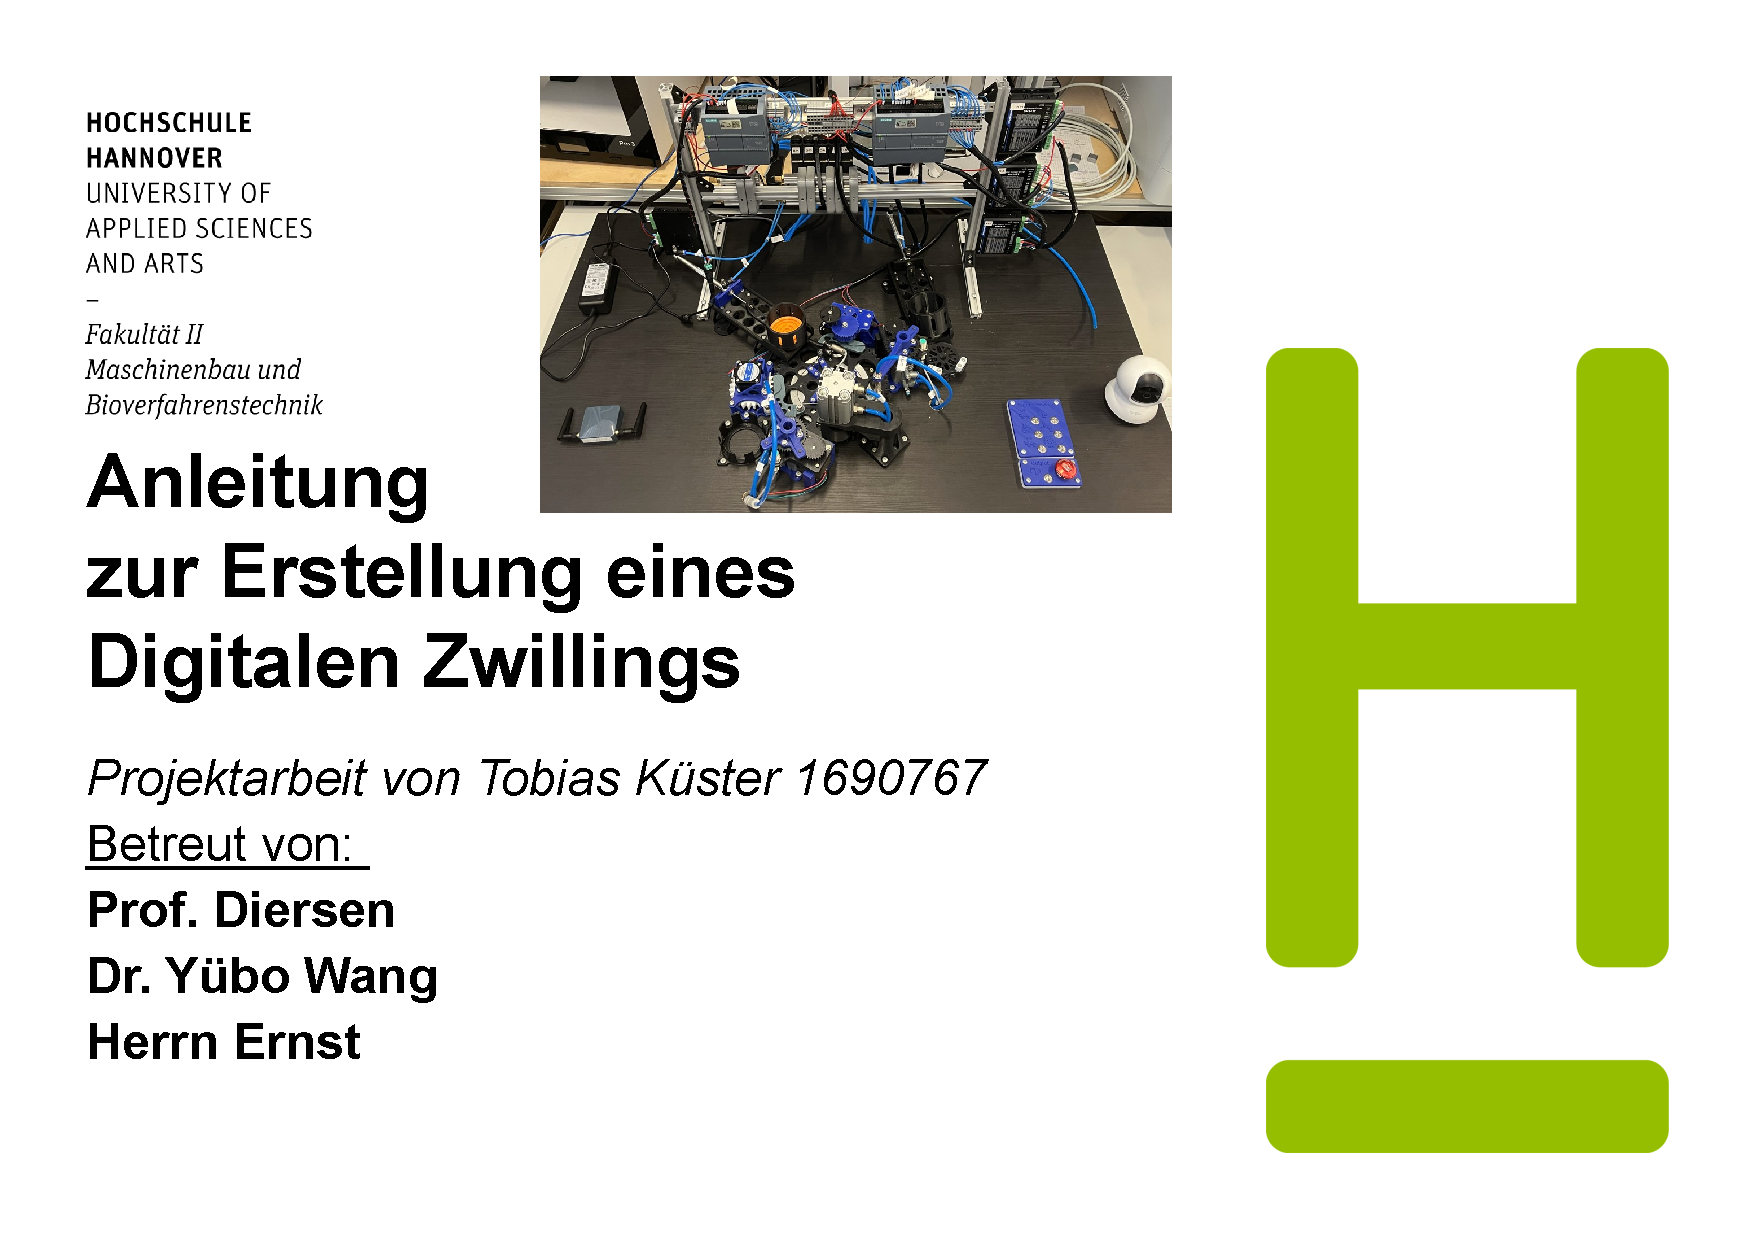
\includepdf[pages=-,pagecommand={\thispagestyle{plain}},fitpaper=true]{Doku_Hinweise_Leitfaeden/Kuester_Omniverse_Tutorial.pdf}

\section{Schnittstellenmatrix Maze Runner (Auszug)}
\label{anhang:schnittstellen}
\begin{table}[htbp]
\centering
\caption{Auszug aus der OPC-UA-Schnittstellenmatrix des Maze Runner}
\begin{tabularx}{\textwidth}{lllX}
\toprule
\textbf{Variable} & \textbf{Datentyp} & \textbf{Richtung} & \textbf{Beschreibung} \\
\midrule
\texttt{TableAngle}     & Float  & R   & Aktueller Drehwinkel des Rundtakttisches in Grad \\
\texttt{TableSpeed}     & Float  & R/W & Soll-/Ist-Drehzahl in U/min \\
\texttt{GripperState}   & Bool   & R/W & Pneumatischer Greifer geöffnet/geschlossen \\
\texttt{SensorStation1} & Bool   & R   & Induktiver Näherungsschalter Station 1 \\
\texttt{EmergencyStop}  & Bool   & R   & Status Not-Halt-Kreis \\
\bottomrule
\end{tabularx}
\end{table}


\end{document}
